\documentclass[12pt,a4paper,oneside,titlepage]{book} %appel de classe
%appel des packages:
\usepackage{fontspec} %package pour gérer les fontes
\usepackage{xunicode} %package pour gérer l'unicode
\usepackage{hyperref}
\hypersetup{
    colorlinks=true,
    linkcolor=blue,
    filecolor=magenta,      
    urlcolor=cyan,
    pdftitle={Overleaf Example},
    pdfpagemode=FullScreen,
    }
\usepackage[french]{babel}
\usepackage[backend=biber, sorting=nyt, style=enc]{biblatex}
\usepackage{csquotes}
\usepackage{graphicx} 
\usepackage{caption}
\usepackage{wrapfig}
\usepackage{parskip}
\usepackage{lettrine}
\usepackage{multirow}
\usepackage{rotating}
\usepackage{subcaption}
\usepackage{booktabs}
\usepackage{amsmath}



\usepackage[margin=2.5cm]{geometry}
\usepackage{setspace}
\setlength{\parindent}{1cm}
\onehalfspacing
\hyphenation{}

\usepackage{tikz}

\usepackage{biblatex}
\addbibresource{bibliographie/Creepypasta.bib}
\usepackage{titlesec}







\setstretch{1,5}
\begin{document}
\frontmatter
%Page de titre
\begin{titlepage}
	\begin{center}
		
		\bigskip
		
		\begin{large}
			UNIVERSITÉ PARIS, SCIENCES \& LETTRES
		\end{large}
		%TODO: nom établissement de préparation
		\begin{center}\rule{2cm}{0.02cm}\end{center}
		
		\bigskip
		\bigskip
		\bigskip
		\begin{Large}
			\textbf{Alexandre Lionnet-Rollin}\\
		\end{Large}
		\begin{normalsize} \textit{licencié ès lettres modernes}\\
			
		\end{normalsize}
		
		\bigskip
		\bigskip
		\bigskip
		
		\begin{Huge}
			\textbf{Quand la peur devient virale}\\
		\end{Huge}
		\bigskip
		\bigskip
		\begin{LARGE}
		\textbf{Exploration d'un genre de littérature numérique virale : les creepypastas}\\
		\end{LARGE}
		
		\bigskip
		\bigskip
		\bigskip
		\begin{large}
		\end{large}
		\vfill
		
		\begin{large}
			Mémoire pour le diplôme de Master\\
			\og Humanités numériques et computationnelles \fg{} \\
			\bigskip
			2025
		\end{large}
		
	\end{center}
\end{titlepage}

\thispagestyle{empty}

\cleardoublepage

\section*{Résumé}
\addcontentsline{toc}{chapter}{Résumé}

Ce mémoire se consacre à l'exploration approfondie des creepypastas, un genre distinct de littérature numérique virale. Pour ce faire, il a mobilisé une approche résolument quantitative, s'appuyant notamment sur les techniques du Traitement Automatique des Langues. Cette méthodologie a permis d'analyser un vaste corpus de textes et de dégager des tendances significatives. L'étude révèle ainsi que, contrairement aux attentes souvent associées à la littérature d'horreur, ces récits se distinguent par une simplicité structurelle notable et une prédominance marquée de thèmes liés à l'intime et à l'expérience personnelle. De plus, l'analyse du lexique a montré une présence étonnamment moins prononcée du vocabulaire horrifique explicite, suggérant que l'effroi dans les creepypastas émane davantage de l'ambiguïté, du familier détourné et de la suggestion, plutôt que de l'horreur graphique ou du grotesque. Concernant la viralité de ces contenus, les résultats de la régression indiquent que les facteurs prépondérants sont la lisibilité du texte et la longueur des phrases, ces éléments ayant un impact plus significatif sur leur propagation que le degré de peur ou les thématiques abordées en elles-mêmes. L’analyse de l’évolution au sein d’une plateforme a permis de confirmer l’hypothèse que certaines plateformes évoluent en fonction d’un historique cumulatif de toute la production depuis leur origine.

\medskip

\textbf{Mots-clés:} Creepypasta, littérature numérique, viralité, TAL, littérarité, internet, horreur, lisiblité, canon littéraire, modélisation

\textbf{Informations bibliographiques:} Alexandre Lionnet-Rollin, \textit{Quand la peur devient virale: exploration d'un genre de littérature numérique, les Creepypastas}, mémoire de Master 2 \og Humanités numériques et computationnelles\fg{}, dir. Florian Cafiero et Jean Baptiste Camps, Université Paris, Sciences \& Lettres, 2025.


\pagebreak
\section*{Abstract}
\addcontentsline{toc}{chapter}{Abstract}

This M.A. thesis is dedicated to the in-depth exploration of creepypastas, a distinct genre of viral digital literature. To achieve this, it mobilized a resolutely quantitative approach, relying notably on Natural Language Processing techniques. This methodology allowed for the analysis of a vast corpus of texts and the identification of significant trends. The study thus reveals that, contrary to expectations often associated with horror literature, these narratives are distinguished by a notable structural simplicity and a marked predominance of themes related to intimacy and personal experience. Furthermore, lexical analysis showed an surprisingly less pronounced presence of explicit horrific vocabulary, suggesting that the dread in creepypastas stems more from ambiguity, familiar elements twisted, and suggestion, rather than graphic or grotesque horror. Regarding the virality of these contents, the regression results indicate that the predominant factors are text readability and sentence length, these elements having a more significant impact on their propagation than the degree of fear or the themes addressed themselves. The analysis of evolution within a platform confirmed the hypothesis that certain platforms evolve based on a cumulative history of all production since their origin.

\medskip

\textbf{Keywords:} Creepypasta, digitial literature, virality, NLP, literariness, internet, horror, readability, modelling, literary canon

\textbf{Bibliographic Information:} Alexandre Lionnet-Rollin, \textit{When fear goes viral: exploring creepypastas, a genre of digital literature}, M.A. thesis \og Digital and computational humanities\fg{}, dir. Florian Cafiero and Jean Baptiste Camps, Université Paris, Sciences \& Lettres, 2025.


\clearpage
\thispagestyle{empty}
\cleardoublepage


\section*{Remerciements}

\lettrine{M}{es remerciements} vont tout d'abord à mes directeurs de recherche. Je tiens à exprimer ma profonde gratitude à M. Florian Cafiero pour sa bonne humeur et son humour et son soutien, tout au long de ces deux années. Ces premiers pas dans le monde universitaire ont été plus facile à faire grâce à vous.

Je tiens à remercier sincèrement M. Jean Baptiste Camps, qui a accepté même tardivement de me diriger et de m'accompagner pour mes débuts dans le monde de la modélisation.

Je souhaite également adresser ma reconnaissance à Mme Valérie Beaudouin pour son accompagnement attentif durant la première partie de ce mémoire.

Ma gratitude va aussi à l’ensemble des enseignants du master Humanités Numériques, et tout particulièrement Chahan Vidal Gorène dont les conseils et l'accompagnement ont grandement contribué à enrichir ces recherches et à rendre ces années plus agréables.

Je remercie chaleureusement Théo Moins et Ulysse Godreau pour leur aide technique précieuse, et pour leur bienveillance malgré mes piètres prestations en live coding…

Je suis aussi très reconnaissant à M. Armin Pournaki pour son aide précieuse dans la recherche et l’exploitation des données, qui a largement contribué à la rigueur de ce travail.

Un immense merci à ma mère pour sa patience infinie et son soutien, même lorsque mes explications embrouillées ont fait d’elle — bien malgré elle — une spécialiste de littérature numérique.

Merci à Eva, ma supportrice indéfectible, qui jusqu'au dernier moment m'a accompagné dans la rédaction et la relecture.

Toute ma gratitude va à mes camarades, avec qui j’ai partagé ces deux années riches et intenses. Leur compagnie, qu’elle fût autour d’un verre ou au détour d’un projet Python, me manquera profondément.

Enfin, je dédie ce travail, en filigrane, à tous les auteurs amateurs, anonymes ou pseudonymes, qui ont nourri mes nuits et allongé mes journées de recherche de leurs créations et toutes les personnes qui de près ou de loin ont rendu tout ça possible.




\clearpage

\thispagestyle{empty}
\cleardoublepage

\tableofcontents


\newpage
\pagenumbering{arabic}

\mainmatter
\chapter*{Introduction}
\addcontentsline{toc}{chapter}{Introduction}
\markright{Introduction}                     % Pour forcer l’en-tête droite (si classe report/book)
\lettrine{I}l arrive qu'une société entière désigne, lors de son apparition, un phénomène comme une menace pour ses valeurs ou ses intérêts, mobilisant médias, institutions et opinion publique dans une réaction collective disproportionnée par rapport à la réalité des faits. Cette dynamique d'amplification sociale, que le sociologue Stanley Cohen a conceptualisée sous le terme de "panique morale"\footcite{cohen2011folk}, révèle moins la dangerosité objective du phénomène en question que les tensions et anxiétés latentes d'une époque.

L'affaire Slender Man, survenue dans le Wisconsin au milieu des années 2010, illustre parfaitement ce mécanisme. Lorsque deux adolescentes tentent d'assassiner leur camarade de classe au nom d'une entité fictionnelle jusque-là confinée aux forums Internet, l'événement déclenche une couverture médiatique nationale qui transforme le Slender Man en symbole d'un Internet dangereux pour les enfants. Né d'un simple photomontage sur le forum \textit{Something Awful}, ce personnage devient instantanément l'incarnation des peurs parentales face aux nouvelles pratiques numériques des adolescents.

Cette réaction révèle un phénomène plus large : l'émergence, depuis le début des années 2000, d'une nouvelle forme narrative numérique que l'affaire a paradoxalement popularisée. Les creepypastas - courtes histoires horrifiques qui circulent de forum en forum - constituent un genre littéraire inédit, mêlant codes de la légende urbaine et spécificités du médium numérique. Ces récits, qui jouent délibérément avec la frontière entre réalité et fiction, illustrent les mutations contemporaines de la création narrative à l'ère du Web participatif.

Pourtant, au-delà du sensationnalisme médiatique, ces productions soulèvent des questions théoriques fondamentales sur les nouvelles modalités de création, de diffusion et de réception littéraires dans l'écosystème numérique contemporain. Comment ces récits, souvent produits anonymement par des amateurs, parviennent-ils à captiver et à se propager massivement ? Quels mécanismes président à leur succès viral ? 


Ce mémoire se propose d'étudier le phénomène des creepypastas comme un laboratoire privilégié pour comprendre les mutations de la culture narrative à l'ère numérique.

\section*{Contexte}

Le début des années 2000 marque l’entrée d’Internet dans la seconde phase de son existence : le Web 2.0, expression popularisée par Tim O'Reilly en 2004, correspond à une période de développement sans pareil de nouveaux canaux de communication. L’avènement des grands réseaux sociaux tout comme les grandes plateformes d’hébergement et de partage de contenus va permettre une nouvelle façon de dialoguer, et de produire du contenu. Cette période marque aussi le développement des ordinateurs personnels et la démocratisation de l'outil numérique pour un usage personnel, et non plus exclusivement professionnel.

Et parmi les nouvelles pratiques permises par ceux-ci, on trouve de nouvelles formes d'écriture, qui renouvellent aussi bien la façon d’écrire que le but des productions. Écriture collaborative, écriture fragmentaire, mais aussi une écriture qui peut, à la manière d'une traînée de poudre, se répandre bien au-delà de leurs sphères de production. Parmi celles-ci, on trouve une écriture simple, et relativement courte, prenant la forme d'un court témoignage, qui rapidement vire au cauchemar : les creepypastas. 
\par
	La première occurrence du terme remonte au mois de juillet 2007 sur le forum \emph{4Chan}\footnote{Le post a depuis longtemps été supprimé. On peut néanmoins en trouver une archive au lien suivant : \url{https://web.archive.org/web/20111207000647/http://chanarchive.org/4chan/b/257/creepypasta}}. Cette dénomination est le fruit de la rencontre entre l'adjectif \emph{creepy} (litt. effrayant) et l'expression \emph{copypasta}, elle-même contraction des verbes \emph{copy} et \emph{paste} (litt. copier, coller), désignant un bloc de texte copié et collé sur différents forums afin de le partager. Si les \emph{copypastas} peuvent traiter de tous les sujets, aussi bien de blagues que d'actualités et autres informations, les creepypastas sont quant à elles cantonnées au domaine du frisson : les creepypastas sont des copypastas dont le but est d'effrayer le lecteur. Ainsi, nous nous appuierons sur les définitions de Joe Ondrak et Trevor Blank pour amorcer notre réflexion :
    
	\begin{quotation}
		[copypastas are] short pieces of prose, sometimes accompanied by an image or a video […] meant to be copied and pasted […] and spread on the Internet via social media, e-mails, and message boards […]whereas copypasta can be about almost any subject, creepypasta is usually aimed at scaring the reader and/or viewer.\footnote{\emph{Les [copypastas sont] de courts morceaux de prose, parfois accompagnés d'une image ou d'une vidéo [...] destinés à être copiés et collés [...] et diffusés sur Internet via les médias sociaux, les courriels et les tableaux d'affichage [...]Alors que le copypasta peut porter sur presque tous les sujets, le creepypasta vise généralement à effrayer le lecteur et/ou le spectateur.}}(Ondrak, 2018 p.162)\footcite{ondrak_spectres_2018}
	\end{quotation}
	\par
	Cette première définition permet de souligner la dualité intrinsèque des CP\footnote{Dans un soucis de clarté, dès à présent et pour le reste de ce mémoire, le mot "creepypasta" sera abrégé en CP.} : d'une part, elles sont définies par leur aptitude à effrayer le lecteur (le caractère horrifique), et d'autre part, par leur capacité à être transmise sur différents canaux. 
    A des caractéristiques s'ajoute une dimension folklorique cruciale, soulignée par Trevor Blank :
\begin{quotation}
    More specifically, it is an emergent genre of Internet folklore that involves the creation and dissemination of a particular style of creative horror stories and images. (Blank, 2018, p.6 )\footcite{blank_slender_2018}
\end{quotation}
Cette inscription dans une logique de diffusion, de transmission et de réappropriation communautaire inscrit d’emblée les CP dans une tradition folklorique renouvelée. C’est précisément sous cet angle qu’elles ont été appréhendées par plusieurs chercheurs : sous la direction de Trevor Blank et Lynne McNeil, deux folkloristes, l'ouvrage \textit{Slenderman is coming}\footcite{blank_slender_2018} explore la notion de croyance populaire à l'ère contemporaine du numérique, en s'appuyant sur principalement sur le cas du slender man évoqué plus tôt. 

Ces cas spécifiques ont été aussi l'occasion pour les chercheurs d'explorer l'aspect communautaire de ces productions, et comment celles-ci permettait la création de communauté et inversement, à l'instar de mythes fondateur d'une culture\footcite{chess2014folklore}.

Si quelques auteurs se sont essayés à proposer une approche plus littéraire de ces productions \footcite{garcia_roca_fundacion_2021}\footcite{garcia_roca_creepypasta_2021}, plutôt que sous l'angle de la communication, du folklore voire de l'anthropologie, les creepypastas restent encore un phénomène plus qu'un genre, souffrant, comme une grande partie des productions littéraires numériques\footcite{lata_du_2022}, d'un manque de légitimité institutionnelle \footcite{saemmer_litterature_2011}, malgré une certaine proximité assumée avec certains genres littéraires connus comme la littérature fantastique par exemple \footcite{evans_slender_2018}, ou encore la massivité du phénomène.

Cette absence de légitimité institutionnelle ne signifie pas pour autant l'absence de processus de canonisation. Comme l'ont montré des études quantitatives récentes sur les textes littéraires (\cite{algee-hewitt-between-2015}, \cite{underwood_distant_2019}), la formation du canon implique généralement un processus à long terme façonné par les institutions académiques, éditoriales et culturelles. Ces institutions, qui médiatisent traditionnellement la reconnaissance des œuvres canoniques, sont absentes dans le cas des creepypastas. À leur place, le « canon » des *creepypastas* émerge de manière organique, porté par les interactions entre utilisateurs, l'adhésion communautaire et les mécanismes de viralité inhérents aux plateformes en ligne.

Mais au-delà de l'aléatoire et des phénomènes de cascade observés dans les mécanismes de « viralité », existe-t-il des déterminants ? Qu'est-ce qui distingue les creepypastas les plus populaires ou « canoniques » des autres ? Bien que le processus de canonisation à long terme observé dans la littérature traditionnelle ne s'applique pas directement, certaines histoires parviennent néanmoins à obtenir une reconnaissance significative et deviennent emblématiques de la culture internet. Comprendre ce qui fait ressortir ces histoires nécessite d'identifier des caractéristiques partagées, qu'elles soient formelles, thématiques ou émotionnelles.

En effet, les creepypastas ne représentent plus un mouvement isolé perdu dans un recoin obscur d'internet. Le \textit{subreddit} /r/nosleep, pôle de référence de production et de consommations, compte près de 190 000 productions, les différents forums dédiés sont riches de dizaines de milliers de productions. Avec la croissance du genre, les productions se sont tournées vers une forme principalement écrite, constituant un corpus textuel d'une ampleur considérable.

Pour autant, malgré cette massivité, seulement une poignée d'exemples ont fait l'objet d'analyses approfondies : le Slender Man, objet du plus grand nombre d'études et d'ouvrages, la fondation SCP\footcite{maurel:dumas-04760430}\footcite{garcia_roca_fundacion_2021}, ou encore Candle Cove \footcite{balanzategui_creepypasta_2019}, sont autant d'exemples canoniques dont il faut questionner la représentativité vis-à-vis des autres productions.

Cette focalisation sur quelques cas emblématiques soulève une question méthodologique fondamentale. La problématique de l'exploration des grands pans de corpus délaissés au profit de productions canoniques n'est pas nouvelle : la notion fondatrice de lecture distante de Franco Moretti \footcite{moretti2013distant} repose précisément sur l'idée d'explorer toute une littérature « abattue » par le canon littéraire traditionnel. De façon analogue, qu'advient-il des histoires qui n'ont pas survécu au processus de sélection des creepypastas ? Quelles caractéristiques distinguent les récits qui perdurent de ceux qui sombrent dans l'anonymat numérique ?

Cette lacune méthodologique s'explique en partie par l'absence d'études quantitatives systématiques sur ce corpus. Les approches qualitatives, bien qu'éclairantes pour comprendre les mécanismes narratifs et culturels à l'œuvre, ne permettent pas de saisir les régularités statistiques qui pourraient révéler les mécanismes sous-jacents de sélection culturelle. L'ampleur du corpus appelle donc des méthodes d'analyse computationnelle capables de traiter massivement ces données textuelles, tout en préservant la finesse d'analyse nécessaire à la compréhension des enjeux littéraires et culturels.

Cette dimension quantitative de l'analyse textuelle s'inscrit assez naturellement dans le champ de l'évolution culturelle. Les travaux pionniers de Boyd et Richerson\footcite{boyd1988culture} ont montré que les phénomènes culturels pouvaient, tout comme les phénomènes biologiques, être analysés au moyen de modèles évolutionnaires. Ces modèles permettent d’étudier la transmission, la mutation ou la sélection des éléments culturels à travers des approches issues des sciences naturelles, comme la biologie par exemple\footcite{el2014cultural}.

Un cas spécifique de cette approche réside dans l'utilisation de tels modèles dans le cadre de la transmission textuelle et de la quantification de perte et de survie d'œuvres. Kestemont et al.\footcite{kestemont2022forgotten} puis Camps et Randon-Furling\footcite{camps2022lostmanuscriptsextincttexts}, faisant suite aux travaux pionniers de Weitzman\footcite{Weitzman1987}, ont ainsi emprunté des outils méthodologiques à l'écologie et à la biologie, utilisant notamment des modèles d'espèces non vues pour estimer la proportion de textes et de manuscrits ayant survécu à travers les siècles. Au-delà des processus stochastiques de naissance et de mort, ces modèles tentent de rendre compte de l'existence de ces éléments textuels qu'on ne peut plus observer directement, ces témoins absents de l'évolution culturelle.
Cette perspective entre en résonance directe avec notre objet d'étude : au-delà des œuvres de creepypastas accessibles et peu connues que nous pouvons analyser, combien sont aujourd'hui perdues dans les méandres d'un blog abandonné ou d'une page personnelle supprimée ? Plus généralement, la modélisation des trajectoires de transmission des creepypastas, qu'il s'agisse de la circulation d'histoires particulières, de l'évolution d'un même trope narratif, ou encore des mécanismes de réplication et de variation de ces récits, s'inscrit naturellement dans cette lignée théorique et mérite d'être expérimentée dans le contexte numérique contemporain.

En parallèle, cette question de la reconnaissance nous amène naturellement à considérer les recherches existantes sur la canonisation littéraire. Les travaux récents en humanités numériques ont en effet démontré qu'il était possible de modéliser en partie la littérarité\footcite{koolen_literary_2020} et d'identifier les éléments textuels qui contribuent à l'évaluation de la qualité littéraire\footcite{van_cranenburgh_identifying_2015}. Dans le contexte français, des recherches ont notamment montré que la canonicité des textes pouvait être partiellement prédite par leurs caractéristiques formelles \footcite{barre_operationalizing_2023}, ouvrant ainsi la voie à une approche computationnelle de la valeur littéraire.

%Parmi les découvertes de ces recherches, les travaux de M. Algee Lewit\footcite{algee2016canon} sur les canons littéraires ont révélé un paradoxe contre-intuitif concernant la richesse lexicale. En analysant le Type-Token Ratio (TTR) – qui mesure la diversité du vocabulaire utilisé dans un texte – ils ont observé que les œuvres canoniques présentaient paradoxalement un TTR plus faible que les textes non canoniques. Autrement dit, les textes reconnus comme littéraires utilisent un vocabulaire moins varié que les autres, suggérant que la répétition et la récurrence lexicale pourraient être des marqueurs de canonicité plutôt que des défauts stylistiques.

%Cette découverte nous a conduits à intégrer le TTR  et d'autres métriques de richesse lexicales dans notre analyse des récits creepypasta, nous demandant si des phénomènes similaires pouvaient être observés dans ce qui constitue un canon natif du numérique. L'hypothèse sous-jacente est que le TTR et d'autres caractéristiques formelles mesurables pourraient servir d'indicateurs pour identifier les facteurs contribuant à l'émergence d'une hiérarchie qualitative au sein de ces productions en ligne.


\section*{Problématisation}

Les creepypastas sont un objet au carrefour des théories, des traditions et des pratiques. Cette étude propose d'explorer ce phénomène et de chercher à le caractériser comme genre avec ses caractéristiques propres. 
Cette recherche poursuit deux objectifs principaux : définir précisément les creepypastas comme genre narratif spécifique, puis identifier et comprendre les mécanismes qui permettent à certaines histoires de se distinguer et d'acquérir un statut de référence. \textbf{Ainsi nous nous demanderons comment l'analyse computationnelle des caractéristiques textuelles (formelles, thématiques et affectives) permet-elle de définir les spécificités des creepypastas en tant que genre de littérature numérique et d'identifier les facteurs contribuant à leur succès viral et à l'émergence d'un canon dans l'écosystème en ligne? }

\section*{Annonce de plan}

Dans un premier temps nous développerons les caractéristiques théoriques des creepypastas comme point de convergence entre traditions narratives et innovations numériques. Il s'agit de montrer comment ces récits articulent des éléments folkloriques anciens avec les nouvelles pratiques et l’imaginaire collectif numérique, produisant une esthétique nouvelle à la croisée des époques et des médias.

Pour appuyer cette analyse théorique, nous présenterons ensuite les données et méthodes qui permettent d'étudier empiriquement ce phénomène. Cette section détaillera la constitution du corpus de plusieurs dizaines de milliers de creepypastas, les outils d'analyse textuelle employés, et les métriques quantitatives utilisées pour mesurer les caractéristiques formelles et thématiques de ces récits.

Puis nous proposerons une caractérisation quantitative du corpus qui dépasse l'approche par cas d'étude pour révéler les régularités statistiques de l'ensemble de la production. En analysant massivement les caractéristiques formelles, syntaxiques, lexicales, thématiques et affectives de ces textes, nous cherchons à identifier les structures invisibles à l'analyse qualitative traditionnelle et àconfirmer les hypiothèses de notre approche théorique.

Enfin dans une dernière partie nous partirons des résultats et des données pour tenter de rendre compte des dynamiques en jeu au sein du corpus, en essayant de caractériser les histoires à succès et de modéliser l'évolution des thèmes au sein d'une plateforme.

\pagebreak
\part{Qu'est-ce-qu'une Creepypasta ?}


\chapter{Une littérature à la frontière des genres}

\section{Folklore à l'ère du numérique, folklore numérique}

Le folklore numérique se constitue à travers des récits, des figures et des rituels propres à l’univers en ligne, produits et perpétués par des communautés d’internautes. Les creepypastas, en tant que récits anonymes ou pseudonymes circulant de manière virale, s’inscrivent pleinement dans cette dynamique. 
Néanmoins, la notion de folklore numérique est loin d'être triviale et a connu de nombreuses redéfinitions et approches \footnote{Pour une chronologie de la notion, voir \cite{de2020digital}}. 

En premier lieu, les creepypastas renouent avec un folklore plus traditionnel dans la forme et dans les thèmes. Par folklore traditionnel, on entend ici l'ensemble des productions culturelles populaires émanant d'un groupe, transmis le plus souvent par voie orale de génération en génération. 
Cette définition apparaît comme limitante du point de vue des CP : que cela soit la notion de génération (impliquant une temporalité bien plus longue) ou bien la voie de transmission orale, les CP ne sont pas des témoins du folklore traditionnel. 
Néanmoins, les CP puisent bel et bien dans ces traditions. Prenons d'abord la forme oralisante du folklore. Malgré une forme écrite, les caractéristiques de la narration,par exemple le récit d'une expérience ou la confession, sont autant d'éléments mimant une transmission orale presque intime à d'autres personnes.
Un des textes canoniques du genre, la première occurrence du phénomène des \textit{Backrooms} joue par exemple sur une forme d'avertissement : 
\par
\begin{quotation}
\textit{Si vous êtes imprudent et que vous \textit{noclipez} de la réalité au mauvais endroit, vous vous retrouverez dans les \textit{Backrooms}, où il n'y a rien d'autre que la puanteur de la vieille moquette humide, la folie du monochrome jaune, au bourdonnement incessant des néons, piégé dans approximativement 600 millions de miles carrés de pièces vides segmentées au hasard. Que Dieu vous protège si vous entendez quelque chose errer à proximité, parce qu’il est certain que cette chose vous a entendu.}
\end{quotation} \label{txt:backrooms}

On retrouve dans ce texte l' \og imprudence\fg{}, le mauvais endroit, l'idée d'un piège dans lequel on tomberait, et enfin le danger émanant de cet endroit, conséquence de l'imprudence. 
Difficile de ne pas penser en lisant ce texte aux contes d'avertissement, certes parodiés ici, mais dont la vocation première est la sensibilisation, sous forme d'image, au danger que représente le monde. \footnote{Nous retraiterons plus en détail de cette histoire dans une partie suivante (voir \ref{backrooms} }

Mais au-delà de la réappropriation, les CP peuvent être considérées comme des éléments du folklore numérique, c'est-à-dire l'ensemble des pratiques, contenus et formes de communication créés et partagés par les utilisateurs sur Internet. Il s’agit d’une culture populaire née en ligne, qui, bien que souvent perçue comme anodine, joue un rôle central dans notre usage quotidien des médias numériques.
%transition
Cette conceptualisation des Creepypastas s'inscrit dans le cadre théorique du folklore numérique, développé depuis les années 1990 pour analyser les nouvelles formes culturelles nées sur Internet. Ce concept englobe les pratiques créatives des utilisateurs en ligne : mèmes, blagues, récits partagés, qui constituent une culture populaire spécifiquement numérique.

Les Creepypastas illustrent parfaitement cette dynamique. Elles représentent une \textbf{créativité vernaculaire} - c'est-à-dire une production culturelle amateur qui émerge "d'en bas", créée par les utilisateurs pour les utilisateurs, en dehors des circuits institutionnels traditionnels. Cette dimension amateur ne signifie pas manque de qualité, mais appropriation créative des outils numériques par des communautés d'utilisateurs.

Ces récits combinent traditions narratives anciennes (contes d'avertissement, légendes urbaines) et spécificités du médium numérique. Contrairement aux formes traditionnelles, les Creepypastas populaires font l'objet de \textbf{réécritures constantes} : traductions, adaptations, variations qui créent une multiplicité de versions. Cette variabilité constitue une caractéristique structurelle du folklore numérique, rendue possible par la facilité de copie et de modification des contenus en ligne.

La circulation de ces récits contribue également à la \textbf{formation de communautés} partageant codes et références communes. Leur discussion collective participe de la "socialité numérique", créant des liens sociaux médiatisés par les technologies, comme en témoigne la naissance de plateforme dédiée à ce genre.

Les Creepypastas soulèvent enfin des questions d'\textbf{authenticité} particulièrement révélatrices de la culture numérique. Beaucoup jouent sur l'ambiguïté fiction/réalité ("Est-ce vraiment arrivé ?"), tandis que l'anonymat fréquent des auteurs facilite l'appropriation collective. Ces caractéristiques illustrent les transformations de l'autorité culturelle à l'ère numérique.

Penser les CP comme une forme de folklore, c'est donc penser ces histoires comme bases d'une culture commune à un groupe, restreint dans la plupart des cas, mais pouvant s'élargir au gré de la dispersion sur la toile. 

\begin{wrapfigure}{l}{0.38\textwidth}
\centering
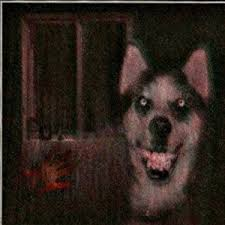
\includegraphics[width=0.35\textwidth]{illustration/smile_dog.jpg}
\small
\caption{L'image hantée de l'histoire \textit{Smile Dog} : cette image apparaît à la toute fin de la creepypasta.}
\label{fig:smile_dog}
\end{wrapfigure}

Or en plus de la base textuelle de ces histoires, les illustrations et l'utilisation de média visuel jouent un rôle important que nous serons amenés à développer. Nous évoquions l'idée d'un imaginaire collectif, alimenté par les creepypastas : l'image est un vecteur plus puissant encore de symbole et d'élément identifiable à même d'être reconnu ou réemployé dans d'autres contextes. En effet, il est plus facile de dégainer une image horrifiante que de prendre le temps de raconter l'histoire qui lui est associée.

L'histoire du \textit{Smile Dog}\footnote{\url{https://creepypasta.fandom.com/wiki/Smile_Dog}} par exemple, est une histoire textuelle. Pour autant c'est l'image clé (cf. \ref{fig:smile_dog}) de cette histoire dont les personnes se souviennent. L'histoire est racontée par un jeune chercheur qui investigue sur une légende urbaine, celle d'une image qui hanterait toute personne qui la voit jusqu'à ce que celle-ci soit montrée à quelqu'un d'autre, sans qu'on puisse en trouver trace. L'histoire se conclut sur le narrateur transmettant à son tour l'image.
La pierre angulaire de l'histoire est à la fois l'image comme média et comme thème : en jouant sur la frontière fiction/réel à travers une approche métatextuelle, l'histoire illustre la puissance à la fois de l'image et la question de l'authenticité mentionnée plus tôt.

Le cas d'utilisation d'une image dans le cadre des CP est loin d'être un épiphénomène: nous allons voir que la multimodalité est un des éléments caractérsitiques du genre.
\section{Une littérature multimodale}

Le numérique fait partie intégrante de l’identité des CP. Rappelons ainsi notre définition de départ : les CP sont avant tout des productions littéraires sur Internet destinées à la diffusion sur Internet. 

	\begin{wrapfigure}{r}{5cm}
	\centering
	
\includegraphics[scale=0.35]{illustration/ben_drowned1}
	\caption{\small Un statue invoqué par le joueur: elle ne bouge pas et le suit durant sa partie, générant un malaise nouveau, absent de l'expérience de jeu originale.}
	\label{img:ben_drowned}
\end{wrapfigure}

Ces objets nativement numériques ne le sont pas seulement par leur existence sur Internet mais aussi par la forme qu’ils prennent : il est fréquent que les CP soient des productions multimodales, faisant intervenir d’autres médias, comme la vidéo, la photographie ou la musique. Notons par exemple la CP \emph{Ben Drowned}\footnote{\url{https://creepypasta.fandom.com/wiki/BEN_Drowned}}: classique du genre, cette CP raconte l’histoire d’un jeune homme jouant au jeu vidéo \emph{The Legend of Zelda : Majora's Mask} acheté dans une mystérieuse brocante. \\
Le récit du narrateur, constitué d'expérience de jeu et de son ressenti, est entrecoupé d'extraits vidéo issus du jeu, montrant les différents \textit{bugs} ou distorsions absents du jeu original (cf. Figure \ref{img:ben_drowned}).

En plus de la forme que prend l'histoire, la notion de numérique se trouve aussi au coeur de la narration en tant que thème. Au-delà de la mention de l'outil numérique, la technologie joue souvent un rôle cadrant dans le récit, créant ainsi un effet de proximité intéressant : le lecteur lit une histoire sur Internet, grâce à un ordinateur, qui traite d'ordinateur ou affiliés.



\section{Le genre de l'\emph{analog horror}}

Puisant dans le genre du \textit{Found footage} \footnote{enregistrement trouvé}, un genre cinématographique où l'enregistrement est supposément une bande redécouverte, dans lequel on apprend le sort, souvent funeste, des précédents propriétaires,  l'horreur analogique utilise ou émule le format analogique des anciens médias pour raconter une histoire dérangeante, souvent sur le plan psychologique (en opposition avec une horreur spectaculaire par exemple) 
L'aspect dérangeant vient dans un premier temps du contraste entre l'aspect réconfortant du numérique et sa déformation plus ou moins appuyée \footcite{balanzategui_creepypasta_2019}.

La vidéo, quand vidéo il y a, réplique souvent le format VHS. Ce format est une norme d'enregistrement vidéo sur bande magnétique, en l'occurrence la cassette. Si la majorité des consommateurs aujourd'hui n'ont pas connu directement l'âge d'or des VHS, celle-ci est facilement associée aux productions remontant à l'époque de leurs parents, et donc potentiellement aux premières expériences de visualisation de contenu vidéo durant l'enfance, faisant ainsi du format VHS un vecteur de nostalgie.

Si les exemples sont nombreux dans le domaine du cinéma (on peut ici penser aux films \emph{The Blair Witch Project}\footcite{myrick_blair_1999}, ou bien encore \emph{Paranormal Activity} plus récemment), on en retrouve plusieurs occurrences parmi les CP les plus iconiques : les séries de vidéos inspirées par des CP comme la série \emph{Marble Hornets}\footcite{marble_hornets_introduction_2009} ou \emph{The Backrooms}\footcite{kane_pixels_backrooms_2022} en sont les parfaites représentantes.

Reprenons notre cas précédent : BEN drowned se construit sur un jeu relativement ancien, \textit{Zelda Majora's Mask}, qui pour beaucoup a constitué une si ce n'est la première expérience du jeu vidéo. Ainsi le rapport au jeu est nimbé d'une aura de nostalgie presque indépassable. Dès lors l'horreur de cette histoire joue sur la nostalgie de l'expérience et la différence qu'il existe entre le souvenir et la version déformée proposée. 

\section{La littérature fantastique}
\label{litt-fant}

Sous les différentes publications, il n'est pas rare de trouver des commentaires de ce style :\og Est-ce que c'est réel ?\fg{}.

Si certains répondent souvent avec un peu de mépris à l'internaute qui a le malheure de poser cette question, celle-ci reste fondamentale. Ces histoires sont caractérisées par le fait que le temps de la lecture, elle brouille momentanéement notre percpetion de ce qui est réel ou non.

Tzvetan Todorov, dans son \emph{Introduction à la littérature fantastique}\footcite{todorov_introduction_1992} propose comme première définition du genre fantastique cette dichotomie: 

	\begin{quotation}
Le fantastique, c’est l’hésitation éprouvée par un être qui ne connaît que les lois naturelles, face à un évènement en apparence surnaturel. (Todorov, 1970, p. 27)\newline
	\end{quotation}

Cette "hésitation" se trouve aussi bien du côté du personnage que du lecteur : 
\begin{quotation}
	Le fantastique implique donc [...] l’existence d’un évènement étrange, qui provoque une hésitation chez le lecteur et le héros [...](Todorov, 1970)
\end{quotation}

Cette définition de la littérature fantastique se trouve êtr pertinent pour qualifier l'expérience dans notre cas. À l'instar des nouvelles fantastiques, les creepypastas sont écrites à la première personne. Ce style d'écriture va créer durant la lecture une sorte d'identité entre le lecteur et le narrateur. Cette identité va être renforcé par le cadre familier souvent développé. Ainsi quand le narrateur doute, nous, lecteur, ne ne pouvons nous empêcher de douter aussi. 
\par
En plus de la façon de raconter, les thèmes en eux-mêmes sont proches de ceux employés par ce genre littéraire, à quelques exceptions près. Les monstres traditionnels, s’ils sont souvent présents, laissent place dans de nombreux cas à des éléments tout aussi effrayants, mais beaucoup plus pernicieux : des éléments de notre quotidien, et particulièrement l’outil numérique, plaçant les histoires en adéquation avec des thèmes de sa génération \footcite{king_anatomie_2020}.
\par
Notons par exemple la CP \emph{Candle Cove}\footnote{\url{https://ichorfalls.chainsawsuit.com/}} qui prend la forme d’une discussion sur un forum entre plusieurs utilisateurs se remémorant une émission dérangeante de leur jeunesse. Les souvenirs des uns et des autres s’ajoutent, aussi bien que les détails perturbants, jusqu’à ce qu’un utilisateur souligne le fait que sa mère s’inquiétait de le voir regarder la neige de la télévision lorsque celui-ci prétendait y voir ladite émission. 

\par

Alors que le numérique prend une place grandissante dans la vie quotidienne, allant au-delà du hobby ou de la passion, la perversion de celui-ci, sous toutes ses formes (télévision, film, ordinateur ou bien très souvent Internet) est d'autant plus efficace d'un point de vue de l'horreur: jouer sur la fine frontière entre le réel et la fiction lors de l'expérience de lecture permet de révéler un potentiel horrifique alors inconnu à tous les pbjets qui nous entoure. 
\par
%Transition
Ces éléments témoignent d'un ancrage résolument contemporain des creepypastas, qui ne se contentent pas d'imiter les codes narratifs des genres littéraires traditionnels, mais les réactualisent à travers les objets, les angoisses et les usages propres à l'ère numérique. Ce n'est pas seulement le retour des figures monstrueuses qui fait frissonner, mais bien la manière dont elles s'infiltrent dans les interstices du quotidien contemporain, en particulier dans notre rapport intime aux technologies.
Les creepypastas opèrent ainsi comme un carrefour singulier entre deux univers distincts : d'une part, ils puisent dans le répertoire du folklore et de la tradition littéraire fantastique ; d'autre part, ils s'ancrent profondément dans la culture numérique, tant par leurs thèmes que par leur forme narrative qui assume pleinement cette modernité technologique. En s'érigeant comme récits recombinants \footcite{jacobs_character_1990} qui mêlent systématiquement le neuf au vieux, l'innovation au patrimoine, cette convergence narrative peut être analysée à la lumière du concept de culture de la convergence développé par Henry Jenkins \footcite{jenkins_convergence_2006}.
\section{Les Creepypastas comme lieu de convergence ? }

Henry Jenkins a principalement exploré la convergence entre une culture industrielle traditionnelle, dominée par de grandes compagnies et sociétés de productions, et une culture numérique émergente, caractérisée par la collaboration et la participation active des individus. Pour Jenkins, la culture de la convergence repose sur trois piliers interdépendants : la convergence technologique (fusion des supports médiatiques), la convergence économique (concentration des industries culturelles) et la convergence culturelle (participation active des audiences). Cette dernière dimension transforme les consommateurs en "prosumers", acteurs hybrides qui consomment et produisent simultanément du contenu. Cependant, ce modèle présuppose une hiérarchie entre producteurs institutionnels et audiences participatives, dynamique qui se révèle inadéquate pour appréhender l'écosystème des creepypastas.

Dans le contexte des creepypastas, cette hiérarchie traditionnelle n'est pas aussi pertinente. En effet, les creepypastas sont des œuvres nativement numériques, où le rôle des médias traditionnels n'est pas aussi central. Ces productions émergent directement des communautés en ligne, sans médiation institutionnelle préalable, et évoluent selon des logiques collaboratives qui échappent aux schémas industriels classiques. Ainsi, la dynamique de convergence se manifeste davantage à travers une analogie entre les médias et canaux traditionnels d'une part, et les grandes creepypastas qui agissent comme un canon de la culture numérique, d'autre part.

Cette dynamique canonique s'illustre parfaitement avec la Fondation SCP , qui a établi un univers narratif cohérent régi par des règles strictes de rédaction et de classification, mimant les structures institutionnelles tout en restant entièrement collaborative. De même, \textit{Slender Man}, née sur le forum \textit{Something Awful }en 2009, s'est rapidement imposée comme une figure archétypale générant ses propres codes iconographiques et narratifs, reproduits et déclinés à travers d'innombrables variations. Ces œuvres fonctionnent comme des matrices génératrices, établissant des conventions esthétiques et narratives que la communauté s'approprie et réinterprète. Elles créent leurs propres traditions, leurs propres références canoniques, à la manière des grands cycles mythologiques ou des genres littéraires établis.

Il est essentiel de souligner la distinction du cadre théorique entre la culture de la convergence traditionnellement étudiée par Jenkins et la convergence observée dans le contexte des creepypastas. Alors que Jenkins se concentre sur la fusion entre les industries médiatiques traditionnelles et les nouvelles formes de médias numériques, l'analyse des creepypastas révèle une convergence plus subtile entre les traditions narratives anciennes et les formes d'expression contemporaines, façonnées par l'ère numérique. Cette convergence spécifique se manifeste concrètement dans la façon dont les creepypastas puisent dans l'imaginaire folklorique – l'enfant fantôme, la forêt menaçante, l'expérimentation interdite – tout en exploitant les possiblités offertes par la plateforme numérique: l'anonymat des forums, la viralité des réseaux sociaux, l'interactivité des hyperliens.

Cette capacité des creepypastas à générer leurs propres canons tout en se nourrissant de traditions narratives préexistantes révèle un mécanisme de reproduction culturelle particulier. Les œuvres les plus marquantes ne se contentent pas de converger vers un public, elles deviennent des modèles réplicables, des matrices narratives qui appellent la variation et la réappropriation. Cette logique de reproduction-variation, où chaque itération conserve des éléments structurants tout en introduisant des mutations, évoque les mécanismes décrits par Richard Dawkins dans sa théorie du mème culturel. Ainsi, la convergence dans le domaine des creepypastas offre un exemple unique et éclairant de l'évolution des cultures narratives à l'ère numérique, préparant le terrain pour une analyse de ces productions sous l'angle de la théorie mémétique.


\chapter[Les CP: du pareil au mème ? ]{Les CP, du pareil au mème ? Un mème aux trajectoires multiples}



Cette capacité des creepypastas à générer leurs propres canons tout en appelant constamment la variation et la réappropriation nous conduit naturellement vers une autre dimension fondamentale de ces productions : leur trajectoire de diffusion. En effet, cette notion de parcours, de circulation à travers les espaces numériques, nous permet de revenir au second élément de définition d'une creepypasta. Nous avons mentionné jusqu'ici l'importance de la forme, du caractère terrifiant, percutant et facilement réplicable. Ce dernier aspect – la réplicabilité – révèle en réalité la nature profonde des creepypastas comme productions culturelles conçues pour être partagées, copiées, et transformées dans l'acte même de leur transmission. 

Cette caractéristique fondamentale – celle d'un élément culturel dont l'existence même dépend de sa capacité à être reproduit et propagé – correspond précisément à la définition du mème telle qu'établie par Richard Dawkins dans les années 1970 \footcite{dawkins_selfish_1989}. Dès lors, analyser les creepypastas à travers le prisme de la théorie mémétique permet d'éclairer non seulement leurs mécanismes de diffusion, mais aussi leur évolution et leur persistance dans l'écosystème culturel numérique.


    \section{Les creepypastas comme mèmes}

R. Dawkins définit le mème en étendant la conception du gène à un élément culturel : le mème, à l'instar du gène, constitue un réplicateur qui se transmet non pas par reproduction biologique, mais par imitation entre membres d'un même groupe. Cette approche théorique, formulée dans les années 1970, a connu une transformation conceptuelle majeure avec l'avènement d'Internet.

\subsection{Une théorie évolutive adaptée au numérique}

La notion de mème a évolué de manière significative dans l'environnement numérique. Limor Shifman observe que les mèmes numériques ne circulent plus seulement par \og contagion mentale \fg{}, mais deviennent des \og collections de textes facilement consultables par les utilisateurs \fg{}, libérés de leur cadre biologique initial pour constituer une véritable catégorie analytique \footcite{shifman_cultural_2014}[p.~18]. L'appropriation du terme \og mème \fg{} par les internautes pour désigner les \og idées ou phénomènes largement propagés \fg{} \footcite{knobel_online_2007}[p.~199] a paradoxalement assuré sa survie dans le lexique des études numériques, témoignant d'une intuition collective sur l'existence de mécanismes spécifiques de reproduction culturelle en ligne.

Cette évolution conceptuelle s'avère particulièrement éclairante pour analyser les creepypastas. Ces récits d'horreur numériques ne se contentent plus de circuler par simple imitation : ils forment des ensembles textuels structurés, archivés et manipulables par les communautés d'utilisateurs. Leur raison d'être réside précisément dans leur capacité à être imitées et répliquées --- une vocation que révèle déjà l'étymologie du terme \og copier-coller \fg{}.

Cette perspective actualisée nous amène à poser la question fondamentale : comment une creepypasta survit-elle dans le \og pool \fg{} (\textit{sic}) de récits d'horreur numériques ? Plutôt que d'appliquer mécaniquement le modèle biologique de Dawkins, nous proposons de reconnaître comment l'environnement numérique transforme les modalités de reproduction culturelle. Les trois caractéristiques essentielles identifiées par Dawkins --- longévité, fidélité de copie et fécondité --- deviennent ainsi des outils d'analyse heuristiques pour comprendre la dynamique des creepypastas.

\subsection{La longévité dans l'écosystème numérique}


La longévité d'un mème correspond à la durée de vie d'une copie particulière dans le temps. Dans le contexte numérique, cette notion acquiert une dimension nouvelle et paradoxale. D'un côté, Internet offre théoriquement une persistance temporelle accrue grâce au support numérique. De l'autre, le web ne constitue pas une archive infinie : de nombreux contenus disparaissent, comme l'\emph{ARG} \href{https://www.youtube.com/watch?v=x-pj8OtyO2I}{\emph{This House has people in it}}, dont la majorité des ressources demeure aujourd'hui inaccessible. Une partie des expérimentations hypertextuelles ou multimodale s'est longtemps appuyée sur la technologie Flash par exemple. Avec la fin de cette technologie, les productions ont disparu, faute d'archivage adéquate

Cette fragilité de l'archivage numérique soulève des questions méthodologiques cruciales. Retrouver les traces d'évolution des creepypastas à travers les archives du web --- qu'elles soient institutionnelles ou participatives --- demeure une entreprise complexe, nécessitant des outils spécialisés. Malgré ces disparitions, les histoires les plus virales laissent des traces exploitables dans l'écosystème numérique.

Il est particulièrement remarquable que cette notion de longévité s'intègre dans la thématique même des creepypastas, notamment à travers le concept de \textit{lost media}. Des récits comme \textit{Squidward Suicide}\footnote{\url{https://creepypasta.fandom.com/wiki/Squidward\%27s\_Suicide}}, qui décrit la découverte d'un épisode troublant de \textit{Bob l'éponge} par un stagiaire de Nickelodeon, exploitent précisément cette fragilité mémorielle des médias. Ces histoires transforment la non-longévité en ressort narratif, où la disparition d'un contenu original ne laisse subsister qu'un témoignage, seule trace d'une existence hypothétique.

\subsection{La fidélité de copie : préserver l'essence narrative}
\label{meme_fidelité}
Dans l'environnement numérique, la fidélité de copie ne réside pas dans l'exactitude littérale de la reproduction --- chaque itération pouvant connaître des suppressions ou des ajouts progressifs --- mais dans la capacité à préserver et transmettre le cœur narratif de l'histoire. Cette \og base essentielle \fg{} constitue l'ADN culturel du récit, sa structure profonde qui garantit sa reconnaissance et sa compréhension.

Le trope de l'épisode perdu illustre parfaitement ce mécanisme adaptatif. Les creepypastas exploitant ce motif narratif ne se contentent pas de le reproduire : elles l'actualisent et le réinventent, devenant ainsi des vecteurs de reproduction du mème \og épisode perdu \fg{}. Cette dynamique révèle comment la fidélité s'exprime non par la répétition à l'identique, mais par la transmission créative d'une structure narrative reconnaissable.

Cette approche soulève une question théorique cruciale : comment délimiter la frontière entre le mème du \og média perdu \fg{} en tant que structure narrative abstraite et l'histoire concrète qui l'incarne ? La réponse réside dans la compréhension que la fidélité numérique opère à un niveau structurel plutôt que littéral.

\subsection{La fécondité : mesurer l'impact créatif}

La fécondité constitue la caractéristique la plus révélatrice de la dynamique mémétique numérique. Elle mesure la capacité du mème à générer des répliques de lui-même, et présente l'avantage d'être plus facilement quantifiable. Dans le contexte des creepypastas, cette fécondité se manifeste selon deux modalités complémentaires.
\begin{itemize}
    \item La reproduction directe correspond au nombre de copies \textit{stricto sensu} de chaque histoire. Cette mesure quantitative englobe les republications exactes ou quasi-exactes d'une creepypasta sur différentes plateformes. Cette circulation horizontale témoigne de l'attractivité immédiate du contenu et de sa capacité à susciter le partage dans ses premiers moments d'existence.
    \item La reproduction générative concerne le nombre de \og descendants \fg{} ou variations engendrés par une creepypasta originelle. Ce phénomène se manifeste par la création de nouvelles histoires inspirées, de suites non officielles, de réinterprétations dans d'autres médias, ou d'adaptations transmédiatiques.
    
\end{itemize}

Cette fécondité générative révèle la dimension participative de la culture numérique. Elle transforme les consommateurs de contenu en producteurs potentiels, créant un écosystème culturel auto-entretenu où chaque réception peut devenir une nouvelle création. Cette dynamique s'inscrit dans la logique des communautés en ligne, où la frontière entre auteur et lecteur s'estompe au profit d'une créativité collaborative.

\subsection{Vers une mémétique numérique ? }

L'analyse de ces trois caractéristiques adaptées révèle comment les creepypastas fonctionnent comme des mèmes spécifiquement numériques. Leur longévité dépend des infrastructures d'archivage du web et de leur capacité à transformer la fragilité mémorielle en ressort narratif. Leur fidélité se mesure à la préservation de structures narratives essentielles plutôt qu'à la reproduction littérale. Leur fécondité se manifeste dans la capacité à générer des variations créatives au sein des communautés d'utilisateurs.

Cette approche actualisée de la théorie mémétique offre une perspective analytique  adaptée aux phénomènes culturels numériques. Elle permet de comprendre comment les récits d'horreur contemporains s'inscrivent dans une économie de l'attention et de la participation qui redéfinit les modes traditionnels de circulation narrative. Comme le souligne Sean Rintel, malgré les critiques de réductionnisme, cette métaphore demeure un outil analytique pertinent pour comprendre la diffusion des contenus numériques \footcite[p.~255]{rintel_crisis_2013}, à condition de l'utiliser comme un cadre heuristique plutôt que comme une loi biologique rigide.


\section{Les différentes trajectoires d'une creepypastas}
Toutefois, cette grille théorique ne saurait épuiser la diversité des parcours qu'empruntent concrètement les creepypastas dans l'écosystème numérique. Au-delà des mécanismes généraux, l'observation des pratiques révèle une typologie de trajectoires distinctes, chacune obéissant à ses propres logiques de propagation et d'appropriation communautaire.
	\subsection{Les super CP}
    Il arrive que certaines histoires, fortes de leur succès, deviennent incontournables. Au-delà du genre des CP, ces histoires sont devenues des points de référence d'un imaginaire collectif horrifique en ligne, renouant 

    \subsubsection{SCP-173}
	
	Parmi les grandes CP qui ont traversé le paysage internet, SCP-173\footnote{\url{http://fondationscp.wikidot.com/scp-173}} passe difficilement inaperçue. Apparue sur le sous-forum /x/ de \emph{4Chan}, cette CP est composée d'un court texte et d'une image (voir Figure \ref{img:scp_173}). À l'image dérangeante d'une statue anthropomorphe s'ajoute un court teste où l'entité photographiée est décrite, de telle sorte à nous laisser penser qu'un organisme para-gouvernemental s'en occupe, mais surtout de telle sorte à ce qu’on comprenne que cette créature n'est pas la seule retenue dans l’ombre.  Le texte laisse volontairement des zones de flou : certaines informations sont caviardées, le nom de l'objet (SCP-173) laisse entendre la présence de 172 autres entités, le sigle \og SCP\fg{} n'est pas développé etc... À l'instar d'un lancement \textit{in medias res} le lecteur est projeté pendant un court instant dans un univers sémantique familier mais déroutant, où tout est considéré comme acquis, mais rien n'est expliqué.

		\begin{wrapfigure}{l}{0.5\textwidth}
		\centering
		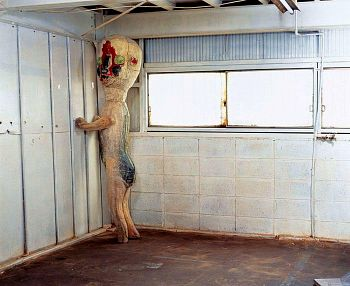
\includegraphics[scale=0.5]{illustration/SCP_173.jpg}
		
		\caption{\small \emph{Untitled 2004} créée par Izumi Kato. Cette photographie a été prise par Keisuke Yamamoto.}
		\label{img:scp_173}
	\end{wrapfigure}
	
	Durant plusieurs jours, SCP-173 s'est retrouvé copié puis collé (complétant ainsi, avec le caractère terrifiant son appellation de CP) sur le sous-forum /x/ puis sur la page d'accueil du site (le \textit{board} /b/), jusqu'à ce que d'autres utilisateurs se joignent au mouvement et produisent à leur tour d'autres CP inspirées par la forme et l'univers de cette CP originelle.
	C'est la suite de son cheminement qui fait passer cette histoire de simple CP à véritable canon : au fil des mois puis des ans, la communauté qui s'est construite autour de SCP-173 et de ce qu'on nomme désormais la \emph{Fondation SCP} s'est autonomisée, créant un wiki , c'est à dire un site collaboratif où chacun peut modifier ajouter et supprmier du contenu, (une première fois grâce au CMS \emph{EditThis} puis au CMS \emph{Wikidot}) puis continuant de croître. Aujourd’hui la \emph{Fondation SCP} est présente dans 12 langues différentes et est forte de plusieurs milliers de productions originales dans chacune de celles-ci \footnote{L'histoire de la Fondation SCP et du parcours de cette histoire originelle est retracée sur \href{http://fondationscp.wikidot.com/history-of-the-universe-part-one}{ces pages}du site.}.

\subsubsection{Slender Man}

Courant 2009, lors d'un concours de photo montage sur le forum \textit{Something Awful}, forum référence dans la production et la consommation de contenu d'horreur en ligne, Victor Surge, un des utilisateurs du forum, publie deux photos. Sur ces deux photos, derrière des groupes d'enfants, on peut apercevoir une silhouette longiligne, au visage d'un blanc laiteux. Ces deux photos sont accompagnées de courts rapports, au ton officiel concernant la silhouette, surnommée \textit{the Slender Man} \footnote{litt. L'homme élancé, en référence à son allure}. 

%année ? 

\begin{figure}[htbp]
    \centering
    \begin{subfigure}[b]{0.45\textwidth}
        \centering
        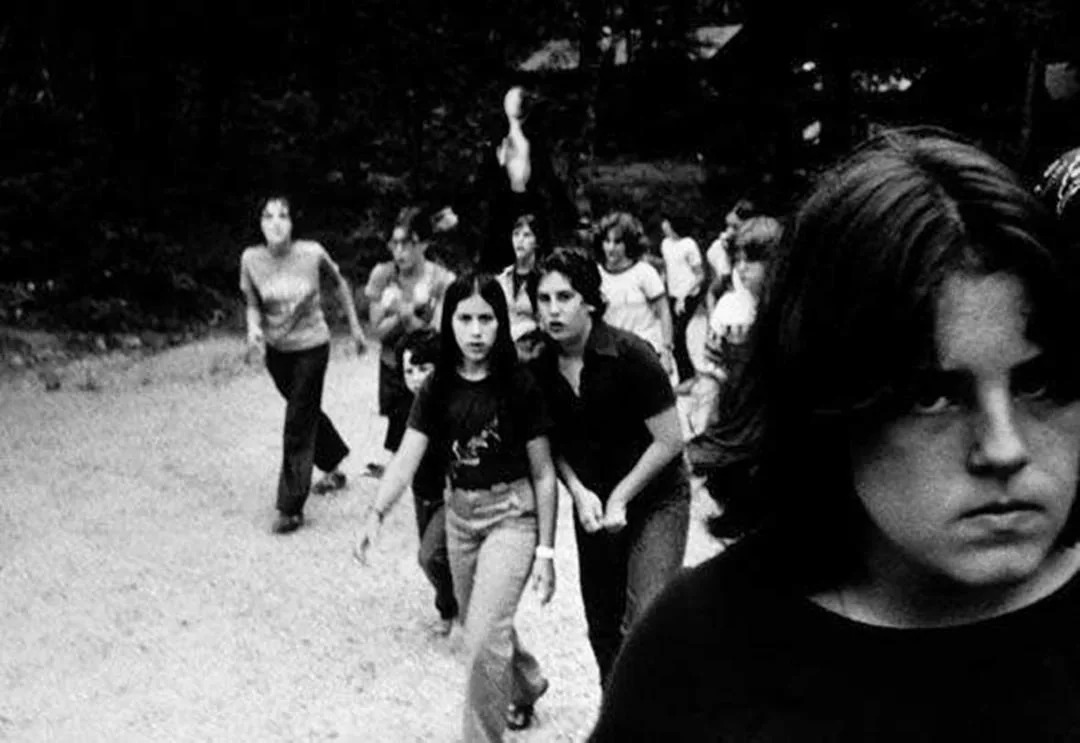
\includegraphics[width=\textwidth]{illustration/photos_slender.jpg}

        \label{fig:slender1}
    \end{subfigure}
    \hfill
    \begin{subfigure}[b]{0.45\textwidth}
        \centering
        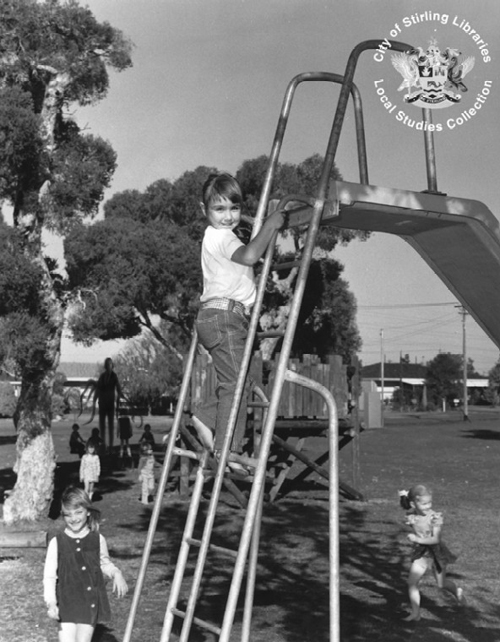
\includegraphics[width=\textwidth]{illustration/slender2.jpg}
        \label{fig:slender2}
    \end{subfigure}
    \caption{Photos montages}
    \label{fig:slender_composite}
\end{figure}

Montages après montages, les quelques lignes les accompagnant nourrissent l'imagination et la créativité des autres utilisateurs : c'est la naissance de la première mythologie Slender Man. 
Le point critique dans la trajectoire de l'histoire est rapidement atteint \footnote{10 jours après la publication originelle} lorsque Troy Wagner publie la première vidéo de la série \textit{Marble Hornets}, comptabilisant aujourd'hui plusieurs dizaines de millions de vues. Ces vidéos mettent en scène le personnage de Jay qui découvre les enregistrements mystérieusement abandonnés de son ami. On apprend rapidement que cet ami était poursuivi par l'\textit{Opérateur}, nom donné dans l'histoire au Slender Man. 

L'explosion en popularité va dans un premier temps développer un véritable univers étendu, où différentes mythologies et origines se superposent concernant le Slender Man. Pouvoirs supplémentaires, objectifs, apparences : autant de caractéristiques qui ont fluctuer avec l'extension du canon. 

Finalement l'incursion de cette histoire dans la réalité, va permettre au Slender Man de se hisser dans la culture populaire, finissant la trajectoire de cette histoire en dehors même de son univers de création.

 \subsubsection{The Backrooms}
\label{backrooms}


\begin{wrapfigure}{r}{0.4\textwidth}
    \begin{center}
        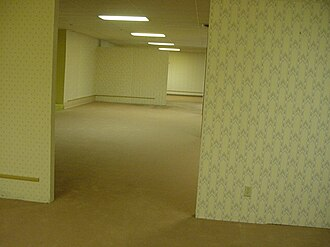
\includegraphics[width=0.38\textwidth]{illustration/backrooms.jpg}
        \caption{L'image originale des Backrooms : l'origine même de l'image fait encore aujourd'hui l'objet d'une quête des internautes}
    \end{center}
    
\end{wrapfigure}

C'est bien plus tard, chronologiquement parlant, que la dernière histoire apparaît. Alors que quelques années à peine séparent l'apparition de SCP-173 et de Slender Man, c'est en 2020 sur le forum 4Chan qu'est publiée anonymement cette fois-ci, une image de bureau vide, au papier peint jaunâtre, accompagnée d'un court texte (cf. \ref{txt:backrooms}). La description de cet espace sans fin, mêlant vocable du jeu vidéo et espace liminal, va en très peu de mots permettre au phénomène des \textit{Backrooms} de se construire en suivant une trajectoire au départ similaire à celle de SCP-173 : les internautes vont imaginer d’autres étages, d’autres zones, et développer une dimension parallèle à la réalité, où l'espace et le temps sont étirés, et tous les repères géométriques traditionnels sont inopérants. Entre fiction encyclopédique collaborative et expérimentations visuelles, cette première phase va rapidement tomber dans une impasse et la popularité du format textuel va décroître. 
Jusqu'au jour où un réalisateur amateur, publiant sous le nom de Kane Pixels, va mettre en ligne la première vidéo d'une série dédiée aux \textit{Backrooms}. Mêlant cette fois-ci \textit{found footage} à l'esthétique liminale, ces vidéos ont donné un second souffle à l'univers, et permis de pérenniser la place qu'occupent les \textit{Backrooms} dans l’imaginaire collectif.

\subsubsection{Caractéristiques communes}
 Ces 3 cas exceptionnels ont, malgré leurs spécificités, des caractéristiques communes notables. 
 
 Dans les trois cas, on observe une simplicité assez remarquable : ces éléments déclencheurs de véritables mythologies se résument à quelques paragraphes et une image. Cette simplicité est doublée d'un jeu avec l'information et l'inexplicabilité. On ne peut expliquer rationnellement le fait de \textit{noclip}\footnote{le verbe \textit{noclip} correspond, dans un jeu, au fait de traverser les textures composant la carte dans laquelle le joueur évolue} dans le cadre des Backrooms, ou pourquoi une silhouette en costume se trouve derrière un groupe d'enfants. 
 Cette inexplicabilité est renforcée par le fait que ces histoires mettent en scène une forme d'autorité (policière ou progouvernementale pour la fondation SCP et Slender Man, et scientifique, élément développé dans les vidéos de Kane Pixels pour les \textit{Backrooms}) qui bloque l'accès à l'information. Cet écart, entre ce qu'on attend de telles entités et leur représentation dans ces histoires, alimente aussi une sorte de paranoïa : si les figures dans lesquelles je dois placer ma confiance me mentent, qui puis-je croire ? 

Le doute, l'accès à l'information limité et la simplicité apparente sont autant d’éléments qui peuvent expliquer la vitesse à laquelle ces histoires ont vu leur univers s'étendre. Cette extension a pris dans les trois cas la forme d'une trajectoire transmédiatique :  la création de contenu vidéo ou vidéo-ludique en plus de la création de sites et de communautés dédiés a permis à ces histoires d'atteindre le rang qu'on leur connaît aujourd'hui.

Cette progression transmédiatique et ce rapport particulier à une création de base minimaliste mais féconde soulèvent une question théorique essentielle : comment conceptualiser ces phénomènes créatifs émergents ? L'analyse de ces mécanismes de prolifération narrative nous amène à reconsidérer les CP les plus développées à travers le prisme de la fanfiction \footcite{goudet_agentivite_2021}, un rapprochement qui révèle plusieurs points de convergence significatifs et permet d'éclairer la nature spécifique de ces créations collaboratives.

D'abord, les mécanismes de production présentent des similarités frappantes : à l'instar d'un texte canonique source, les CP vont être reprises, détournées, puis inévitablement transformées, ces transformations générant de nouveaux textes autonomes. La proximité s'observe également dans les modalités d'écriture : celle-ci se caractérise par sa dimension collaborative, produisant une œuvre nécessairement fragmentaire et asynchrone, où chaque contributeur élabore à son rythme des éléments supplémentaires qui enrichissent l'ensemble.

Plus fondamentalement, on retrouve dans ces univers une dynamique analogue à celle que les fanfictions entretiennent avec leur canon de référence. L'émergence d'un "fanon"\footcite{lata_du_2022} – cette production dérivée qui puise sa légitimité dans l'accumulation et la récurrence des contributions – rappelle directement les mécanismes d'autorité par la massivité que décrit Cook dans son analyse de la canonicité\footcite{cook_canonicity_2013}. Dans les deux cas, c'est la prolifération même des textes qui finit par conférer une forme d'autorité narrative à l'ensemble.

\subsection{Les CP historiques}
\label{cp_historique}

Alors que toutes les CP ne suivent pas cette même trajectoire qui reste largement exceptionnelle, certaines productions ont  marqué l'imaginaire collectif des utilisateurs, en se hissant au rang de références, d'histoires marquantes qui ont contribué à définir le genre. 

Ces CP, que nous qualifierons de CP \textbf{historiques}, ont suivi un début de trajectoire similaire, mais ne se sont pas hissées au rang de canon. Malgré cela, elles ont connu un franc succès. 
Ce succès ne prend pas la forme d'histoires liées, comme des suites ou des extension, le plus souvent de reproductions sur d'autres formes. Au-delà d'un simple copier-coller, ces histoires ont été narrées sur d'autres plateformes,ou bien illustrées sous différentes formes (animations, dessin...). 
\textit{Ben Drowned}, que nous avons mentionné plus tôt, est un exemple de cette trajectoire : en plus de sa navigation sur différents forums, de nombreux utilisateurs, sur Youtube par exemple, utilisent les images du jeu présentes dans la CP originale pour illustrer tout en narrant l'histoire associée \footnote{Voir par exemple \url{https://www.youtube.com/watch?v=2o7lcKHjdoQ\&pp=ygULYmVuIGRyb3duZWQ\%3D}}, ou ont cherché à expliquer, approfondir l'expérience \footnote{\url{https://www.youtube.com/watch?v=QJlqY1O4B00}}.


\subsection{Le reste des productions}


Désormais, l'écrasante majorité des CP est produite sur des forums et sites dédiés (sans que cela soit néanmoins nécessaire, comme le montre l'exemple récent des \textit{Backrooms}, apparu la première fois sur \textit{4Chan}). Les deux pôles principaux de production et de consommation de CP sont aujourd'hui le \textit{subreddit} r/nosleep\footnote{\url{https://www.reddit.com/r/nosleep/}}et le fandom Creepypasta \footnote{\url{https://creepypasta.fandom.com/}}. Ces sites ne sont pas les seuls : notons par exemple le site \verb|creepypasta.com| pour les productions anglophones, ou les sites des productions en langue locale comme \texttt{https://creepypastafromthecrypt.blogspot.com/} pour la France par exemple.

\subsubsection{L'éditorialisation sur Reddit : nouveaux enjeux de visibilité}

Ces plateformes introduisent une dimension nouvelle dans l'écosystème des creepypastas : celle de l'éditorialisation. Sur Reddit en particulier, le système de votes (upvotes/downvotes) et les algorithmes de recommandation créent une hiérarchisation automatique du contenu. Cette mécanisation de la sélection transforme radicalement les conditions de visibilité des productions. Contrairement aux premiers forums où la chronologie déterminait l'ordre d'apparition, Reddit privilégie les contenus qui génèrent le plus d'engagement, créant ainsi de nouveaux critères de "survie" pour les récits. Cette évolution marque un passage d'une logique de diffusion horizontale vers un modèle plus vertical, où certaines histoires émergent naturellement au sommet de la hiérarchie communautaire.

Ces deux plateformes voient quotidiennement de nouvelles histoires apparaître : ainsi si la diffusion et la viralité étaient un moyen de survie, les histoires produites sont désormais assujetties à des règles et des méthodes bien différentes. Ce faisant une nouvelle façon d'exister, une nouvelle trajectoire, s'est développée avec la sédimentation du genre au cours de ces dernières années. Si les deux trajectoires précédentes permettent de placer le genre, dans sa définition et ses exemples, dans le cadre théorique du mème, ces exemples semblent l'éloigner.

Cette sédimentation a un double effet : avec l'affirmation du genre, est apparue la nécessité de prendre en compte les auteurs de ces productions. Les productions anonymes laissent leur place à des productions signées, voire en série, qui placent les CP à nouveau dans une dynamique d'auctorialité plus traditionnelle, où l'auteur est replacé au centre\footnote{Il convient de noter néanmoins que ce régime d'auctorialité n'est pas le même dans le cadre des productions autour des super CP, qui forment, comme mentionné plus tôt une sorte de fanon, et donc diffuse l'auctorialité par la même}.

Cette sédimentation, liée à la production massive de CP, entraîne aussi une attente différente vis-à-vis de la qualité des productions : d'un genre spontané, la CP s'est construite au fur et à mesure comme un genre travaillé. \footcite{garcia_roca_creepypasta_2021}

\subsubsection{L'importance croissante des règles éditoriales}

Les plateformes accueillant ces productions ont donc développé des standards de création devant être respectés sous peine de ne pas pouvoir publier. Ces règles, loin d'être anecdotiques, révèlent une professionnalisation progressive du genre. Sur r/nosleep, par exemple, les modérateurs imposent des critères stricts : format narratif à la première personne, maintien de la fiction de réalité dans les commentaires, longueur minimale requise, et interdiction de certains tropes jugés trop répétitifs. Le fandom Creepypasta impose des règles similaires à l'exception des règles sur la taille maximale des productions.
Cette réglementation traduit une tension fondamentale : comment maintenir la spontanéité créative qui caractérisait les premiers temps du genre tout en répondant à des exigences qualitatives croissantes ? Les communautés ont ainsi développé des mécanismes de régulation qui fonctionnent comme des filtres sélectifs, favorisant certains types de récits au détriment d'autres.


\chapter*{Conclusion}

Cette analyse théorique révèle donc comment l'émergence d'un genre littéraire numérique témoigne des transformations profondes de la création culturelle contemporaine. En croisant l'approche mémétique et l'étude des pratiques numériques, nous observons que les creepypastas ne constituent pas simplement une adaptation digitale du fantastique traditionnel, mais bien l'émergence d'une forme narrative intrinsèquement liée à son écosystème technologique.

La convergence entre les possiblités techniques du web et les modalités narratives du genre illustre une dialectique productive : si la logique du copier-coller assure la transmission fidèle des codes génériques, elle permet simultanément les variations créatives qui nourrissent l'évolution du corpus. Cette tension entre standardisation mémétique et innovation narrative révèle un processus de légitimation culturelle en cours, où l'anonymat originel cède progressivement place à une institutionnalisation sur des plateformes dédiées.

L'émergence d'une hiérarchisation spontanée entre "super creepypastas" et "creepypastas historiques" témoigne de la constitution d'un canon numérique alternatif, fondé sur la capacité générative plutôt que sur les critères esthétiques traditionnels. Cette logique révèle une redéfinition de l'auctorialité, où l'identité narrative collective prime sur l'attribution individuelle.

Finalement, les creepypastas illsutrent comment les communautés en ligne développent leurs propres formes expressives, leurs mécanismes de validation et leurs processus de transmission culturelle, esquissant les contours d'un folklore numérique dont les dynamiques dépassent largement le cadre du simple divertissement pour interroger les fondements même de la création littéraire à l'ère digitale.

Ces observations théoriques appellent désormais un examen empirique permettant de mieux saisir les dynamiques à l’œuvre au sein de ce corpus en ligne. Afin d’étayer cette caractéristations théoriques des creepypastas, nous proposons à présent une analyse quantitative de la forme de celle-ci.




\part{Récupération et traitement des données textuelles}

\chapter{Caractérisation et récupération du corpus primaire}
    
Comme nous l'avons établi, les creepypastas constituent un corpus textuel massif de productions en ligne dont l'une des caractéristiques principales réside dans leur nature décentralisée. Nous avons fait le choix de concentrer notre analyse sur deux plateformes représentatives : le subreddit nosleep et le site fandom.creepypasta.com.

\section{Les plateformes d'étude}
Ces deux plateformes constituent aujourd'hui les principaux pôles de production et de consommation de creepypastas, bien que pour des raisons distinctes.
Reddit figure parmi les sites les plus populaires au monde. En tant qu'agrégateur de sous-forums dédiés à toutes sortes de communautés, cette plateforme offre un écosystème particulièrement riche. C'est dans cet environnement que s'épanouit le subreddit /r/nosleep. Il convient de souligner que les internautes qui fréquentent ce forum ne viennent pas nécessairement pour consommer spécifiquement des creepypastas, mais plutôt pour vivre un moment de frisson. Le succès de cette plateforme tient probablement aussi à sa coexistence avec d'autres forums au sein de l'écosystème Reddit. Le subreddit compte près de 190 000 histoires accessibles.
%mentionner caractère participatif du fandom ? 

Le fandom creepypastas, quant à lui, constitue un site entièrement dédié à la production et à la consommation de ce type de contenu, sans ambiguïté aucune. Paradoxalement, le subreddit se présente comme « un lieu où les utilisateurs peuvent partager leurs expériences personnelles effrayantes », et non comme un forum explicitement consacré aux creepypastas. Cette présentation révèle une stratégie rhétorique intéressante qui mérite d'être soulignée.
\begin{figure}
    \centering
    
\includegraphics[width=0.5\linewidth]{illustration/accueil_fandom.png}
    \caption{Page d'accueil du fandom}
    \label{fig:acc_fandom}
\end{figure}
La page d'accueil du site fandom.creepypastas.com met en évidence, outre la référence aux creepypastas, la date de début de « l'archivage » des histoires. Cette mention revêt une importance cruciale : le site fonctionne effectivement comme une plateforme d'archivage depuis sa création, tout en accueillant de nouvelles histoires. Cette dimension archivistique s'avérera déterminante pour notre analyse ultérieure. Le site recense, au moment de la rédaction, 12 108 histoires.
\section{Méthodologie de collecte des données}

La récupération des données a nécessité l'adaptation de méthodes spécifiques à chaque plateforme. Le moissonnage de données web dépend en effet de multiples facteurs : la structure de la plateforme, la nature des données présentes, ainsi que les politiques d'utilisation et d'accès en vigueur.

\subsection{Collecte sur le fandom creepypasta}
La récupération des données sur le fandom s'est révélée relativement facile. Le site ne présente pas une structure arborescente classique, comme on pourrait s'y attendre. Au contraire, une grande partie du site, incluant les histoires à collecter, ne suit pas une hiérarchisation traditionnelle. Cette particularité rend impossible l'utilisation de l'organisation du site pour repérer et récupérer systématiquement les différentes publications.
Cette structure exclut donc une méthode « brutale » qui consisterait à récupérer l'ensemble du site puis à filtrer les pages pertinentes selon leurs liens.
À défaut de hiérarchisation, le site s'organise autour d'une structure par hyperliens, où les pages gravitent autour d'autres pages centrales qui permettent de référencer certaines catégories. Pour accéder à une section du site, il faut soit la rechercher explicitement, soit, dans la plupart des cas, y accéder en suivant un lien présent sur une page connexe.
Afin de récupérer les publications, nous avons dû identifier une page renvoyant vers l'ensemble des autres publications. Heureusement, une telle page existe sur le site, bien qu'elle présente la particularité de ne pas être accessible depuis la page d'accueil.
À partir de cette page, notre méthode de récupération s'est articulée en deux étapes : nous avons d'abord collecté l'ensemble des liens des pages, puis récupéré les données au sein des pages qui nous intéressaient.
Nous avons mobilisé les bibliothèques Python \textit{Selenium} et \textit{BeautifulSoup} : ces deux outils permettent respectivement de naviguer au sein des pages en simulant le comportement d'un utilisateur, et de récupérer les informations dans le code des pages. Pour parcourir la page de référence, il suffisait de « cliquer » sur le bouton page suivante (action réalisée avec \textit{Selenium}). Une fois toutes les pages collectées, nous avons extrait les éléments pertinents : le corps du texte et les catégories.
Notre première collecte, réalisée pour la version initiale de cette recherche, utilisait une version simplifiée des pages disponibles sur le site, présentant un texte brut sans mise en forme, plus facilement accessible. Si la récupération s'avérait effectivement plus simple, la qualité du texte n'était pas optimale : résidus de mise en forme HTML et artéfacts dégradaient la qualité des textes et des traitements ultérieurs.
Nous avons donc développé une méthode plus rigoureuse, basée sur la sélection des éléments CSS des pages, afin de garantir que le texte récupéré réponde aux critères souhaités.
\subsection{Collecte sur le subreddit}
La procédure de récupération des textes et données associées sur le subreddit diffère sensiblement. D'une part, Reddit dans son ensemble constitue un site à l'affichage dynamique : les données apparaissent progressivement au fur et à mesure que l'utilisateur avance sur la page, sans occupation d'une place définie. S'ajoute à cela une limite d'affichage arbitraire imposée par le site (il n'est pas possible d'afficher plus de 1000 publications simultanément).
Outre la difficulté de récupération des données, ces limitations ne permettent pas de saisir la taille réelle du subreddit. Les évolutions récentes de la politique de gestion des données de la plateforme ont rendu quasi impossible la collecte automatique de données et de statistiques.
Pour notre premier moissonnage, nous avons choisi de récolter les publications ayant obtenu le plus de votes, indépendamment de leur date. Cette approche nous a permis de récupérer un millier de pages.
Bien que l'on puisse considérer que les près de 14 000 productions récupérées constituent un échantillon suffisant, le déséquilibre important entre les corpus risquait de biaiser nos résultats. De plus, le fait d'avoir sélectionné les productions les mieux notées de la plateforme Reddit, bien qu'intéressant, risquait également d'introduire un biais significatif dans la caractérisation des corpus : on peut supposer que les caractéristiques textuelles des meilleures productions ne reflètent pas nécessairement celles de l'ensemble de la plateforme.
Néanmoins, une recherche plus approfondie nous a permis de découvrir la base de données Pushshift\footcite{baumgartner_pushshift_2020}, qui recense les productions de l'ensemble des subreddit de 2005 à 2019. Ainsi, de 1000 publications, nous avons pu récupérer près de 190 000 publications\footnote{ le total s'élève en réalité à 385 668 productions, mais plus de la moitié avait été supprimée ou retirée de la plateforme}.
Un tel volume de productions n'était pas sans poser de problèmes : nous sommes passés d'un corpus insuffisant à un corpus pléthorique. Cette masse de données considérable rendait les calculs beaucoup plus coûteux, trop pour l'ordinateur utilisé, et constituait un obstacle conséquent. Pour pallier cette limitation, nous avons sélectionné des échantillons afin d'équilibrer le corpus. Pour construire ces échantillons, nous avons pris en compte à la fois la date et le score pour essayer de maximiser la représentativité du corpus. Ce processus nous a permis de collecter 15000 textes.


\section{Nature et structuration des données récupérées}
La collecte puis l'agrégation de données provenant de différentes plateformes implique également des incompatibilités au niveau des données quantitatives : chaque site propose ses propres indicateurs chiffrés, que ce soit pour classer les histoires ou non. Reddit, par exemple, est reconnu pour l'utilisation de deux systèmes, les votes et les commentaires. Ainsi, la popularité de chaque histoire peut être mesurée par l'engagement généré sous la publication (nombre de commentaires) ou par l'appréciation globale (upvotes). Ces données, aussi utiles soient-elles, demeurent spécifiques à chaque plateforme, et ne permettent pas de rendre compte d'une dynamique plus globale.

Ainsi nous avons fait le choix, pour l'étape de caractérisation, de conserver uniquement le titre, le texte et la source de chaque histoire, le tout stocké dans un fichier au format csv. 



\chapter{Les corpus de référence}

\section{Le corpus de creepypastas canoniques}
Les premières expériences réalisées sur les différents corpus n'incluaient que les deux plateformes principales mentionnées plus tôt.

Nous avons mentionné à plusieurs reprises que le fandom agissait, à la fois comme  un site de production et comme un site d'archivage progressif des histoires, et particulièrement d'histoires historiquement importantes. 

Nous avions utilisé en premier lieu ce critère pour obtenir un sous-corpus d'histoires canoniques, autant de témoins de la catégorie \og CP historique \fg{} définie précédemment (voir \ref{cp_historique}), qui nous permettait de tirer des conclusions sur celles-ci.

Néanmoins, les textes catégorisés comme "historique" par le site le sont au sens le plus littéral : des artefacts historiques, des histoires publiées avant l’avènement des forums de ce genre. Si certaines de ces histoires font bel et bien partie des CP historiques, les histoires restantes ne sont pas aussi pertinentes pour notre analyse. 

Ainsi, afin d'augmenter et d'améliorer ce corpus, nous avons utilisé deux autres plateformes : \url{creepypasta.com} et \url{creepypastaclassics.fandom.com}

La première plateforme peut être considérée comme une forme d'équivalent du fandom : on retrouve un bon nombre d'histoires similaires, celle-ci étant souvent sauvegardée sur plus d'un site, avec une taille de corpus comparable. Il est fort à croire, sans que cela soit une certitude à ce stade des recherches, que les deux plateformes ont une vocation similaire d'archivage.
Ces similarités s'étendent aussi à la classification, avec une approche par catégorie thématique, dont une qui nous intéresse plus particulièrement : la catégorie \og famous creepypastas \fg{}, qui nous permet d'avoir un autre corpus dont la qualité historique est garantie par la modération du site. 

La seconde plateforme poursuit cet effort de qualification des corpus historiques. En effet, le site est dédié aux histoires classiques comme le nom de la plateforme le laisse entendre, et sert de point de chute à partir du premier fandom pour les histoires les plus connues.

Une fois les deux sous-corpus identifiés et extraits, en suivant une méthode analogue à la récupération du fandom principal, nous avons croisé ce corpus canonique au reste des productions pour éviter les doublons.
Finalement, ces augmentations nous ont permis de travailler sur un corpus de 363 histoires canoniques et historiques, qui sont ajoutées au sein du corpus principal dans l'étude de la caractérisation.

\section{Les corpus littéraires}

Pour mieux comprendre ce qui caractérise les creepypastas, nous avons fait le choix de comparer systématiquement nos résultats d'analyse textuelle à deux corpus de référence distincts. Cette approche comparative nous permet de situer précisément les creepypastas dans le paysage littéraire contemporain.

Nous confronterons donc nos analyses à deux ensembles textuels complémentaires : un corpus de littérature traditionnelle en langue anglaise, et un corpus de littérature numérique\footnote{Nous définissons ici la littérature numérique comme toute production écrite à vocation littéraire (par opposition aux échanges quotidiens) créée directement pour l'environnement numérique} issu d'\textit{Archive of Our Own}\footcite{\url{https://archiveofourown.org/}}, principale plateforme d'archivage de fanfictions.
Notre premier corpus réunit 100 romans anglais des XIXe et XXe siècles. Ce choix répond à une double logique : à la fois disposer d'un point de comparaison avec une littérature établie, et rester dans un état de langue suffisamment proche du contemporain. L'objectif est simple : mesurer l'écart (ou l'absence d'écart) entre nos productions horrifiques et patrimoine littéraire.

Le second corpus rassemble les mille fanfictions les plus populaires d'\textit{AO3}, classées selon les \textit{kudos} (points attribués par les lecteurs). Cette sélection par la popularité nous garantit un échantillon représentatif des pratiques d'écriture dominantes sur la plateforme. Les fanfictions occupent une position intermédiaire intéressante : textes à vocation littéraire mais diffusés en ligne, elles touchent un public plus large que la littérature traditionnelle.

L'extraction de ces corpus suit la même méthode que pour nos textes principaux : récupération automatique des liens, puis extraction du contenu textuel. Pour faciliter les comparaisons, nous avons découpé les fanfiction par chapitres, reproduisant ainsi les unités de publication habituelles des plateformes numériques.


	
	\chapter{Traitement des données}


        Pour comprendre les mécanismes qui régissent la transmission et la persistance des creepypastas, nous avons déployé un arsenal méthodologique articulé autour de quatres axes d'analyse complémentaires, dont nous détaillerons successivement l'implémentation et les résultats dans les parties dédiées.

Dans un second temps, nous mesurerons la complexité formelle des textes à travers une batterie d'indicateurs : statistiques descriptives, les indices de lisibilité standardisés (Flesch Reading Ease, Flesch-Kincaid Grade Level, Gunning Fog Index, Automated Readability Index, Coleman Liau Index, Dale-Chall Score, Indice Lix), les métriques de richesse lexicale (MATTR, indice de Honoré, densité lexicale et hapax legomena), l'analyse syntaxique automatisée par modèle SpaCy, ainsi que les scores de perplexité calculés via le modèle GPT-2.

Nous explorerons ensuite la dimension thématique et émotionnelle du corpus en combinant approches non supervisées et techniques d'apprentissage automatique. La modélisation de sujets par vectorisation TF-IDF et clustering de Leiden révélera les structures thématiques émergentes, tandis que la détection d'émotions mobilisera une double approche lexicale (NRC Emotion Lexicon) et neuronale (modèle BERT ajusté).

La question du succès différentiel des récits sera ensuite formalisée par régression logistique explicative, précédée d'une sélection de variables par méthode pas à pas bidirectionnelle, afin d'identifier les caractéristiques quantifiables qui déterminent la probabilité qu'une histoire devienne "canonique".

Enfin, nous tenterons de modéliser la dynamique même de transmission culturelle en adaptant le modèle évolutionniste de Wright-Fisher au domaine narratif, intégrant des paramètres de sélection culturelle et d'innovation pour simuler les trajectoires de persistance thématique.



	\part{Exploration quantitatives du corpus de creepypastas}
	
	\chapter{La recette d'une genre littéraire}

	
	\section{Longueurs et longueurs des phrases}
	Un des premiers éléments caractéristiques des creepypastas, d'après la définition d'Ondrak citée précédemment, est la petitesse des productions. 

    %Ajouter table pour toutes les sources
    \begin{table}[htbp]
\centering

\begin{tabular}{lrrrrrrrr}
\toprule
\textbf{Source} & \textbf{Count} & \textbf{Mean} & \textbf{Std} & \textbf{Min} & \textbf{25\%} & \textbf{50\%} & \textbf{75\%} & \textbf{Max} \\
\midrule
\texttt{creepypasta.com} & 49 & 4144.53 & 4854.99 & 115 & 877.0 & 2682.0 & 5399.0 & 24867.0 \\
\texttt{fandom}          & 11379 & 2095.90 & 5147.04 & 1 & 637.5 & 1201.0 & 2259.5 & 257078.0 \\
\texttt{fandom\_classic} & 314 & 1521.75 & 3474.51 & 19 & 275.0 & 686.5 & 1558.0 & 41663.0 \\
\texttt{reddit}          & 13601 & 1581.90 & 1175.26 & 300 & 782.0 & 1233.0 & 1966.0 & 7689.0 \\
\bottomrule
\end{tabular}
\caption{Statistiques descriptives du nombre de mots par source}
\label{table:stats_long}
\end{table}


Commençons par prendre la mesure des tailles du corpus et des différents sous-corpus. Exception faite du corpus tiré de Reddit (cf. \ref{tab:table_stats_long}), les corpus présentent une distribution très hétérogène. La comparaison entre la valeur maximale et le troisième quartile révèle que des textes exceptionnellement longs tirent la moyenne vers le haut, phénomène particulièrement marqué pour Fandom où le texte le plus long (257 078 mots) contraste drastiquement avec le troisième quartile (2 260 mots). Cette asymétrie distributionnelle est confirmée par l'écart significatif entre moyenne et médiane dans les trois corpus concernés : Creepypasta.com (4 145 vs 2 682 mots), Fandom (2 096 vs 1 201 mots) et Fandom\_classic (1 522 vs 687 mots).

Si ces conclusions méritent d'être nuancées au regard de la taille restreinte des corpus Creepypasta.com (49 textes) et Fandom\_classic (314 textes), elles permettent néanmoins d'identifier des dynamiques éditoriales distinctes selon les plateformes. Cette hétérogénéité structurelle témoigne de contraintes discursives spécifiques : là où Reddit impose une relative homogénéité par ses mécanismes communautaires, les autres sources autorisent une plus grande variabilité dans les formats de publication.

Pour la suite des analyses, nous privilégierons les corpus les plus massifs tirés de Reddit (13 601 textes) et de Fandom (11 379 textes), dont la robustesse statistique assurera une meilleure fiabilité quant aux conclusions statistiques.

%Analyse graphique pour les corpus principaux

Afin de rendre les données plus lisibles, nous avons fait le choix de retirer les valeurs aberrantes mentionnées précédemment. Ainsi, nous pouvons comparer les distributions des valeurs plus visuellement.
    
    	\begin{figure}[htbp]
		\centering
		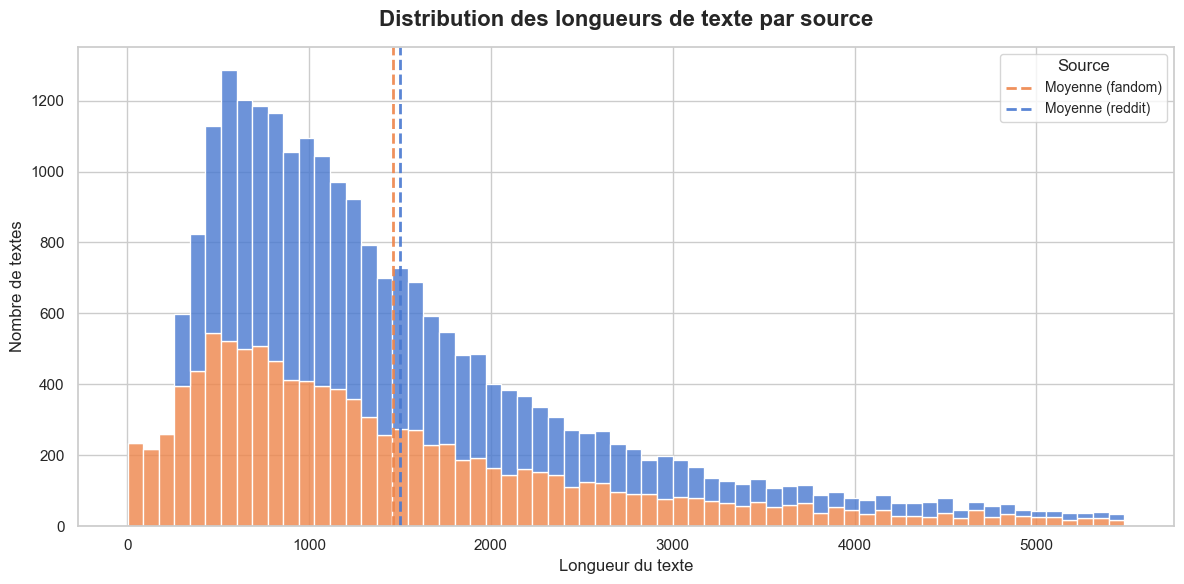
\includegraphics[width = 0.7\textwidth]{illustration/hist_nombre_mots_cp.png}
        
		\caption{Répartition des tailles des productions dans le corpus, en fonction de la plateforme d'origine}
	\end{figure}

	Avec une médiane à 1215 mots et une moyenne à 1816 mots tout corpus confondu, les productions des différentes plateformes sont relativement courtes : à titre de comparaison, un roman, en moyenne, contient entre 50 000 et 100 000 mots.

    % Insérer graohe comparaison taille roman  et fanfic
        	\begin{figure}[htbp]
		\centering
		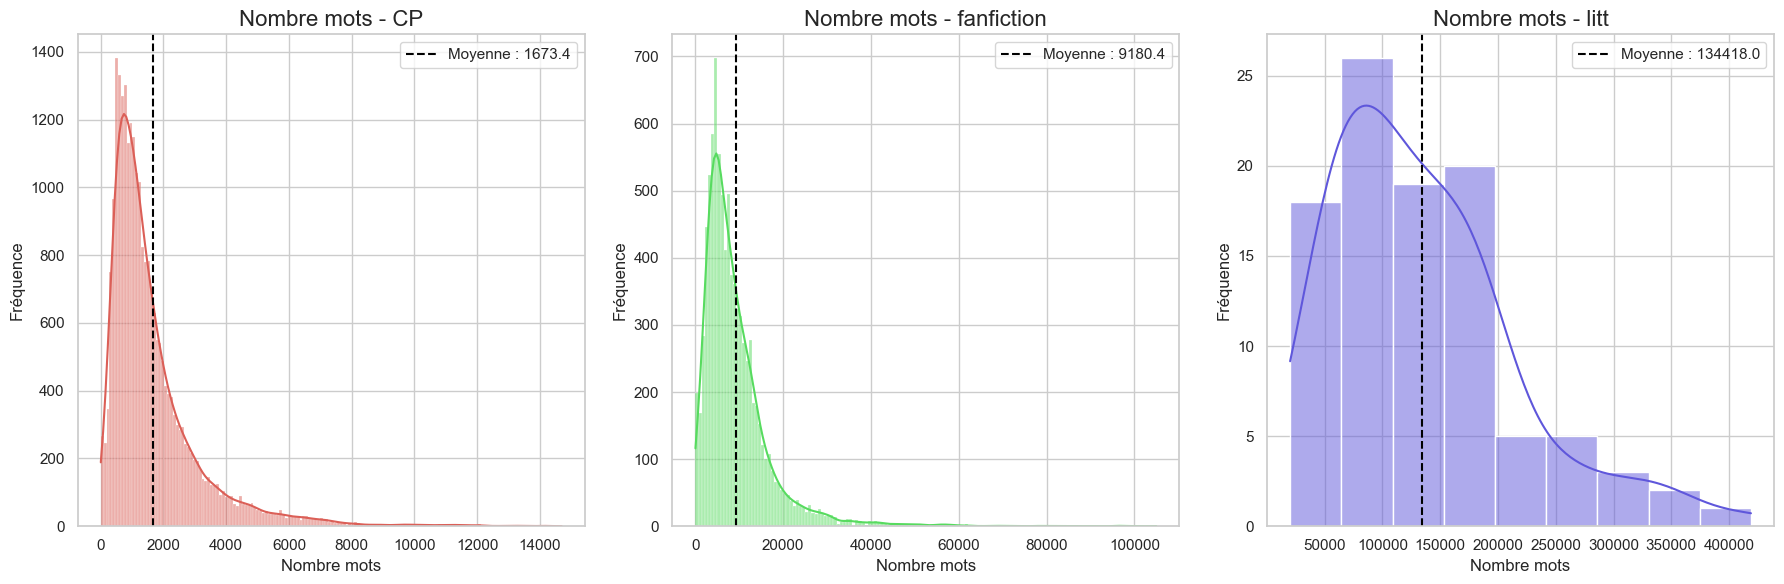
\includegraphics[width = \textwidth]{illustration/nombre_mot_comparaison_sans_abberantes.png}
        
		\caption{Répartition des tailles des productions dans le corpus, en fonction de la plateforme d'origine}
	\end{figure}
	Concernant les deux plateformes, on ne note pas de différence significative : elles semblent être relativement homogènes. 

Afin de mettre plus encore en perspective la taille de ces productions, il peut être intéressant de noter le temps nécessaire pour parcourir une de ces histoires. Le temps de lecture est une métrique intéressante à prendre en compte car plus que le volume de contenu consommé en ligne, c'est le temps passé à consommer ce contenu qui est mesuré. Prenons par exemple les rapports annuels du CNL\footnote{\url{https://centrenationaldulivre.fr/donnees-cles/les-francais-et-la-lecture-en-2025}} concernant la lecture :  le constat que les français lisent moins est étayé par la baisse du temps consacré à la lecture, et non le volume de livres consommé. 

D'après une méta-analyse de 2019 \footcite{BRYSBAERT2019104047}, la vitesse de lecture silencieuse moyenne de fiction pour un lecteur anglophone est comprise entre 200 et 320 mots par minute. 
Rapporté à la taille moyenne des CP, il faut entre 5,75 et 9,08 minutes en moyenne pour lire une de ces histoires. 
Cette rapidité de consommation de contenu, si elle est part d'une évolution plus globale de la production et consommation de contenu en ligne, permet de quantifier à la fois la faible longueur et d'affirmer l'hypothèse d'un contenu visant à se propager plus facilement. 


Autre élément qu'il est intéressant d'analyser, la longueur moyenne des phrases. Cet élément est souvent associé à la littérarité : plus la phrase est longue, plus la phrase peut être complexe. 

    \begin{figure}[htbp]
    \centering
    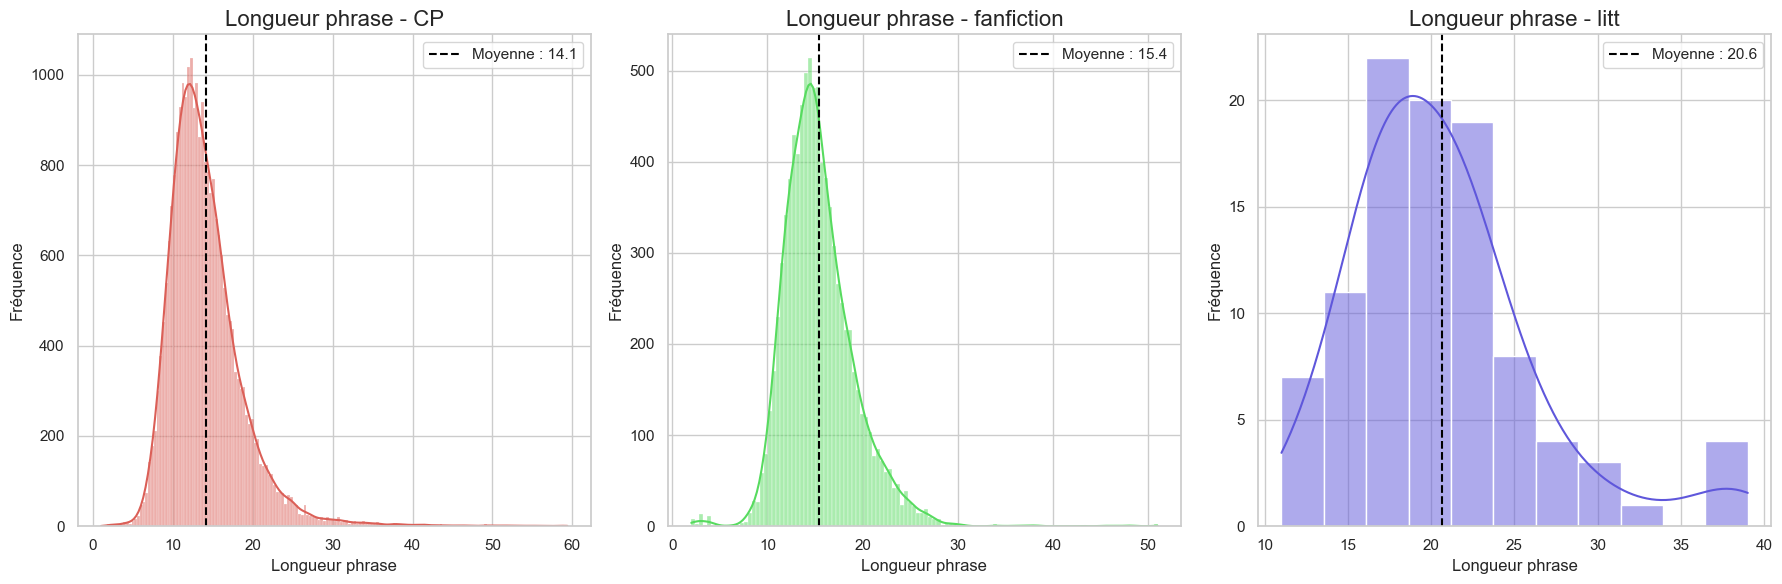
\includegraphics[width = \textwidth]{illustration/longueur_phrase_comparaison_sans_abberantes.png.png}
    \caption{Comparaison de la dispersion des longueurs moyenne des phrases en fonction des corpus}
\end{figure}
	
Nous pouvons rapidement remarquer que, si les creepypastas et fanfictions ont une distribution relativement similaire et une moyenne quasiment identique,\footnote{Voici, à titre de comparaison, une phrase de 15 mots : \texttt{Lorem ipsum dolor sit amet, consectetur adipiscing elit. Nullam at cursus felis, quis posuere nisi.}} les productions littéraires brillent par des phrases significativement plus longues. Ce constat va dans le sens de l'hypothèse précédemment évoquée, appliquée cette fois à une littérature en ligne plutôt qu'au CP spécifiquement.

Au vu des constats précédents, il peut être intéressant de vérifier l'évolution de la taille moyenne des phrases lorsque le texte augmente.  

L'examen des graphiques de régression (\ref{fig:reg2_source} )révèle une relation complexe et non linéaire entre la taille du texte et la longueur moyenne des phrases, ne permettant pas d'affirmer une évolution corrélée entre les deux variables. Les Creepypastas et fanfictions présentent une dynamique similaire en "U", avec des phrases plus courtes pour les textes de longueur intermédiaire. En contraste, les productions littéraires affichent des phrases globalement plus longues et une tendance majoritairement croissante avec la taille du texte. 
Le graphique combiné (\ref{fig:reg2_corpus}) souligne un point culminant de longueur de phrase pour des textes de taille moyenne, suivi d'un déclin. Ainsi la longueur des phrases semble être dépendante de la source du texte plutôt que de son ampleur.

%% Régression taille / longueur phrase

		\begin{figure}[htbp]
		\centering
		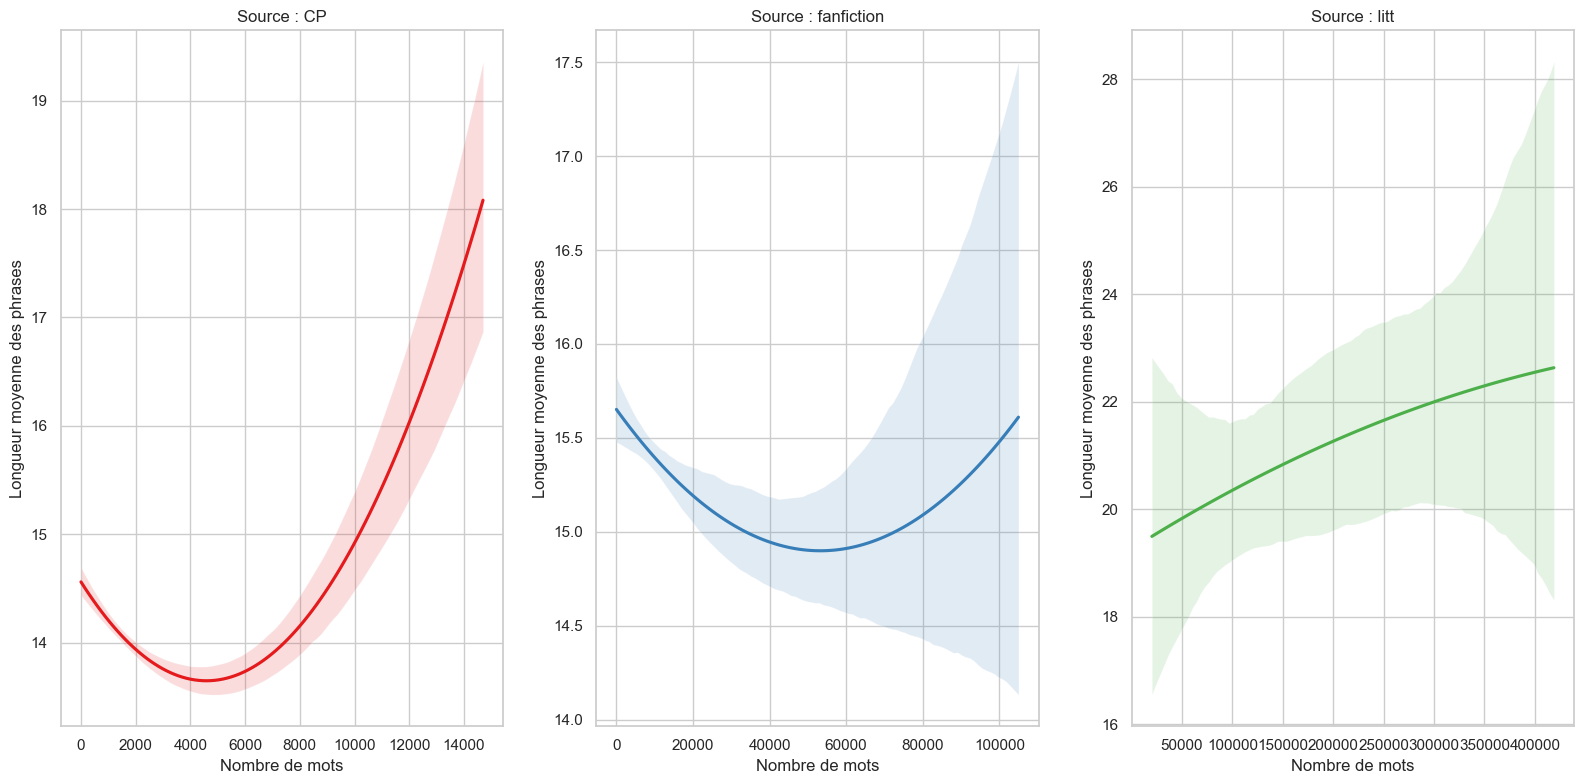
\includegraphics[width = \textwidth]{illustration/reg2_phrases_mots_source.png}
		\caption{Régression polynomiale d'ordre 2 de l'évolution de la longueur moyenne des phrases en fonction du nombre de production, par source}
        \label{fig:reg2_source}
	\end{figure}


    \begin{figure}[htbp]
		\centering
		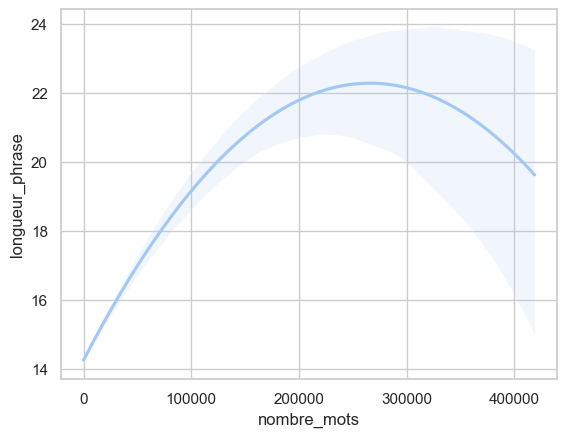
\includegraphics[width = 0.4\textwidth]{illustration/reg2_phrase_mots.png}
		\caption{Régression polynomiale d'ordre 2 de l'évolution de la longueur moyenne des phrases en fonction du nombre de production}
        \label{fig:reg2_corpus}
	\end{figure}
    
%Conclusion
Ainsi il apparaît que c'est avant tout l'aspect numérique qui prévaut pour les phrases : les phrases en lignes plus courtes semblent s'adapter à une nouvelle manière de lire.

La taille, courte en moyenne, des CP semble confirmer l'hypothèse d'une littérature construite pour faciliter la diffusion.

	% richesse lexicale et lisibilité
\section{Mesurer la complexité d'un texte : Richesse Lexicale et indice de lisibilité, syntaxe et perplexité}
	
	Une manière de mesurer le caractère littéraire d'une œuvre réside dans la mesure de sa complexité. Mesurer la complexité d'un texte peut se faire de plusieurs manières. Dans une perspective quantitative, nous avons sélectionné quatre indicateurs : les indices de lisibilité, les indices de richesse lexicale, les indices syntaxiques et la perplexité. 
    Cette combinaison de métriques est aussi bien une application de différentes méthodes utilisées précédemment sur des corpus littéraires dans le cadre d'étude computationnelle, qu'une assurance d'embrasser une gamme large de caractéristiques formelles des textes. 
	Pour rendre l'étude de ces indices plus pertinente, les résultats seront comparés  au corpus de fanfiction et de littérature anglaise. \footnote{Pour les graphiques, la légende sera la même à chaque fois : rouge pour la littérature, vert pour les fanfictions, et bleu pour les CP}

	\subsection{Les indices de lisibilités} 
    
	Les indices de lisibilité sont des indices calculés afin de mesurer la difficulté à lire un texte. Le plus souvent, la valeur de ces indices est associée à un niveau scolaire : en effet, ces indices sont souvent un moyen de rendre compte de la difficulté d'un texte dans le cadre pédagogique. Si ces indices ont des défauts (que chacun essaye de corriger vis-à-vis d'un autre indice), ils permettent néanmoins de rendre compte de mécanisme syntaxiques qui statistiquement rende le texte plus difficile à parcourir.
	En ce qui nous concerne, notre but est d'une part de caractériser la lisibilité des CP, tout en rendant compte de la difficulté relative de lecture. Comme nous l'avons mentionné précédemment, nous faisons l'hypothèse d'une lisibilité relativement élevée, en lien avec une prétention grandissante à la littérarité.
	
	\begin{figure}
\centering
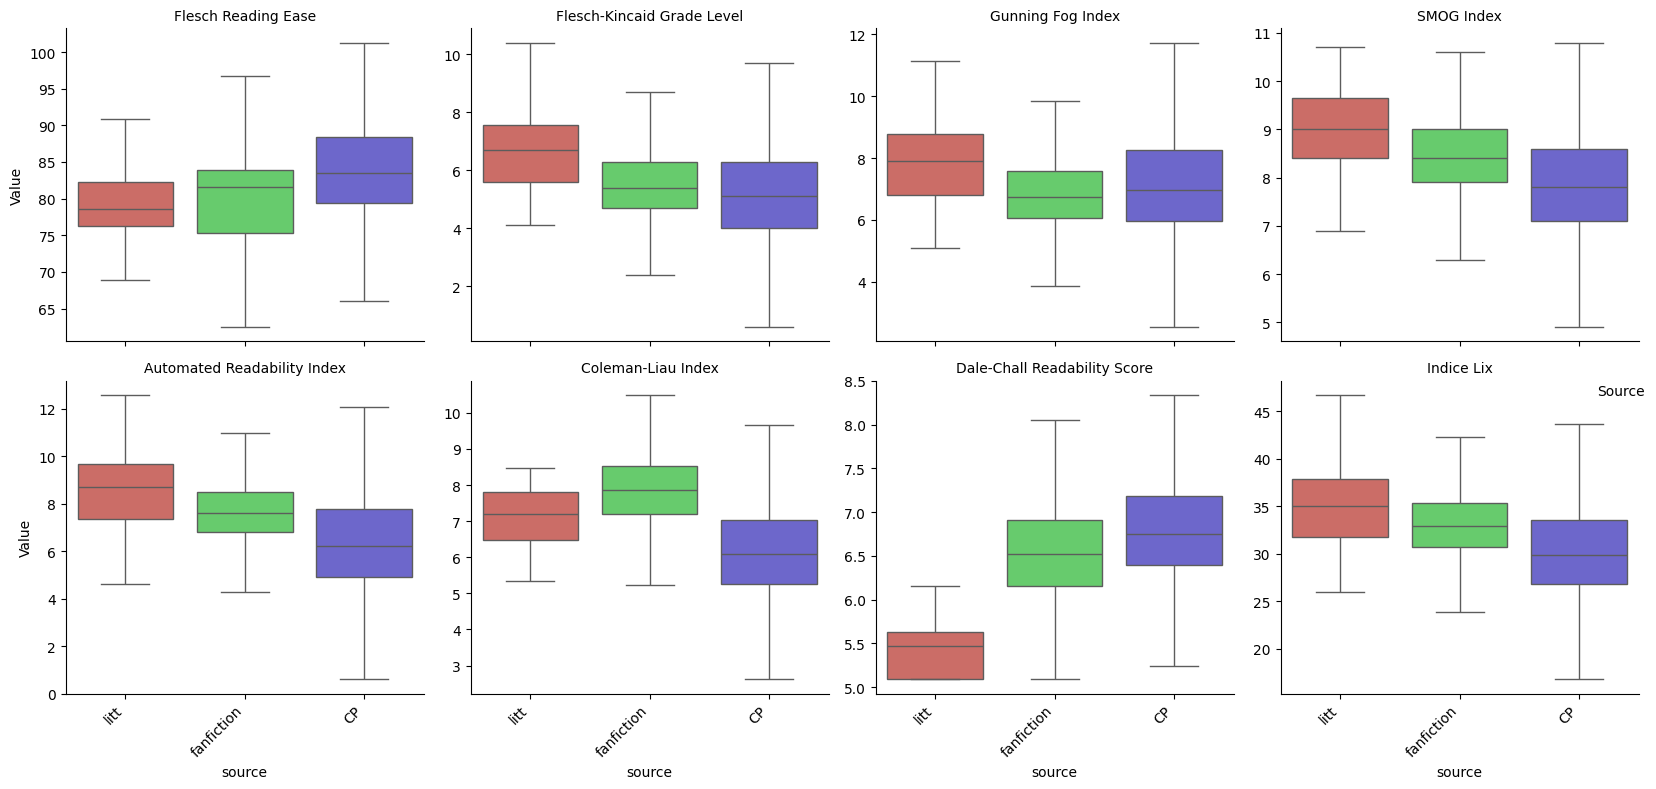
\includegraphics[width = \textwidth]{illustration/readability_per_source.png}
\caption{Moyenne des indices de lisibilités sur le corpus}
\label{fig:mean_readbility}
	\end{figure}
	
	Avant de comparer les résultats, il convient d'analyser les valeurs de ces indices. Pour celles-ci, les valeurs correspondent au niveau scolaire théorique adapté pour la lecture dudit texte. Plus l'indice est haut, plus le texte est exigeant. Pour les équivalences entre les valeurs et le niveau scolaire, voir les tables \ref{tab:readability_indices_part1} et \ref{tab:readability_indices_part2}.
	

	Pour ce qui est des valeurs, on note pour tous les indices des valeurs basses, du moins plus basses que ce à quoi on pourrait s'attendre d'un genre littéraire (cf. Figure \ref{fig:mean_readbility}): Les indices oscillent entre un niveau scolaire primaire et secondaire, soit des textes accessibles à des jeunes collégiens.


Les résultats des différents indices de lisibilité mettent en lumière des différences nettes entre les trois types de corpus analysés : littérature, fanfiction et creepypasta. 

Globalement, les creepypastas apparaissent comme les textes les plus faciles à lire, avec des scores plus élevés au Flesch Reading Ease et plus faibles aux autres indices de complexité comme le Gunning Fog Index, le SMOG ou l’Automated Readability Index.

À l’inverse, la littérature classique tend à présenter une plus grande complexité lexicale et syntaxique, en particulier selon les indices sensibles à la longueur des phrases (Fog, Lix) ou au niveau scolaire requis (Flesch-Kincaid, ARI), bien que certaines œuvres littéraires utilisent un vocabulaire relativement accessible, ce qui explique leur score faible au Dale-Chall. 

La fanfiction occupe une position intermédiaire, mais se distingue par une certaine hétérogénéité : elle tend à utiliser un lexique plus spécialisé (cf. Coleman-Liau), tout en conservant des structures syntaxiques plus simples que la littérature. 

Les résultats montrent donc que les creepypastas se distinguent par une lisibilité nettement supérieure à celle des textes littéraires et des fanfictions. Les indices Flesch, Flesch-Kincaid, Gunning Fog et SMOG convergent vers une écriture simple, caractérisée par des phrases courtes et un vocabulaire accessible. 
%Cette clarté syntaxique semble répondre aux contraintes du support numérique et à l’objectif de captation rapide du lecteur.

    
		
	\begin{figure}
		\centering
		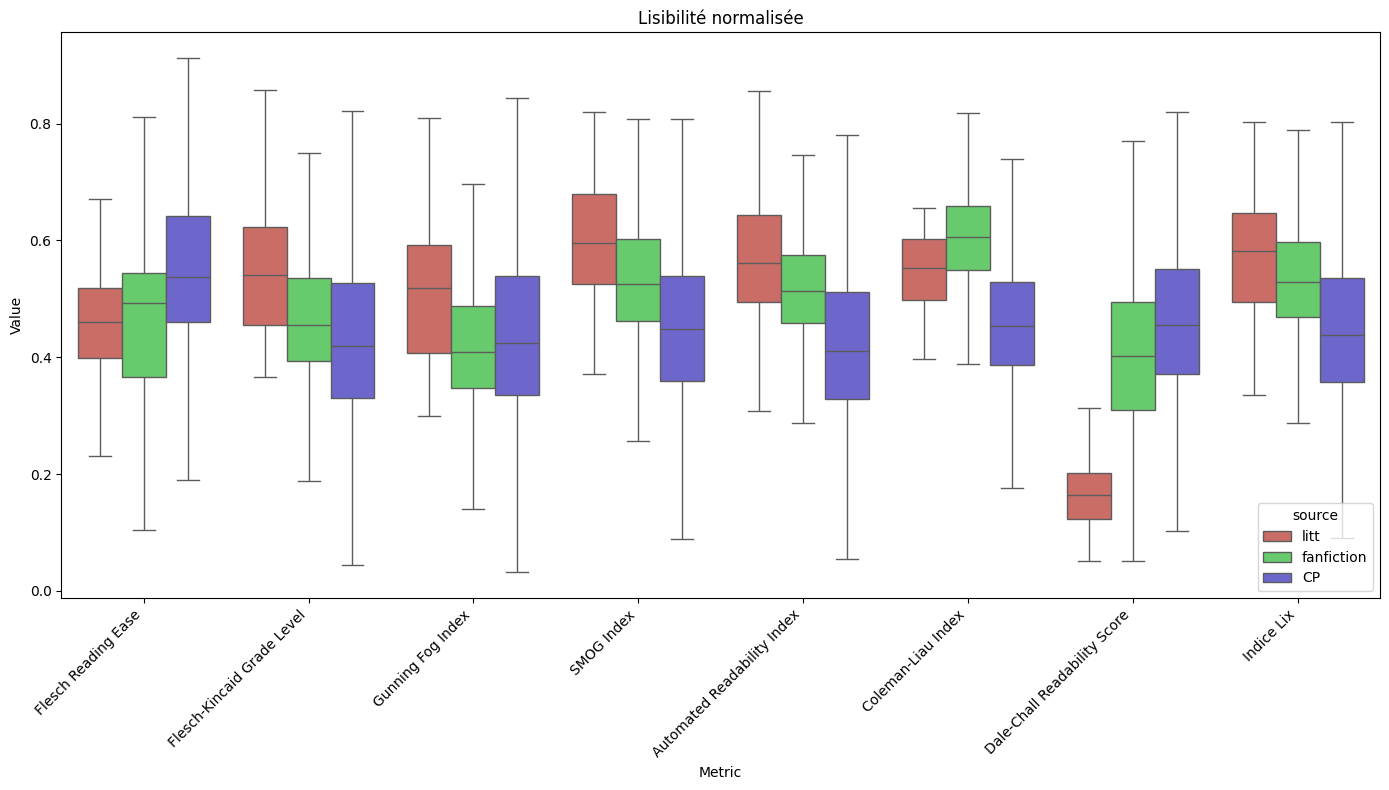
\includegraphics[scale=0.45]{illustration/readabiliy_norm.png}
		\caption{Comparaison des indices de lisibilités normalisés entres les différentes sources}
		\label{fig:comparaison_readability}
	\end{figure}
	
\pagebreak
	
	
	%Comparaison des richesse lexicales 
\subsection{Les indices de richesse lexicales}

Allant de pair avec la difficulté de lecture, les indices des mesures lexicales sont, comme leur nom l'indique, des mesures de la richesse du vocabulaire. Bien que chaque indice fonctionne différemment (cf. Partie \ref{annexe_richesse_lex}), le principe reste similaire : on compare le nombre total de mots ou de tokens à un élément spécifique. Nous avons sélectionné initialement quatre indices (cf. \ref{annexe_richesse_lex}).

Comment mentionné durant l'introduction, le point d'entrée de cette étude en matière de richesse lexicale est l'étude d'Algee Lewit\footcite{algee2016canon}. Néanmoins, le TTR n'est pas sans inconvénient : du fait de sa construction, cet indice est fortement corrélé à la taille du texte. Ainsi, pour palier à ce problème, nous avons appliqué une variante de celui-ci, le Moving Average TTR \footcite{covington2010cutting}, qui contourne le problème de la taille en calculant une moyenne de l'indice sur des extraits successifs du texte. Néanmoins, dans un souci de lisibilité, nous continuerons de mentionner le TTR au cours des analyses.

Ces indices mettent en évidence des dynamiques contrastées entre les trois types de textes (\ref{fig:richeness_source}. Le ratio types/tokens, indicateur classique de la richesse lexicale, révèle une valeur légèrement supérieure dans les fanfictions, suivies de près par les textes littéraires, tandis que les creepypastas présentent des scores un peu plus faibles. Cette tendance est confirmée par l’indice de densité lexicale, qui évalue la proportion de mots pleins dans le texte : les fanfictions affichent ici également une densité supérieure, témoignant d’un style plus informationnel.

Les résultats relatifs aux hapax legomena, c’est-à-dire les mots n’apparaissant qu’une seule fois dans le corpus, renforcent cette observation. Les textes littéraires se démarquent nettement par un nombre plus élevé d’hapax, suggérant une plus grande inventivité lexicale ou une plus grande hétérogénéité de style. À l’inverse, les creepypastas en comptent très peu, ce qui témoigne d’une forte redondance lexicale ou d’un lexique plus restreint.

Enfin, l’indice de Honoré (R), qui combine fréquence des hapax et volume total, confirme globalement ce classement : les textes littéraires et les fanfictions présentent une richesse lexicale comparable, légèrement supérieure à celle des creepypastas, même si les écarts sont ici moins marqués. Ce résultat souligne que, si les creepypastas se caractérisent par une lisibilité plus grande, cela se fait au prix d’une réduction sensible de la diversité lexicale.

Dans l'ensemble, les creepypastas présentent une diversité lexicale plus faible. Le nombre d’hapax, la densité lexicale, le ratio types/tokens et l’indice de Honoré indiquent un vocabulaire plus restreint que dans les autres corpus. 

\begin{figure}
    \centering
    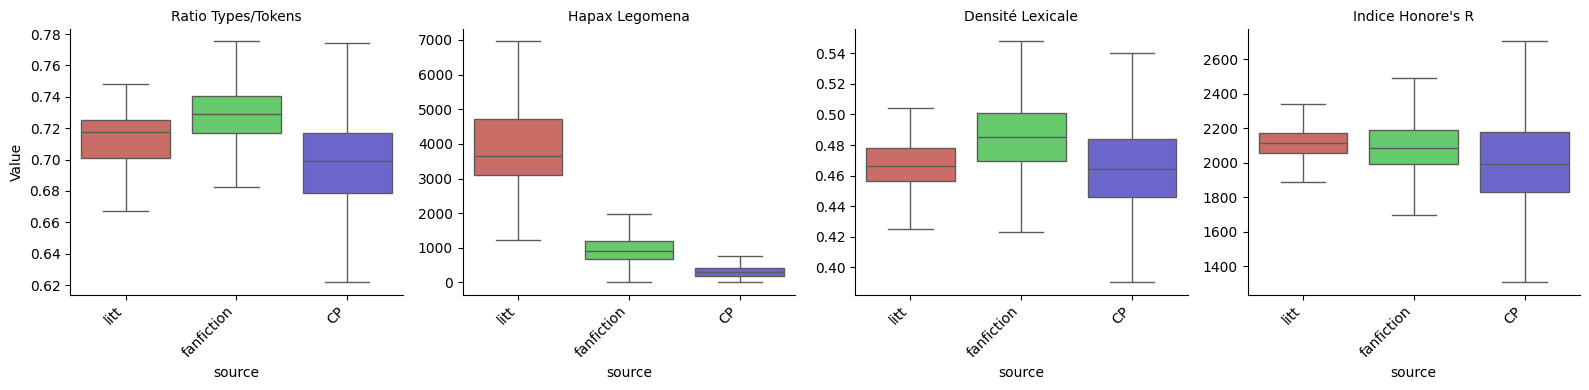
\includegraphics[width=0.5\linewidth]{illustration/richness_per_source.png}
    \caption{Distribution des indices de richesse lexicale en fonction de la source}
    \label{fig:richeness_source}
\end{figure}

\begin{figure}
    \centering
    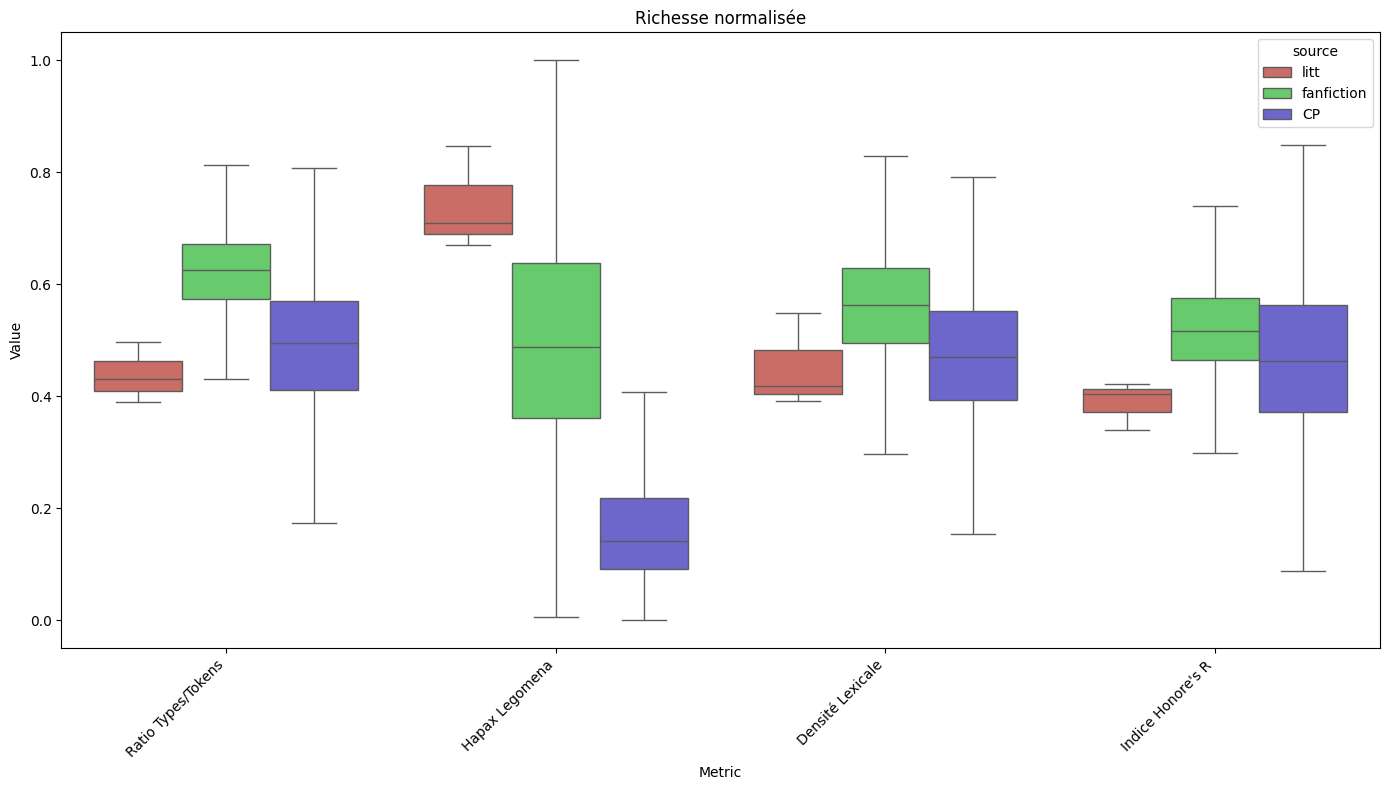
\includegraphics[width=0.5\linewidth]{illustration/richness _norm.png}
    \caption{Distributions des indices de richesse lexicale en fonction de la source, normalisés}
    \label{fig:richness_norm}
\end{figure}



\subsection{Complexité syntaxique}
%Ration nom/verbes + verbe passif + ratio nom+ adj / verbe voie passive

Une autre approche à la question de la littérarité est celle du style, du moins de la syntaxe associée. L'idée derrière la complexité syntaxique est de mettre en avant des éléments de syntaxe plus rares dans des productions moins littéraires, comme le style nominal, ou l'utilisation de la voie passive. 
Contrairement aux approches principalement lexicométriques sur lesquelles reposent la lisibilité et la richesse lexicale, l'approche syntaxique repose sur la détection préalable des natures grammaticales des mots. Pour ce faire, nous avons privilégié une approche automatique, à l'aide d'un modèle SpaCy (\texttt{en\_core\_web\_sm}). 

\begin{figure}
    \centering
    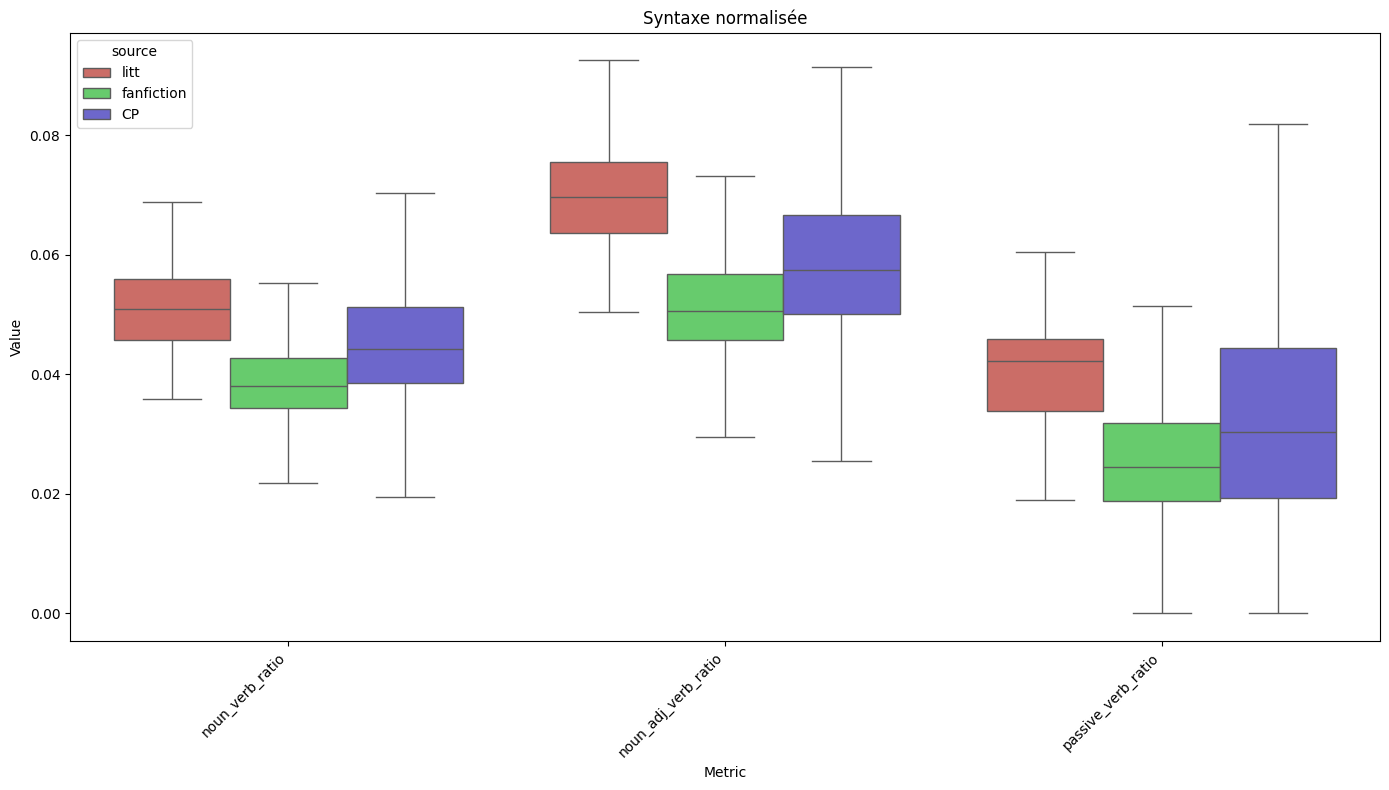
\includegraphics[width=0.5\linewidth]{illustration/synt_norm.png}
    \caption{Comparaisons des trois métriques syntaxiques retenues (normalisées)}
    \label{fig:complexe_norm}
\end{figure}
On remarque assez rapidement que les métriques du corpus littéraire sont systématiquement supérieures à celles des autres corpus(\ref{fig:complexe_norm}) : aussi bien la médiane que les valeurs minimales  (<Q1). Ainsi le corpus littéraire emploie a priori un style plus nominal et la voie passive plus abondamment. 

En revanche , la comparaison entre les corpus numériques est peut-être plus surprenante : ce sont les CP qui apparaissent comme utilisant un style plus littéraire. 

Le style nominal est associé à un style plus descriptif, plus abstrait, là où un style verbal est associé à l'action et la progression du récit.
Sachant cela, les conclusions que l'on peut tirer de la distribution de ces indices vont finalement dans le sens de l'esthétique des CP décrite jusqu'ici. Le narrateur est souvent soit victime soit témoin d'une situation qu'il ne maîtrise pas, d'où une utilisation plus importante de la voie passive, retranscription syntaxique de cette passivité (on note que même si la médiane est plus faible, l'étalement des valeurs est plus important, avec un >Q3 très élevé).
Le style plus nominal va dans ce même sens : les CP, afin de transmettre le sentiment de peur, se doivent de prendre le temps de la description, élément que le style nominal favorise. 

À l'inverse, nous pouvons émettre l'hypothèse que les fanfictions s'appuient sur un rythme de récit plus soutenu, marqué par une progression narrative plus importante. Les principales fanfictions s'appuient sur des œuvres d'aventures, de fantasy ou d'action \footnote{Les fandom les plus représentés sur le site \textit{AO3} sont Harry Potter, le shonen \textit{My Hero Academia}, ou encore l'univers de superhéros Marvel} favorisant ainsi un style moins abstrait.



\subsection{Perplexité}


La dernière méthode employée pour mesurer la complexité textuelle s'appuie sur l'utilisation d'un modèle de langue et, plus précisément, sur le calcul de la perplexité. Cette approche, suivant les travaux de Wu et al.\footcite{wu2024perplexing}, permet de quantifier la "surprise" linguistique générée par l'enchaînement des mots au sein de différents corpus. En effet, la perplexité constitue une mesure probabiliste qui évalue dans quelle mesure un modèle de langue parvient à prédire la séquence de tokens observée : plus la perplexité est élevée, plus le texte est imprévisible et donc complexe du point de vue du modèle.

Soit une séquence tokenisée \( X = (x_0, x_1, \dots, x_t) \). La perplexité de \( X \), notée \( \text{PPL}(X) \), est définie par :

\[
\text{PPL}(X) = \exp\left( -\frac{1}{t} \sum_{i=1}^{t} \log p_\theta(x_i \mid x_{<i}) \right)
\]

où \( p_\theta(x_i \mid x_{<i}) \) désigne la probabilité, estimée par un modèle paramétré par \( \theta \), du token \( x_i \) sachant les tokens précédents \( x_{<i} \).

\begin{figure}
    \centering
    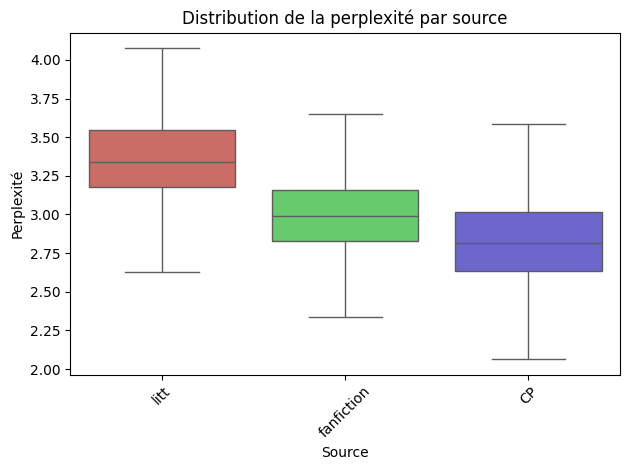
\includegraphics[width=0.5\linewidth]{illustration/perplexity_source.png}
    \caption{Distribution de la perplexité en fonction de la source}
    \label{fig:perplexity}
\end{figure}

Cette mesure repose sur le principe que la complexité d'un texte peut être appréhendée à travers la difficulté qu'éprouve un modèle de langue pré-entraîné à prédire chaque token successif. \footnote{Voir ici pour la méthode en détail et le code utilisée :\url{https://huggingface.co/docs/transformers/perplexity}}

L'analyse comparative révèle une hiérarchisation nette de la perplexité entre les trois corpus étudiés (Figure \ref{fig:perplexity}). Les textes littéraires présentent la perplexité la plus élevée témoignant d'une sophistication stylistique qui rend leur prédiction plus ardue en comparaison pour le modèle. La fan-fiction occupe une position intermédiaire , mais se caractérise par une variabilité accrue, reflétant l'hétérogénéité des pratiques d'écriture amateur. Enfin, les creepypastas affichent la perplexité la plus faible accompagnée de la plus forte dispersion, suggérant l'existence de formules narratives récurrentes propres à ce genre populaire en ligne. 


\subsection{Conclusion sur la complexité des textes}

L'analyse comparative de la complexité textuelle à travers quatre dimensions méthodologiques suggère une configuration plus nuancée qu'il n'y paraît au premier abord. Si les mesures convergent généralement vers une hiérarchisation attendue — littérature canonique en tête, creepypastas en position apparemment moins complexe —, l'examen détaillé révèle des dynamiques plus subtiles qui méritent d'être soulignées.

Les creepypastas, au cœur de cette étude, présentent un profil ambivalent qui interroge nos conceptions traditionnelles de la complexité littéraire. D'un côté, ces textes semblent effectivement privilégier l'accessibilité : indices de lisibilité élevés, vocabulaire moins diversifié, perplexité relativement faible. Cette simplicité apparente pourrait s'expliquer par les contraintes du support numérique et l'objectif de captation immédiate du lecteur. Cependant, l'analyse syntaxique révèle une image plus contrastée : les creepypastas mobilisent des stratégies stylistiques spécifiques — style nominal marqué, usage de la voix passive — qui témoignent d'une recherche esthétique particulière.

Cette apparente contradiction invite à reconsidérer la nature même de la complexité dans les productions numériques populaires. Les creepypastas semblent développer une forme de sophistication ciblée, adaptée aux exigences du genre horrifique : la construction de l'atmosphère, la suggestion de l'indicible, la création d'une tension narrative spécifique. Cette complexité, bien que différente de celle de la littérature canonique, n'en demeure pas moins réelle et fonctionnelle.

Les fanfictions, pour leur part, confirment leur statut intermédiaire, oscillant entre héritage littéraire et contraintes numériques. Elles témoignent de la diversité des pratiques d'écriture amateur, entre appropriation créative et reproduction de formules établies.

Cette étape suggère ainsi que la complexité textuelle ne saurait être réduite à une échelle unidimensionnelle, elle invite plutôt à envisager des formes plurielles de sophistication littéraire, chacune répondant à des objectifs esthétiques et à des contraintes génériques spécifiques. Pour les creepypastas, cette complexité semble résider moins dans la virtuosité lexicale que dans la maîtrise de codes narratifs et stylistiques propres à la production de l'effet recherché.

\section{ Analyse thématique et affective}
La précédente partie a permis de montrer que, malgré une accessibilité accrue, les creepypastas développaient un dispositif stylistique spécifique.


	\subsection{Modélisation de sujet}
	\label{section_topic}


Afin de caractériser au mieux les productions, un bon moyen est d'identifier puis d'analyser les thèmes les plus fréquents. Comme nous l'avons mentionné précédemment, les CP se démarquent à la fois par leur forme et par leurs thèmes précis (numérique, vie de tous les jours...). Ainsi, cette analyse va nous permettre de vérifier cette hypothèse à l'échelle du corpus et non pas quelques exemples marquants. 

Notre démarche méthodologique vise à faire émerger, sans supervision préalable, les principales communautés thématiques structurant notre corpus. Contrairement aux classifications manuelles imposant des catégories exogènes, nous privilégirons l'émergence endogène des structures thématiques à partir des propriétés lexicales des textes, limitant ainsi les biais interprétatifs inhérents aux taxonomies préétablies.

\subsubsection{Construction des représentations textuelles par TF-IDF}

La transformation du corpus en vecteurs exploitables repose sur la méthode TF-IDF, dont la pertinence épistémique réside dans sa double pondération : fréquence locale des termes (TF) et leur rareté relative dans l'ensemble documentaire (IDF). 
Le processus comprend :
\begin{itemize}
    \item L'application de la formule TF-IDF classique : $TF\text{-}IDF(t,d) = TF(t,d) \times IDF(t)$
    \item Un prétraitement lexical incluant l'élimination des mots fonctionnels, la suppression des marqueurs techniques artéfactuels, et l'établissement d'une liste d'exclusion enrichie
\end{itemize}

\subsubsection{Élaboration du graphe de similarité textuelle}

La matrice de similarité cosinus, calculée entre les vecteurs TF-IDF, permet d'établir la proximité sémantique entre documents indépendamment de leur longueur. L'application d'un seuil critique, déterminé empiriquement, transforme cette matrice en graphe non orienté et pondéré où :
\begin{itemize}
    \item Les nœuds représentent les documents
    \item Les arêtes symbolisent les similarités significatives
    \item Les poids correspondent aux valeurs de similarité
\end{itemize}

Ce graphe non orienté est généré grâce à la version python du paquet \textit{iGraph} \footcite{Csardi_The_igraph_software_2006}. L'essentiel des computations opérées sur le graphique s'appuie sur les options disponibles dans celui-ci.

\subsubsection{Optimisation structurelle et détection algorithmique}

Deux opérations critiques précèdent l'identification communautaire :
\begin{enumerate}
    \item L'élimination des boucles réflexives non-informatives
    \item L'extraction de la composante connexe principale via la méthode \texttt{.giant()}
\end{enumerate}

Cette dernière opération, bien que pouvant sembler restrictive, se justifie par la concentration sur le cœur sémantique du corpus et l'amélioration conséquente de la robustesse algorithmique.

La détection communautaire proprement dite mobilise l'algorithme de Leiden\footcite{Traag2019}, optimisation de l'algorithme de Louvain, qui opère par maximisation de la modularité :

\begin{equation}
Q = \frac{1}{2m}\sum_{i,j} \left[ A_{ij} - \frac{k_i k_j}{2m} \right] \delta(c_i, c_j)
\end{equation}

Cet algorithme présente l'avantage décisif d'intégrer naturellement la pondération des arêtes, transposant ainsi la force des similarités textuelles dans le processus de partitionnement. La partition obtenue émerge de la structure même du graphe, sans paramétrage a priori du nombre de communautés attendues.

\subsubsection{Interprétation sémantique des communautés}

L'identification structurelle des communautés nécessite une herméneutique complémentaire pour révéler leur signification thématique. Pour chaque communauté, nous calculons :
\begin{enumerate}
    \item Le vecteur TF-IDF moyen par agrégation des vecteurs documentaires individuels
    \item Les termes aux scores TF-IDF moyens les plus élevés, constituant la signature lexicale de la communauté
\end{enumerate}

Les communautés ainsi caractérisées constituent une cartographie des articulations conceptuelles majeures du corpus, révélant potentiellement des structures de sens que les catégorisations préétablies auraient occultées.

\subsubsection{Limites et perspectives critiques}

Notre approche, malgré ses avantages épistémiques considérables, présente certaines limitations qu'il convient d'expliciter :
\begin{itemize}
    \item Le seuil de similarité conserve une dimension partiellement arbitraire influençant la granularité communautaire
    \item L'extraction de la composante principale exclut des documents potentiellement significatifs mais structurellement marginaux
    \item L'interprétation sémantique par extraction lexicale peut occulter des phénomènes plus subtils comme la polysémie
\end{itemize}

Ces limitations constituent moins des invalidations méthodologiques que des invitations à une interprétation nuancée des résultats et à l'élaboration de protocoles complémentaires permettant d'en vérifier la robustesse.

\subsubsection{Analyse des résultats}

	Par cette méthode,  nous avons isolé les thèmes suivants (cf. Figure \ref{fig:topic_corpus}) : 
	\begin{itemize}
		\item la famille et l'enfance
		\item les transports 
		\item la forêt et la nature
		\item la famille proche
		\item la technologie 
		\item citation ancienne et formelle (*)
		\item le corps et les sensations
		\item l'école et l'enfance
		\item les rêves et le sommeil
		\item la vengeance (*)
		\item les miroir et les rituels
		\item le milieu médical
        \item les animaux domestiques
        \item html et artéfacts
        \item les livres et la lecture
        \item l'art et la peinture
        \item la détresse physique et mentale (*)
        \item code machine et paramètres (*)
        \item le désespoir et tragédie (*)
        \item mariage militaire (*)
        \item monstruosité (*)\\

		\end{itemize} 
Une fois les thèmes artéfactuels retirés (*), on remarque la présence des thèmes que nous avons évoqués tout au long de notre caractérisation théorique: la technologie et les jeux-vidéos et l'enfance à travers la famille à plusieurs reprises. D'autres thèmes néanmoins sont peut-être moins attendus, plus surprenants, pour des productions à vocation horrifique, l'importance de la famille par deux thèmes distincts ou bien les animaux de compagnie particulièrement est remarquable. 
    
    	Ces thèmes apparaissent comme ayant un point commun : un rapport étroit avec l'expérience personnelle. La famille, la souffrance, et le foyer sont autant d'éléments relevant de l'intime. 
    	De la même façon, le miroir ou la forêt mobilisent un symbolisme assez proche : le miroir, d'abord, est un lieu de révélation, de prise de conscience, voire d'affrontement \footcite[voir p.639, article "Miroir"]{chevalier_dictionnaire_1990}, là où la forêt est un lieu symbole de l'inconscient et de la crainte de celui-ci, comme plus prosaïquement, un lieu de mystère \footcite[voir p.455, article "Forêt"]{chevalier_dictionnaire_1990}


	\begin{figure}[htbp]
	\centering
	\begin{subfigure}{0.45\textwidth}
		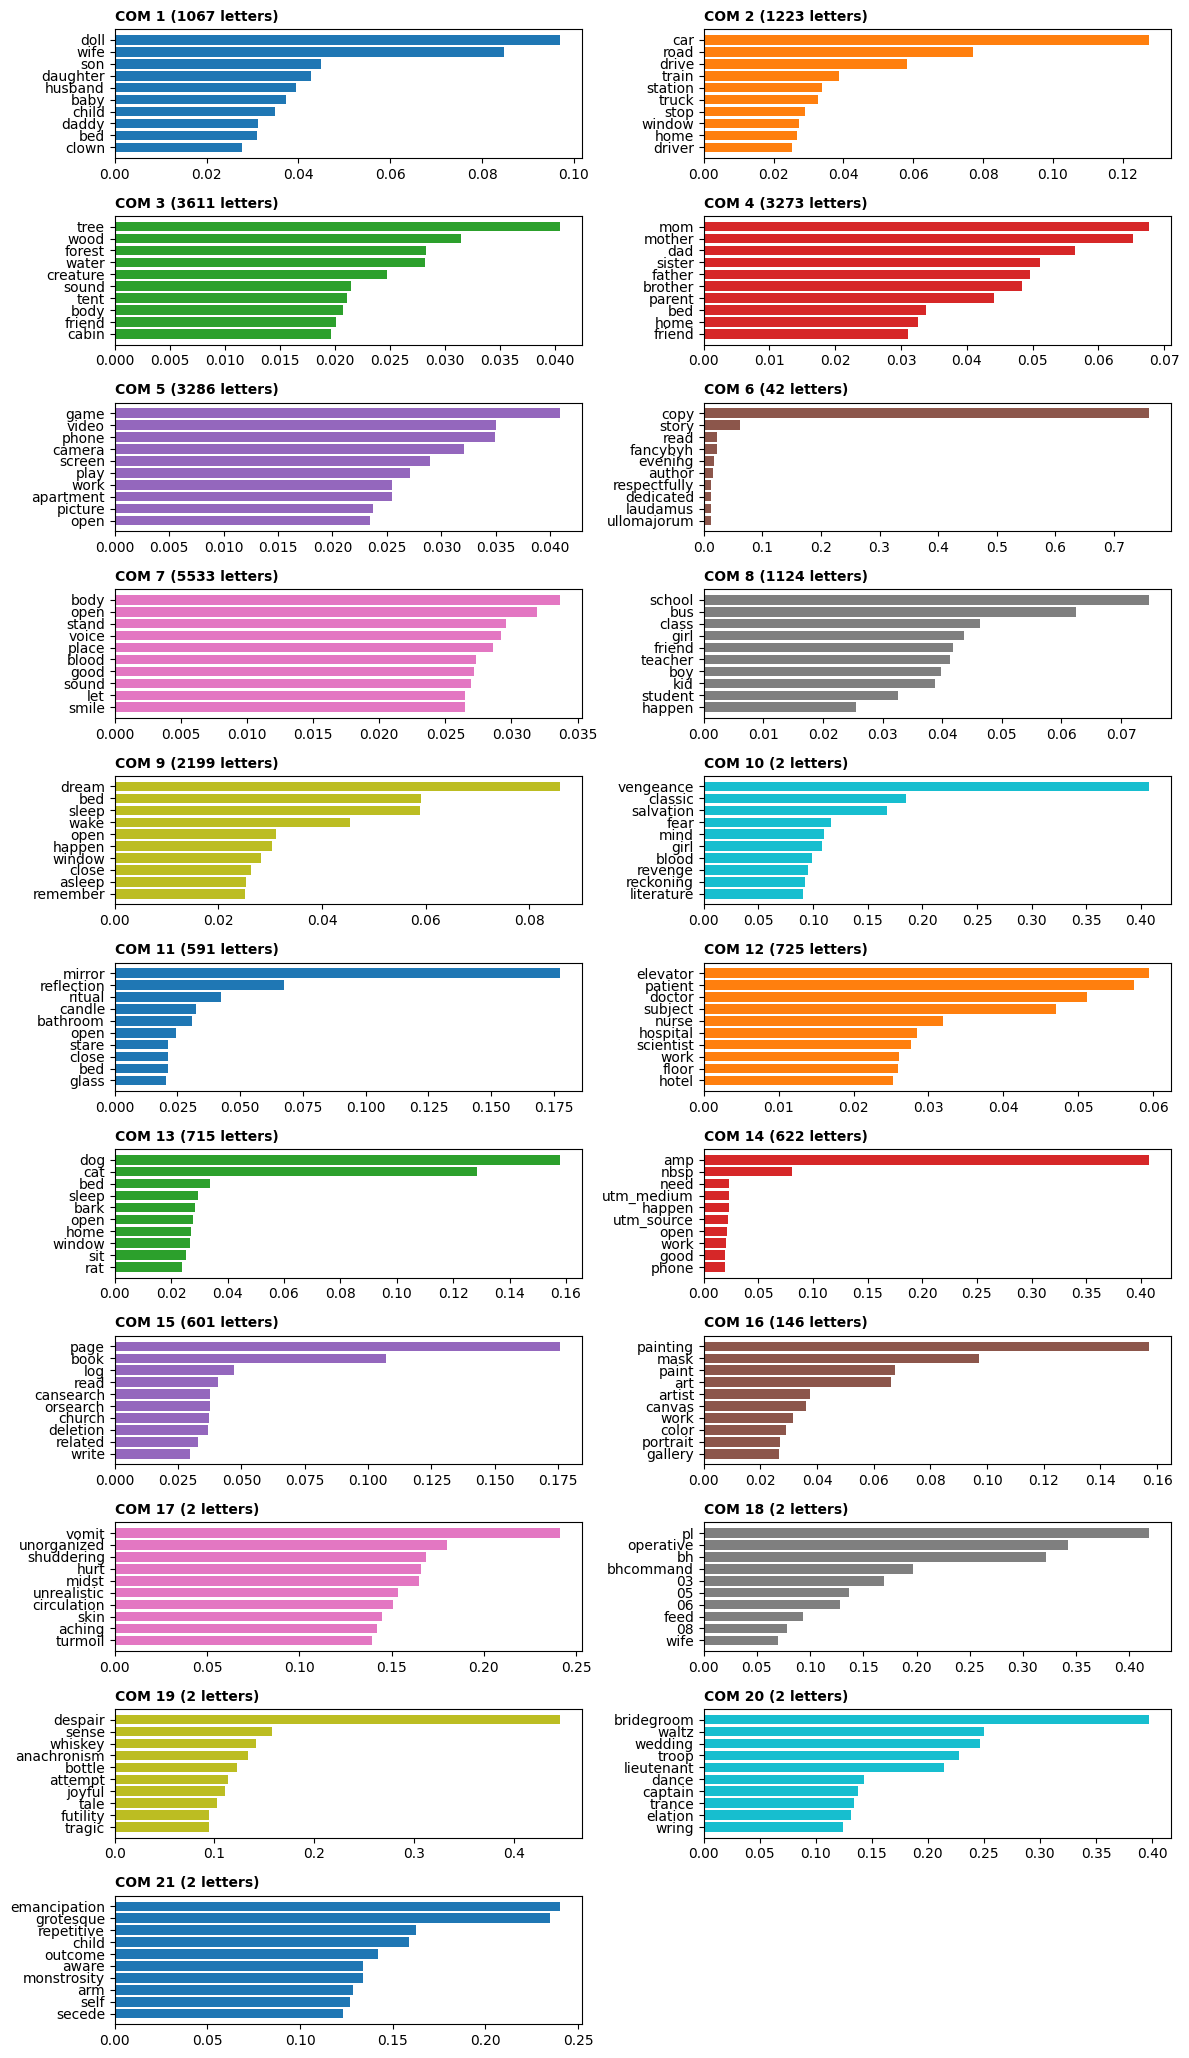
\includegraphics[width=\textwidth]{illustration/topic_corpus.png}
		\caption{Topics les plus fréquents sur l'ensemble du corpus}
		\label{fig:topic_corpus}
	\end{subfigure}
	\hfill
	\begin{subfigure}{0.45\textwidth}
		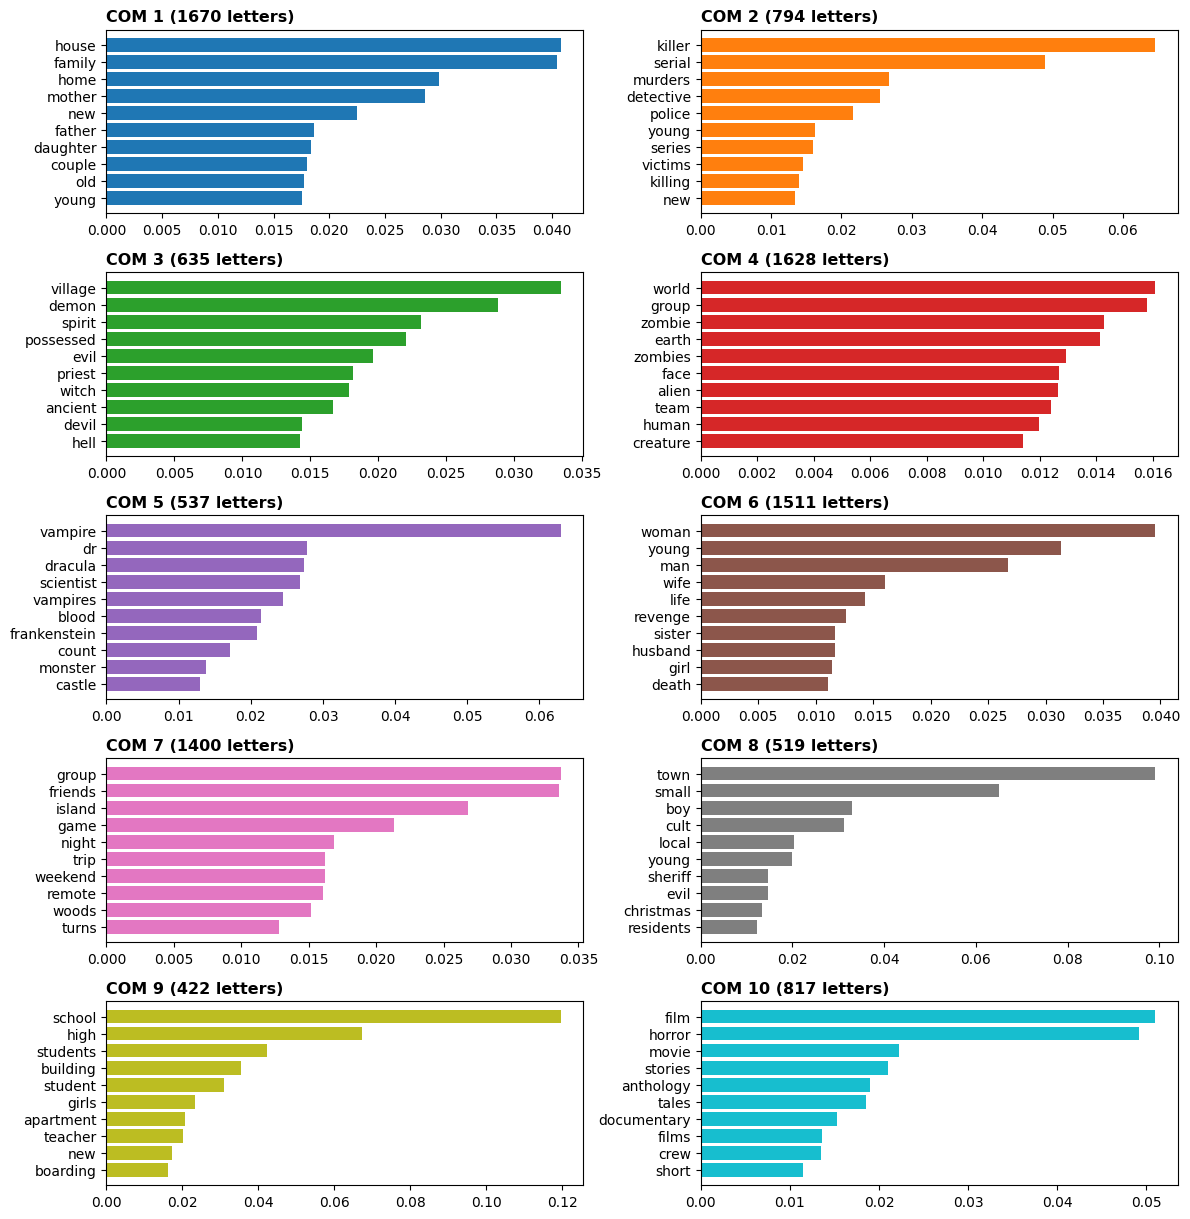
\includegraphics[width=\textwidth]{illustration/topic_tmdb.png}
		\caption{Topics les plus fréquents des films d'horreur de \emph{TheMovieDataBase}}
		\label{fig:topic_tmdb}
	\end{subfigure}
	\caption{Visualisation des topics les plus fréquents de deux corpus de contenu d'horreur}
	\label{fig:topics_corpus}
	\end{figure}
	
	Afin de souligner à quel point ces thèmes sont caractéristiques de ce genre de littérature d'horreur, nous avons cherché à identifier les thèmes les plus récurrents des productions cinématographiques d'horreur.
	Pour ce faire, nous avons suivi la même méthode d'extraction des thèmes cette fois-ci sur un ensemble de descriptions de films d'horreur extrait de la base de données \textit{The Movie Data Base}\footnote{\url{https://www.themoviedb.org/}} (cf. Figure \ref{fig:topic_tmdb}). Ces descriptions ont été obtenues via l'API \footnote{\url{https://developer.themoviedb.org/reference/intro/getting-started}} de la plateforme.
	
	La différence entre les thèmes est flagrante : si les CP évoquent en filigrane l'expérience personnelle, le foyer, l'intimité , les films d'horreur sont plus facilement tournés vers le spectaculaire et le surnaturel (zombie, expérience scientifique, religion, vampire). 
	Ainsi l'hypothèse d'un genre caractérisé par un lien étroit avec l'intimité et l'expérience semble se confirmer : le frisson de l'horreur ne passe que rarement par des effusions de sang, mais bien par quelque chose de plus subtil.
	De plus, les thèmes des CP sont doubles, étant à la fois élément de cadre et potentiellement déclencheurs de la peur. Cette dualité n'est pas présente, ou dans une dimension moindre dans un film d'horreur par exemple . Un zombie, élément déclencheur de la peur par excellence, n'est pas nécessairement un élément cadrant du récit, du moins pas au même titre que la famille par exemple, qui peut aussi bien être un thème cadre, et ce qui, une fois pervertie ou distordues, apporte l'élément horrifique. Dès lors, on peut supposer que la subtilité des thèmes et de l'horreur est double : la peur n'est pas issue d'élément spectaculaire, et elle est présente dans tous les recoins du récit.
    %et  par une présence diffuse, qui infuse donc le récit.

\subsubsection{Cohérences des thèmes à travers les corpus}

Ces hypothèses sont en partie confirmées par les mesures de cohérence des sujets à travers le corpus : la cohérence \footcite{10.1145/2684822.2685324} est une mesure de la pertinence d'un sujet (ou plutôt du sac de mots qui forme le sujet).

\begin{figure}[htbp]
\centering
\begin{subfigure}[b]{0.45\textwidth}
    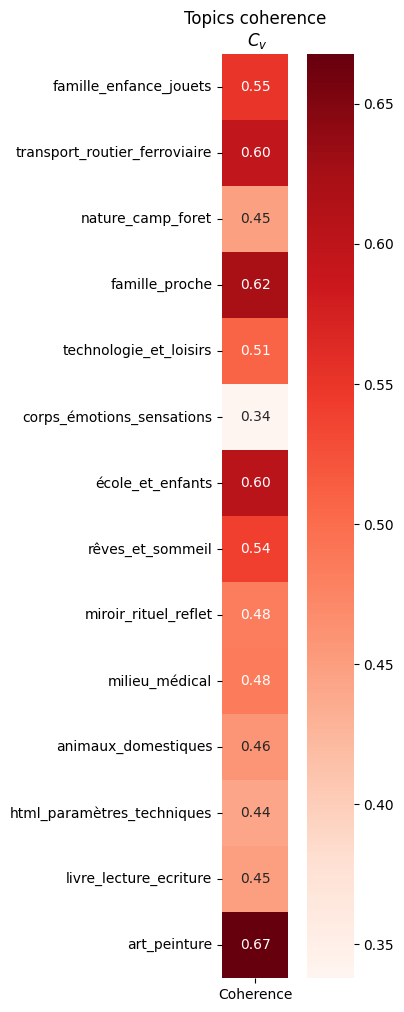
\includegraphics[width=0.5\linewidth]{illustration/coherence_corpus.png}
    \caption{Mesure de la cohérence des sujets appliquée au corpus de creepypastas}
    \label{fig:coherence_corpus}
\end{subfigure}
\centering
\begin{subfigure}[b]{0.45\textwidth}
    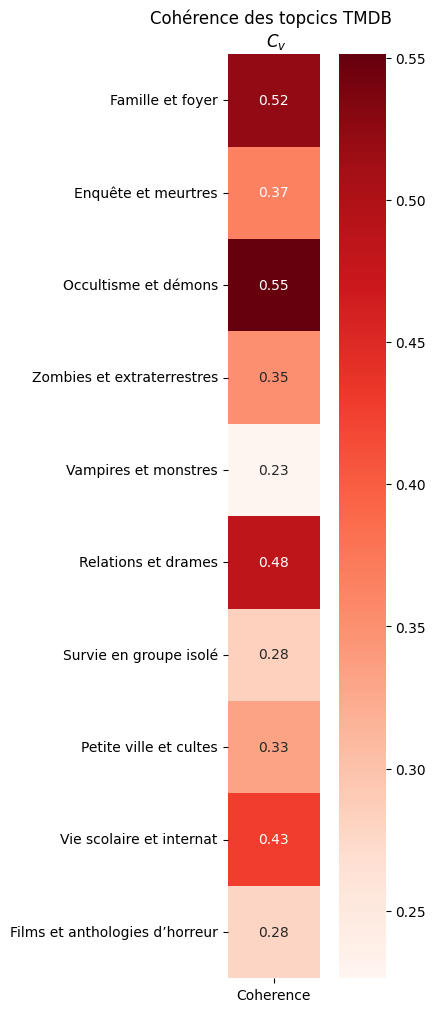
\includegraphics[width=0.5\linewidth]{illustration/coherence_tmdb.png}
    \caption{Mesure de la cohérence des sujets issus de TMDB appliquée au corpus de creepypastas}
    \label{fig:coherence_tmdb}
\end{subfigure}
\end{figure}

Dans un premier temps, nous pouvons confirmer l'hypothèse de thème spécifique à chaque genre : les mesures des cohérences systématiquement plus basses pour les topics spectaculaires comme les vampires et les aliens. En plus d'une moyenne plus basse (0,37 vs 0,48), les scores trop bas d'un côté et les scores plus élevés en lien avec l'intimité (\texttt{vie scolaire, relations, famille}) de l'autre sont autant d'éléments qui nous confortent dans ce sens. 

On note néanmoins que les mesures de cohérence des sujets issus du corpus principal présentent des résultats plus contrastés. Si certaines valeurs atteignent effectivement les niveaux élevés attendus – comme c'est le cas pour le thème \texttt{famille et école} –, la valeur obtenue pour le sujet \texttt{corps} s'avère particulièrement surprenante au regard de sa faible cohérence interne. Cette observation devient d'autant plus intrigante que ce thème apparaît, après attribution des sujets aux textes, dans plus de 5700 documents du corpus, témoignant d'une présence quantitativement significative.
Cette apparente contradiction s'explique par la nature composite de ce sujet thématique. Le thème \texttt{corps} agrège en réalité plusieurs micro-thèmes distincts (corps physique, émotions, perception, action) dont les mots-clés, bien qu'apparaissant individuellement avec une fréquence élevée dans le corpus, ne se manifestent pas nécessairement dans des contextes sémantiques similaires. Cette dispersion contextuelle explique simultanément la présence étendue de ce sujet dans le corpus et sa cohérence thématique relativement faible : les termes associés au "corps" couvrent un spectre sémantique suffisamment large pour être mobilisés dans des contextes discursifs variés, sans pour autant constituer un ensemble thématique homogène au sens strict.



\subsection{Émotions : détection et comparaison de méthodes}


Pour conclure cette tentative de caractérisation du genre, nous avons entrepris un processus de détection d'émotions automatique. Dans le cadre de l'étude d'une littérature horrifique, notre but est dans un premier temps de mettre en évidence la présence accrue de la peur. Mais comme nous l'avons affirmé précédemment, la peur dans le cadre des CP est plus insidieuse, subtile, et peut être en partie éclipsée par d'autres émotions. 

La première méthode, la plus simple aussi bien en termes de computation que de conception, avec laquelle nous avons expérimenté, utilise un système de dictionnaire annoté manuellement, le \emph{NRC Word-Emotion Association Lexcion}\footcite{mohammad_crowdsourcing_2013}, où chaque mot est associé à une émotion. Le calcul d'attribution d'une émotion à un texte consiste en la somme des occurrences de mots associés à une émotion.  %à revoir

Les premiers résultats obtenus(\ref{fig:emotions_nrc}) confirment que l'approche par vocabulaire ne révèle pas uniquement de la peur mais d'autres émotions en quantité quasi-équivalente. C'est le cas notamment de la confiance, de l'anticipation et de la tristesse. 
Les valeurs hautes au sein du corpus de ces émotions vont dans le sens d'une littérature horrifique qui ne se dit pas:  la peur apparaît peu à travers le vocabulaire. L'anticipation et la confiance sont particulièrement intéressantes: le déploiement de ces champs lexicaux implique que le narrateur ou le protagoniste est en proie à ces sentiments. L'hypothèse d'identité lecteur / personnage, que nous avons identifiée précédemment, implique que le lecteur lui aussi construit de l'attente et de la confiance : autant d'éléments qui rendent la chute finale plus déstabilisante. 
Notons aussi la quasi-absence de surprise : les textes ne semblent pas jouer avec des retournements de situation qui prendraient de court le personnage, mais construisent de l'attente à travers la confiance. 




\begin{figure}
    \centering
    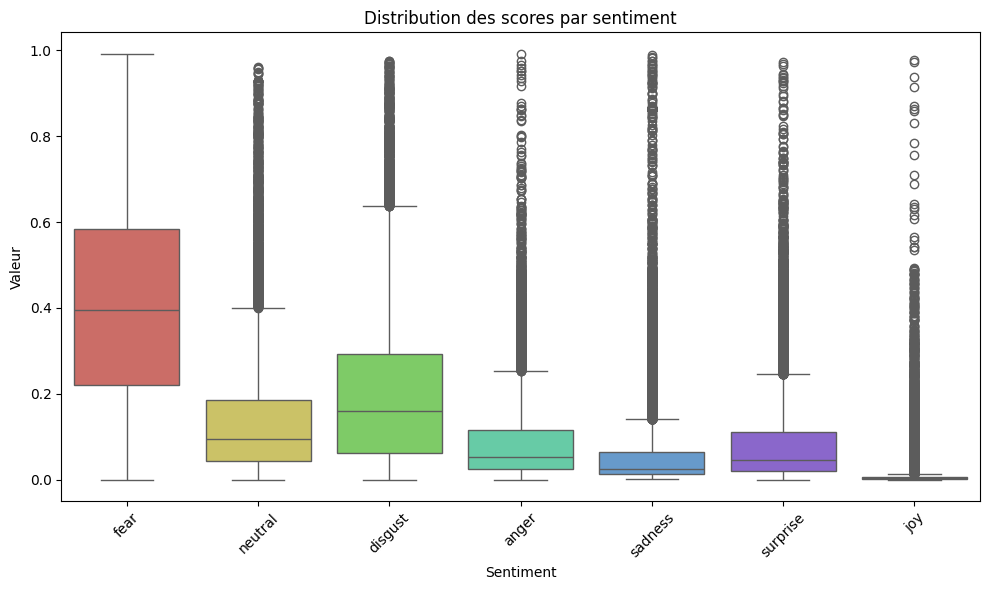
\includegraphics[width=0.5\linewidth]{illustration/emotions_bert.png}
    \caption{Distribution des scores d'émotions obtenus grâce à un modèle BERT}
    \label{fig:bert_emotion}
\end{figure}



\begin{figure}
    \centering
    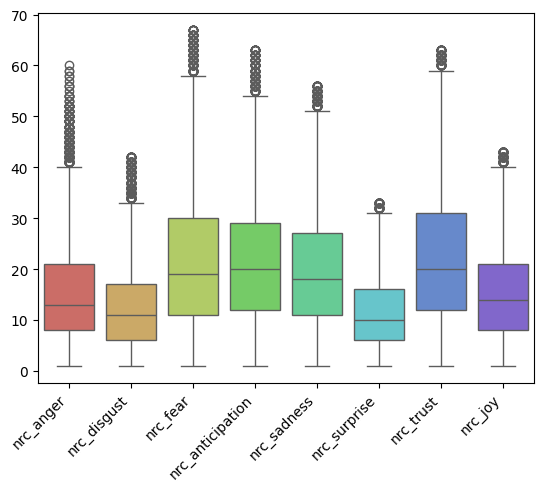
\includegraphics[width=0.5\linewidth]{illustration/nrc_emotionspng.png}
    \caption{Distribution des scores d'émotions obtenus avec le NRCLex}
    \label{fig:emotions_nrc}
\end{figure}


La seconde méthode que nous avons employée repose sur l'utilisation d'un modèle transformer BERT\footcite{hartmann2022emotionenglish} entraîné pour la détection d'émotions sur texte anglophone.

La particularité de ces modèles repose sur l'architecture \texttt{Transformers} : contrairement à une approche purement syntaxique ou lexicale, les transformers sont dotés d'un module d'attention \footcite{attention2017}, un mécanisme permettant aux modèles de constamment prendre en compte le contexte, d'avoir une \og mémoire \fg{}. Cette prise en compte du contexte est cruciale, particulièrement après les conclusions de l'approche par dictionnaire, elle permet de détecter des émotions qui dépendent du sémantisme des mots en fonction des mots adjacents et non d'une interprétation figée pour chacun d'eux. La matrice de corrélation (\ref{fig:corr_emotions}) entre les résultats issus des deux méthodes le montre bien,les différentes métriques, même lorsqu'elles mesurent la même émotion, ne sont pas ou peu corrélées : ainsi, les deux méthodes permettent d'obtenir des conclusions différentes mais complémentaires.


Les résultats de l'analyse émotionnelle automatisée (Figure \ref{fig:bert_emotion}) confirment de manière probante la centralité de la peur dans le corpus des creepypastas. Cette prédominance se manifeste à travers plusieurs indicateurs convergents : non seulement la médiane des scores de peur dépasse systématiquement le troisième quartile (Q3) de l'ensemble des autres émotions analysées, mais la dispersion des valeurs témoigne également d'une constance remarquable de cette émotion à travers le corpus. Ce résultat vient corroborer empiriquement l'intuition générique selon laquelle la peur constitue l'affect central du genre horrifique numérique.

Toutefois, l'interprétation de ces données nécessite une mise en perspective méthodologique importante. Le modèle BERT employé génère des scores de probabilité normalisés pour chaque segment textuel, ces valeurs représentent des fréquences relatives dont la somme équivaut à 1. Cette contrainte mathématique implique qu'un score élevé pour la peur (par exemple 0,7) induit mécaniquement une répartition résiduelle des autres émotions sur les 0,3 restants. Ainsi, la dominance observée de la peur reflète certes une spécificité générique réelle, mais elle est également amplifiée par la structure même de la mesure. Ainsi, il est nécessaire d'interpréter les écarts observés comme des tendances relatives plutôt que comme des valeurs absolues, tout en confirmant néanmoins la fonction structurante de la peur dans l'économie émotionnelle des creepypastas.


\begin{figure}
    \centering
    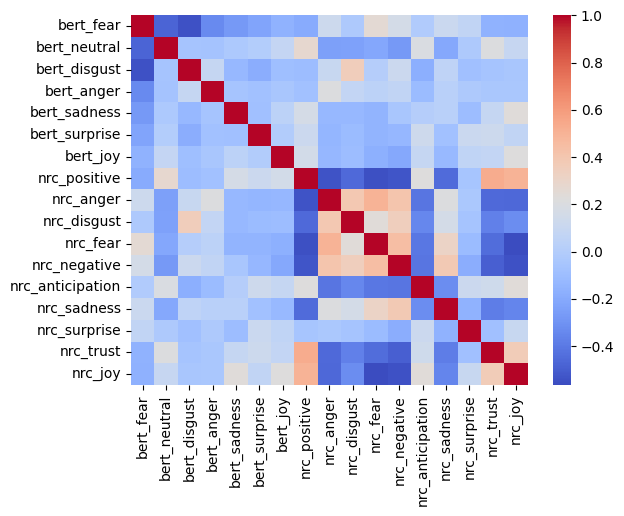
\includegraphics[width=0.5\linewidth]{illustration/nrc_bert_corr.png}
    \caption{Carte de chaleur de la corrélation des indices obtenus}
    \label{fig:corr_emotions}
\end{figure}


\section{Conclusion}

Ce panorama d'outil et de métriques obtenues par méthodes computationnelles nous permet de mieux saisir certains éléments de caractérisation des CP. 
\par
D'un point de vue syntaxique et formel tout d'abord,  les CP brillent par leur simplicité. Les productions sont très courtes et accessibles. Les phrases courtes et le vocabulaire simple rendent les textes lisibles par le plus grand nombre, ce qui est en accord avec un des éléments de définition des CP : le rapport à la viralité. Celle-ci semble prendre le pas sur la littérarité d'un point de vue syntaxique, il vaut mieux faire simple que complexe.

\par Concernant les thèmes, nous avons pu observer une différence majeure avec les stéréotypes du genre : les thèmes mobilisés sont ceux de l'expérience, de l'intime et des relations, floutant la limite entre le cadre et l'élément déclencheur de l'horreur.

\par Ces différentes observations nous permettent d'avancer l'idée d'une certaine subtilité dans les productions : le but n'est pas tant de faire sursauter, d'en appeler au gore, mais bien de questionner, de déstabiliser, en mettant en scène le quotidien et l'expérience personnelle, facilitant ainsi l'immersion du lecteur dans le texte.



\chapter[La recette du succès]{Rendre compte des dynamiques : régressions et modélisation de transmission}

Toutes les histoires ne connaissent pas la même trajectoire : au-delà des considérations esthétiques, certaines obtiennent un succès remarquable et deviennent des références durables – ce sont les CP historiques mentionnés précédemment. 

Cette section poursuit un double objectif.

Dans un premier temps, caractériser les histoires à succès à partir des données collectées dans cette étude afin d'identifier les caractéristiques quantifiables qui distinguent les œuvres ayant connu une trajectoire exceptionnelle.

Dans un second temps, tester l'application d'un modèle évolutionniste sur un ensemble plus large d'histoires pour évaluer sa capacité à expliquer la transmission et la persistance culturelle des thèmes dans les récits. 

\section{Expliquer le succès: régression logistique}

Le but de cette partie est d'explorer les différences entre les deux corpus et de rechercher quels éléments quantitatifs pourraient expliquer le succès d'une histoire par rapport à une autre. Pour ce faire, nous avons procédé en deux temps:
\begin{itemize}
\item  Dans un premier temps, nous avons cherché à identifier parmi les variables calculées précédemment les plus pertinentes pour comprendre les différences entre les histoires. 

\item  Une fois les variables identifiées, nous avons procédé à une analyse statistique pour déterminer l'impact de ces variables sur le succès des histoires. Nous avons utilisé des techniques de régression pour modéliser les relations entre les variables indépendantes (les facteurs identifiés) et la variable dépendante (le succès de l'histoire). 
\end{itemize}

\subsection{Identification des variables pertinentes : la régression pas à pas }

Afin de réaliser une régression de bonne qualité, il convient de sélectionner des variables à la fois pertinentes et dé-corrélées. En effet, la corrélation des variables peut entraîner des problèmes de multicolinéarité, rendant les coefficients de la régression instables et difficiles à interpréter. Pour ce faire, il est nécessaire de réduire le nombre de variables pour ne garder qu'un nombre plus restreint mais plus explicatif. 

Dans un premier temps, nous avons envisagé d'agréger les différents indices en fonction de la catégorie mesurée (lisibilité, richesse lexicale...). Mais les différentes mesures de corrélation tendent à montrer que chaque indice montre quelque chose de différent, et donc vaut en tant que tel.


Afin de sélectionner les variables les plus pertinentes et d'éliminer une partie des problèmes de corrélations entre variables, nous avons procédé à une première régression dite séquentielle (\emph{stepwise regression}).  Le principe de cette régression est le suivant : l'algorithme part d'un modèle vide et vient ajouter progressivement les variables, tout en mesurant l'effet de la nouvelle variable. Si celle-ci est statistiquement significative, elle est conservée. Puis l'inverse, c'est-à-dire la suppression des variables sélectionnées, est réalisé pour s'assurer de la pertinence des variables sélectionnées. Les variables sont enlevées au fur et à mesure tout en suivant la même logique. 
Dans le cas présent, nous avons comparé deux critères pour sélectionner les variables explicatives, le critère d'information d'Akaike\footcite{Akaike1998} et le critère d'information Bayésien\footcite{schwarz1978estimating}.

Dans tous les essais effectués, le critère d'information Bayésien propose un choix de variables plus restreint et significativement moins bon une fois le modèle ajusté à celles-ci. La variance expliquée par le modèle est divisée par un ordre de grandeur de 4 en passant par ce critère. Ainsi, nous avons privilégié le critère d'information d'Akaike.

Une fois ces variables sélectionnées grâce à ce critère, on applique un algorithme de régression logistique sur notre corpus limité aux-dites variables. 


\subsection{Méthode de régression et optimisation}


\begin{align*}
\log\left(\frac{P(Y=1)}{1 - P(Y=1)}\right) &= \beta_0 
+ \sum_{i=1}^{n_{\text{thème}}} \beta_{\text{thème},i} X_{\text{thème},i} \\
&\quad + \sum_{j=1}^{n_{\text{émotion}}} \beta_{\text{émotion},j} X_{\text{émotion},j} \\
&\quad + \sum_{k=1}^{n_{\text{lisibilité}}} \beta_{\text{lisibilité},k} X_{\text{lisibilité},k} \\
&\quad + \beta_{\text{longueur}} X_{\text{longueur}} 
+ \beta_{\text{mots}} X_{\text{mots}}
\end{align*}

où :
\begin{itemize}
    \item \(P(Y=1)\) est la probabilité qu’un texte devienne canonique,
    \item \(\beta_0\) est l’ordonnée à l’origine,
    \item \(\beta_{\text{thème},i}\) sont les coefficients associés aux thèmes, pour \(i = 1 \dots n_{\text{thème}}\),
    \item \(\beta_{\text{émotion},j}\) sont les coefficients associés aux émotions, pour \(j = 1 \dots n_{\text{émotion}}\),
    \item \(\beta_{\text{lisibilité},k}\) sont les coefficients associés aux indices de lisibilité, pour \(k = 1 \dots n_{\text{lisibilité}}\),
    \item \(\beta_{\text{richesse\_lexicale},k}\) sont les coefficients associés aux indices de richesse lexiclaes, pour \(k = 1 \dots n_{\text{richesse\_lexicale}}\),
    \item \(\beta_{\text{longueur}}\) est le coefficient associé à la longueur moyenne des phrases (en nombre de mots),
    \item \(\beta_{\text{mots}}\) est le coefficient associé au nombre total de mots.
\end{itemize}

Afin d'explorer le poids des différentes variables sur la canonicité des histoires, nous avons fait le choix de la régression logistique, au détriment d'autre méthode statistique de classification. En effet cette tâche, dire si un texte est canonique ou non, relève de la classification et appelle, assez naturellement, à l'utilisation de modèle du même nom ('classifier') afin de mesurer à quel point les deux corpus sont distincts. Néanmoins ces approches, contrairement à la régression logistique, sont plus dures à interpréter et souffrent souvent d'une certaine opacité. Même si un classifier est bon, il n'est pas trivial de partir en quête des éléments déterminants dans la classification. 
Ainsi, en plus d'être moins gourmand en termes de temps et de computation, la régression logistique nous permet de proposer, à la sortie du modèle, des interprétations. 

Le point de comparaison principal de cette partie est constitué de la régression logistique finale de la première version de cette étude. 
Cette régression \ref{table:logit_prem_année}, réalisée avec 15 indices retenus après la régression \textit{stepwise}, nous permettait d'obtenir un modèle intéressant mais trop peu explicatif. Malgré un modèle très significatif (\texttt{LLR p-Value}= 2,7e-43), le modèle n'expliquait que 6,5\% de la variance (\texttt{$\text{Pseudo-R}^2$ } = 0,065).

L'objectif de cette seconde version est de voir si l'amélioration du corpus canonique et l'ajout de variables, permettent d'améliorer ces résultats.


\subsection{Résultats de la régression}




\begin{table}[htbp]
\centering
\caption{Résultats de la régression logistique (variable dépendante : \texttt{is\_canon})}
\begin{tabular}{lrrrrr}
\toprule
\textbf{Variable} & \textbf{Coef.} & \textbf{Erreur std.} & \textbf{z} & \textbf{p-valeur} & \textbf{[0.025, 0.975]} \\
\midrule
intercept                        & -87.7374 & 5.938  & 14.777 & 0.000 & [76.100, 99.375] \\
passive\_verb\_ratio         & 7.1352  & 1.144  & 6.235  & 0.000 & [4.892, 9.378] \\
fear                         & -1.6684 & 0.251  & -6.640 & 0.000 & [-2.161, -1.176] \\
SMOG Index                   & 0.5331  & 0.083  & 6.400  & 0.000 & [0.370, 0.696] \\
Hapax Legomena               & -0.0009 & 0.000  & -2.413 & 0.016 & [-0.002, -0.000] \\
famille\_enfance\_jouets     & 0.6247  & 0.273  & 2.288  & 0.022 & [0.090, 1.160] \\
sadness                      & -1.8226 & 0.513  & -3.553 & 0.000 & [-2.828, -0.817] \\
nombre\_mots                 & 0.0007  & 0.000  & 1.435  & 0.151 & [-0.000, 0.002] \\
longueur\_texte              & -0.0001 & 0.000  & -1.369 & 0.171 & [-0.000, 0.000] \\
Gunning Fog Index            & -0.5360 & 0.139  & -3.865 & 0.000 & [-0.808, -0.264] \\
longueur\_phrase             & 1.8849  & 0.091  & 20.626 & 0.000 & [1.706, 2.064] \\
Flesch-Kincaid Grade Level   & -7.1831 & 0.423  & -16.976& 0.000 & [-8.012, -6.354] \\
Flesch Reading Ease          & -0.9979 & 0.059  & -16.899& 0.000 & [-1.114, -0.882] \\
Densité Lexicale             & 5.2189  & 1.374  & 3.798  & 0.000 & [2.525, 7.912] \\
technologie\_et\_loisirs     & 0.6587  & 0.238  & 2.771  & 0.006 & [0.193, 1.125] \\
famille\_proche              & -0.6692 & 0.283  & -2.361 & 0.018 & [-1.225, -0.114] \\
anger                        & -1.1595 & 0.609  & -1.905 & 0.057 & [-2.352, 0.033] \\
joy                          & -2.3641 & 1.461  & -1.618 & 0.106 & [-5.228, 0.500] \\
miroir\_rituel\_reflet       & 0.5138  & 0.292  & 1.757  & 0.079 & [-0.059, 1.087] \\
\midrule
\textbf{Log-Likelihood}      & \multicolumn{4}{c}{-1470.3} \\
\textbf{Pseudo R-squared}    & \multicolumn{4}{c}{0.2268} \\
\textbf{LLR p-value}         & \multicolumn{4}{c}{$1.492 \times 10^{-171}$} \\
\bottomrule
\end{tabular}
\label{table:logit_année_2}
\end{table}

\subsubsection{Les scores globaux}

Comme évoqué précédemment , a qualité d'une régression se mesure dans un premier temps avec la valeur $\texttt{Pseudo-R}^2$ . On note une amélioration significative de la variance expliquée avec cette version : celle-ci est multipliée quasiment par 3. 
Cela nous permet d'atteindre le seuil critique des 20\% , valeur à partir de laquelle on peut considérer qu'une régression logistique est pertinente. 

En plus du $\texttt{Pseudo-R}^2$, la \texttt{LLR p-value} est quasiment égale à 0\footnote{$0,\underbrace{000\ldots000}_{170\ \text{zeros}}1492$
}, en dessous du seuil admis de 0.05 à partir duquel on considère qu'un modèle est significatif.

\subsubsection{Les variables explicatives}

Avant de rentrer dans le détail des coefficients, on peut noter deux éléments cruciaux.
Dans un premier temps les \texttt{p-values} des variables sont majoritairement sous le seuil critique de 0.05, démontrant la pertinence des variables dans le cadre de ce modèle. Ainsi nous conserverons ces variables dans le détail de notre analyse. 
Dans un second temps, il convient d'analyser la valeur assez extrême de l'\textit{intercept}. Cette indice mesure la situation nulle, autrement dit le cas où aucune variable est prise en compte. Sans surprise, cette mesure indique une probabilité quasi nulle d'être canon "au hasard". Rappelons que les histoires canoniques ne sont qu'une infime minorité (moins d'1\%) dans l'océan que représente les CP.

Afin de visualiser au mieux le poids que représentent les variables en fonction de leur coefficient, nous avons opté pour la visualisation des rapports de côte (odd ratio). Les valeurs des coefficients données par la régression sont fonction du logarithme et ne représentent pas directement le poids que l'augmentation d'une unité peut avoir sur la probabilité d'être canon. 
Ainsi l'exponentiation des résultats permet de mieux rendre compte de l'effet.

La représentation des effets de variables(\ref{fig:logit_odd_ratios}) nous offre une conclusion intéressante.

La domination écrasante des variables stylistiques constitue la première conclusion de cette analyse. L'usage de la voix passive, avec un odds ratio dépassant 1000, se révèle être le facteur le plus discriminant de notre modèle.

Le paradoxe de la lisibilité émerge comme un résultat contre-intuitif majeur. Les indices traditionnels d'accessibilité textuelle - Flesch-Kincaid et Flesch Reading Ease - présentent des effets négatifs sur la canonisation. 

Les variables thématiques révèlent un rôle de modulation plutôt que de détermination, avec des odds ratios situés autour de 2. Les thématiques liées à la famille/enfance et à la technologie/loisirs exercent des influences positives mesurables mais limitées. 

L'analyse des dimensions émotionnelles révèle une logique de la subtilité. Les émotions négatives directement exprimées - peur, tristesse - présentent des effets inhibiteurs, suggérant que les histoires canoniques ne puisent pas leur force dans l'expression frontale d'affects négatifs.



\begin{figure}
    \centering
    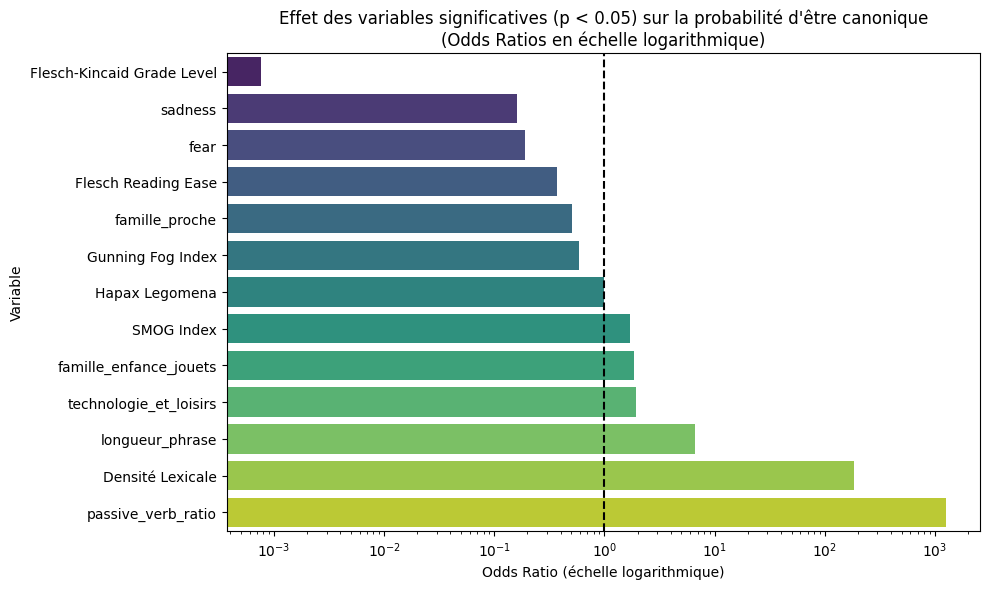
\includegraphics[width=\linewidth]{illustration/odd_ratios_logit.png}
    \caption{Visualisation des variables explicatives}
    \label{fig:logit_odd_ratios}
\end{figure}


\subsection{Conclusion de la régression}

Les expérimentations successives menées sur le corpus semblent avoir permis d'améliorer notre modèle de régression et d'accéder à des conclusions à la fois intéressantes et révélatrices. Les histoires canoniques, qui ont connu un plus grand succès sur, et en dehors des plateformes, paraissent présenter une complexité plus marquée, ce qui tend à nuancer l'hypothèse d'une littérature spécifiquement virale et donc nécessairement facile d'accès.

Dans un premier temps, le poids de la voix passive dans les productions canoniques suggère que le style de ces histoires tend vers un registre plus littéraire, potentiellement moins immédiatement accessible. Cette observation se trouve renforcée par le poids négatif des indices de lisibilité, et particulièrement du Flesch-Kincaid Grade Level. Les histoires canoniques apparaissent comme significativement plus difficiles d'accès dans cette configuration méthodologique.

Les poids sensiblement plus faibles des indices affectifs ou thématiques semblent indiquer qu'ils fonctionnent davantage comme des variables d'ajustement, suggérant ainsi une importance potentiellement plus grande de la forme par rapport aux thèmes ou au contenu. Les sentiments ne paraissent pas jouer un rôle prédominant dans cette dynamique, ce qui pourrait impliquer l'existence d'une littérature de l'implicite, où la dimension émotionnelle s'exprime de manière plus subtile ou indirecte.



\section{Expliquer les trajectoires:  Description et tentative de modélisation}
%Amorce
La tentative de régression nous a fourni des premières pistes solides quant à l'explication du caractère historique de certaines histoires. Ces conclusions semblent indiquer l'importance de la forme des récits, avec une place moindre laissée au fond.

Pour autant, ces conclusions, comme nous l'avons vu, sont difficiles à généraliser, tant la part d'histoires canoniques reste minime. Ces histoires semblent porter un caractère exceptionnel notable malgré les ressemblances naturelles avec le reste du corpus. Si ces histoires sont structurantes dans l'imaginaire lié au creepypasta, il demeure difficile de conclure, à ce stade, qu'elles constituent des éléments de référence formelle.

À l'inverse des structures syntaxiques ou lexicales, les thèmes les plus fréquents sont présents à travers tout le corpus. Cette stabilité nous servira de point de départ pour la modélisation.
Nous avons développé précédemment la théorie du mème et montré que les creepypastas s'y incluent pleinement. Au sein de ce développement, nous avons émis l'hypothèse que la transmission au sein des creepypastas repose sur des unités plus simples qu'une forme narrative générale (voir \ref{meme_fidelité}). Alors, la piste que nous allons explorer est celle des thèmes.

Un thème fonctionne comme une unité discrète facilement transmissible et peut être aisément identifiée, extraite puis réinjectée dans d'autres histoires, indépendamment de la forme qu'elle prend. Cette modularité thématique permet de pallier le problème de l'absence de filiation évidente,  il n'y a pas, en théorie comme en pratique, de moyen de déterminer avec certitude si une histoire a généré une autre histoire.

L'objectif de cette étude est de vérifier deux hypothèses, premièrement que le genre s'est structuré naturellement autour de thèmes de façon émergente ; deuxièmement que la pression sélective communautaire que nous avons pu observer se reflète dans le modèle.

Afin d'explorer ces dynamiques de reproductions successives, copie après copie, nous avons utilisé une variation du modèle de Wright-Fisher adaptée à notre corpus culturel. Avant cela, prenons le temps d'analyser nos données.

\subsection{Exploration des données}

Nous avons choisi pour cette première tentative de modélisation le corpus tiré de la plateforme creepypasta.fandom.com. Ce choix répond à une contrainte méthodologique précise, la présence d'un système de catégorisation thématique homogène et validé par une équipe de modération.

Cette infrastructure présente un double avantage. Elle garantit a priori d'abord la cohérence du balisage thématique, évitant les inconsistances terminologiques des systèmes de classification libres. Elle assure ensuite la qualité du corpus en appliquant des critères constants d'attribution des catégories.

Le site propose au moment de la récupération des données, 169 catégories. Ce nombre relativement élevé au vu du corpus composé de 13000 histoires doit être relativisé.
En effet, certaines catégories occupent une place beaucoup plus importante que les autres : 
La répartition (voir \ref{fig:rep_cat}) montre que certaines classes occupent près de 25\% du corpus à elle seule. 
Il est important de noter que chaque histoire peut être associée à plusieurs thèmes. Ainsi nous avons fait en sorte d'obtenir pour les premières représentations une répartition du nombre d’occurrences par classe. Une fois cumulée, on obtient un nombre d'occurrences plus élevé que le nombre de documents total. 
Par exemple la première classe en nombre d'occurrences compte 3158 documents, sur 30909 occurrences de thème au total, soit presque 10\%. Ainsi nous prendrons le temps de rappeler lorsque nécessaire cette distinction.

\begin{figure}
    \centering
    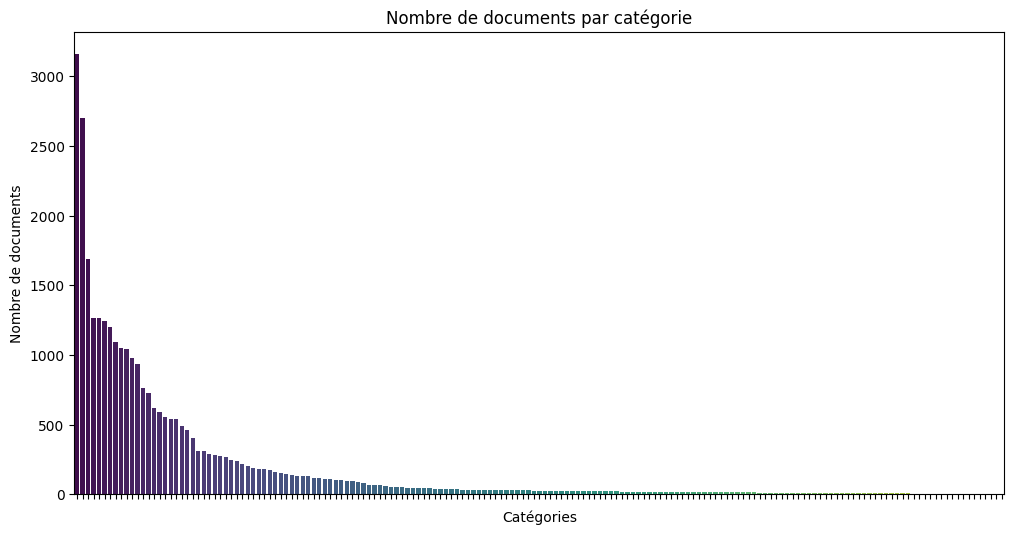
\includegraphics[width=0.5\linewidth]{illustration/rep_categories.png}
    \caption{Distribution des catégories en fonction du nombre de document associé}
    \label{fig:rep_cat}
\end{figure}

Cette prédominance de grands thèmes face aux autres plus petits se confirme d'autant plus en passant à une échelle logarithmique \ref{fig:log_log} : 

\begin{figure}
    \centering
    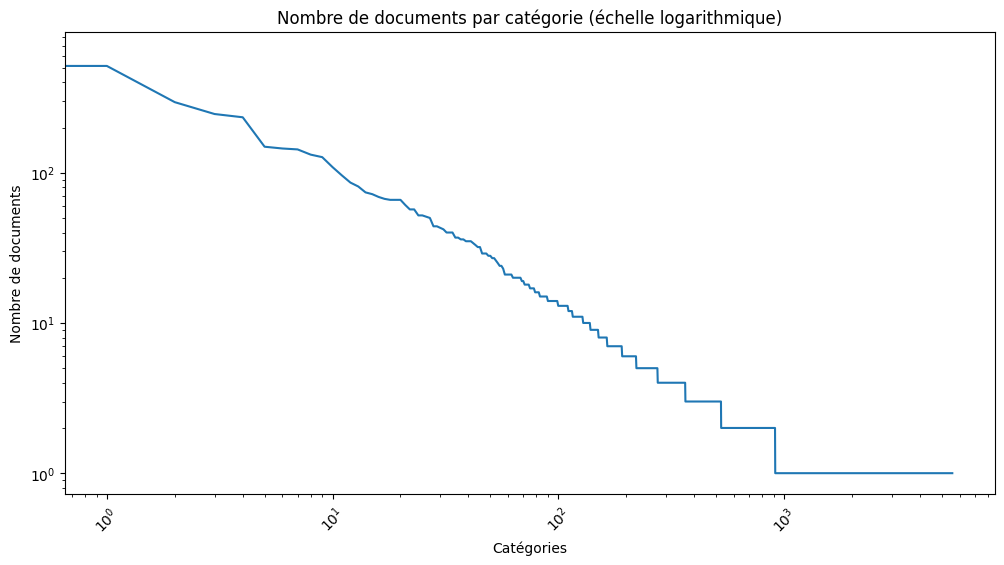
\includegraphics[width=0.5\linewidth]{illustration/log_log_cat.png}
    \caption{Nombre de document par catégorie (échelle logarithmique)}
    \label{fig:log_log}
\end{figure}
La grande majorité des classes sont quasiment vides, et un groupe de quelques classes est dominant: on voit se dessiner clairement une progression en loi de puissance. 

Cet état du corpus correspond à un moment fixe dans le temps, le moment de la récupération. Il convient maintenant de regarder la progression dans le temps de ces mêmes données afin de préparer notre modélisation. 

\begin{figure}
    \centering
    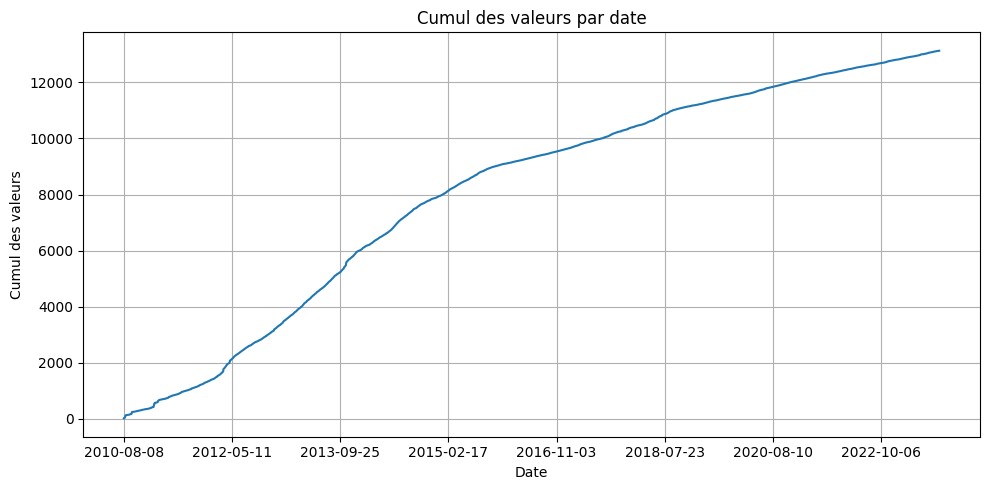
\includegraphics[width=0.5\linewidth]{illustration/evol_gen.png}
    \caption{Évolution dans le temps du nombre de productions}
    \label{fig:prod_temps}
\end{figure}
Dans un premier temps, on peut noter que le site accueille continuellement depuis 2010, sa création,  de nouvelles productions. Néanmoins le rythme de production n'a pas été constant, on remarque assez vite une rupture aux alentours de 2015, où le rythme de parution semble décroître. 

Ce point pivot est confirmé lorsqu'on regarde l'évolution des fréquences relatives de chaque catégorie (\ref{fig:freq_relative_cat}): 
\begin{figure}
    \centering
    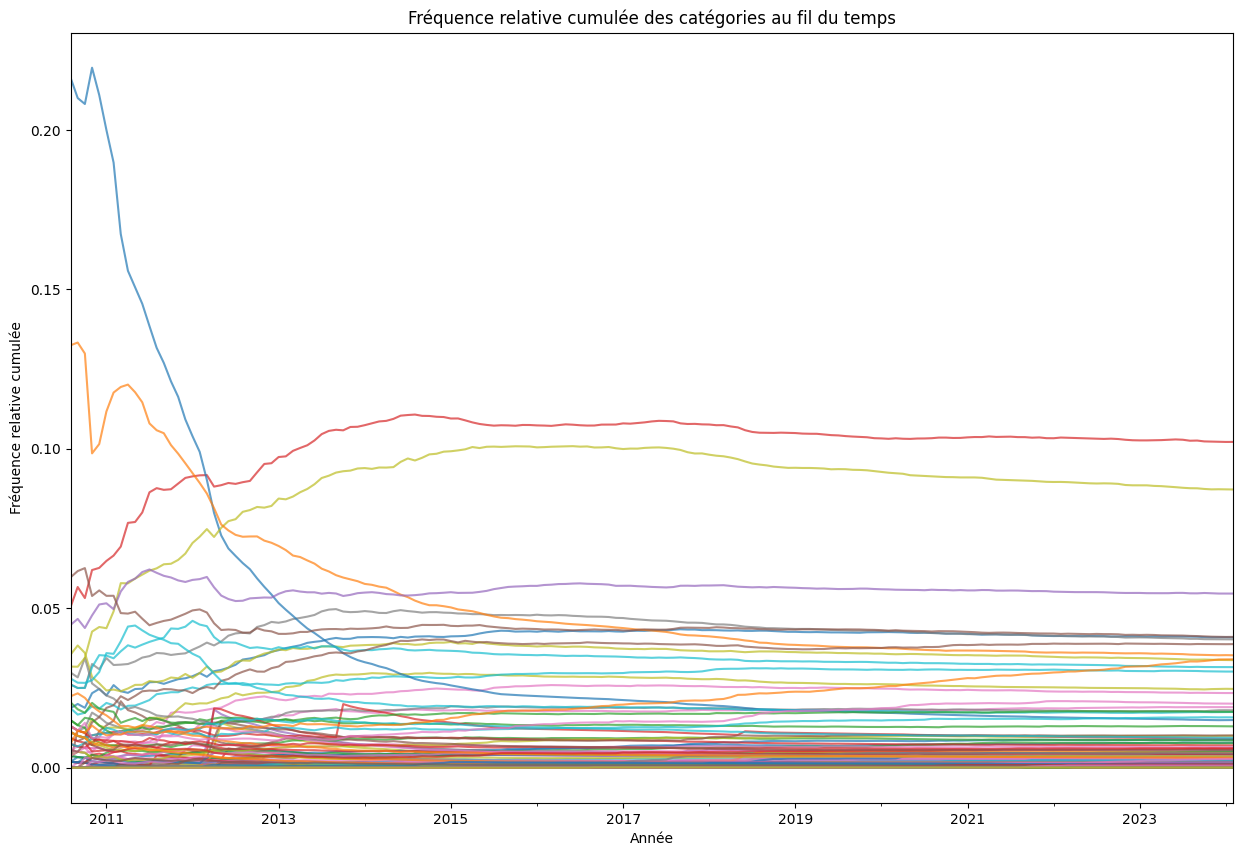
\includegraphics[width=0.5\linewidth]{illustration/freq_cat_temps.png}
    \caption{Évolution des fréquences relatives des catégories}
    \label{fig:freq_relative_cat}
\end{figure}

Dans un premier temps, on remarque que les proportions relatives de chaque catégorie se stabilisent vite dans le temps. Et particulièrement à partir des alentours des années 2015. 

Ce figement est intriguant : le fait qu'à partir de 2015, les données semblent suivre un schéma similaire, malgré l'ajout constant du nombre de production, semble indiquer que l'évolution s'est arrêtée à un état stable, impliquant donc que le site actuellement est une sorte d'instantané de l'état précédent. 
\begin{figure}
    \centering
    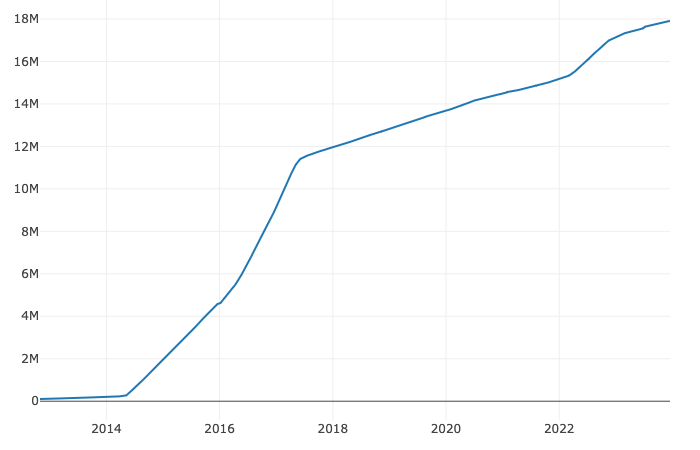
\includegraphics[width=0.5\linewidth]{illustration/subscriber_reddit.png}
    \caption{Évolution du nombre d'abonnées du subreddit /r/nosleep}
    \label{fig:sub_reddit}
\end{figure}

On peut émettre deux hypothèses quant à cette évolution. 
D'abord, l'émergence et la popularité croissante de plateformes comme Reddit, et notamment son subreddit r/nosleep, ont pu impacter les sites plus petits. On observe une baisse significative de la popularité (mesurée par le nombre de commentaires) des pages sur le fandom à partir de 2015, comme en témoigne le classement par années des pages populaires sur cette même plateforme \footnote{\url{https://creepypasta.fandom.com/wiki/Creepypasta_Wiki:Popular_Pages}}. Cette coïncidence temporelle suggère un transfert d'audience vers de nouveaux espaces de contenu.

Une autre hypothèse similaire tiendrait dans la modification des habitudes de consommation des utilisateurs en ligne. Le milieu puis la fin des années 2010 correspondent à l'avènement du smartphone comme moyen privilégié d'accès aux contenus en ligne, et donc le passage par des applications dédiées au profit de la navigation sur internet. Néanmoins, en l'absence de chiffres précis pour appuyer ce propos, nous resterons prudents quant à cette interprétation.

%Conclusion
Ainsi, l'analyse descriptive de ce corpus met en lumière deux dynamiques, déjà une croissance puis une stabilisation aussi bien concernant les thèmes que le volume de production. Nous posons ainsi l'hypothèse que notre corpus de données représente non pas une simple \og photographie instantanée\fg{} de la production active à un moment donné, mais bien un historique cumulatif de toute la production depuis son origine.

Cette rupture vers un état stable nous invite à sélectionner uniquement les données jusqu'en 2015 (inclus) pour notre modélisation, période de transformation et donc d'évolution sur la plateforme, afin de voir si la modélisation permet de confirmer cette hypothèse.

\subsection{Application et résultats du modèle de Wright-Fisher}

Afin de modéliser cette évolution, nous allons, comme convenu, utiliser le modèle Wright-Fisher.

Ce modèle\footcite{wright1931evolution} \footcite{fisher1999genetical}, développé initialement pour étudier l'évolution génétique dans des populations finies, offre un cadre intéressant pour notre analyse de la transmission au sein de la plateforme. Ce modèle probabiliste permet de simuler comment des caractères discrets évoluent au fil des générations sous l'effet combiné de la dérive aléatoire et de la sélection.

Dans sa forme classique et la plus simple, le modèle considère une population de taille fixe N où chaque individu peut porter un de deux allèles qui peuvent être transmis à la génération suivante. À chaque génération, les nouveaux individus sont formés par échantillonnage aléatoire avec remise dans la population parentale.

Dans notre cas, la "population" correspond à l'ensemble des histoires actives dans la circulation communautaire à un moment donné. Les "allèles" sont représentés par les thèmes identifiés dans notre analyse précédente. Chaque histoire pouvant porter plusieurs thèmes,

Le modèle permet de simuler un phénomène fondamental, la dérive neutre, par laquelle la fréquence des thèmes fluctue aléatoirement d'une génération à l'autre.

Si le modèle permet de pallier à l'absence de filiation directe (contrairement à d'autres modèles de spéciations) les hypothèses fortes de celui-ci sont restrictives. La présence dans sa version la plus simple de 2 allèles et d'une génération finie, par exemple, ne permet pas de rendre compte de notre cas. 

Ainsi nous avons construit un modèle Wright-Fisher avec : 
\begin{itemize}
    \item  $n$ allèles de départ 
    \item Une population qui évolue de façon linéaire
\end{itemize}


%La génération de départ

Afin de fixer la population de départ et les n catégories, nous avons exploré deux possibilités : partir d'une répartition aléatoire du nombre de classes fixe entre les différents témoins, ou bien reprendre la répartition réelle en loi de puissance afin de s'approcher de la situation de départ.

Ensuite un nombre T de générations est lancé, et nous analysons un ensemble entre 0 et t générations. 
Cette valeur t est volontairement plus basse que la valeur T : en effet, le modèle Wrigth-Fisher va, par définition, tendre vers un état de monoculture où un seul allèle va prendre le dessus et finir par saturer la population.

Ces premières tentatives sont encourageantes, mais restent peu concluantes. 

Les paramètres retenus sont les suivants : 
\begin{itemize}
    \item n = 40
    \item population de départ  = 1000
    \item population d'arrivée = 2000
    \item T = 1000
    \item t = 300
\end{itemize}

Ces simulations en l'état convergent très vite vers un état où seule une poignée de catégories subsistent sans qu'on puisse distinguer une forme de stabilité caractéristique de notre corpus (\ref{fig:wf_vanilla}).

\begin{figure}
    \centering
    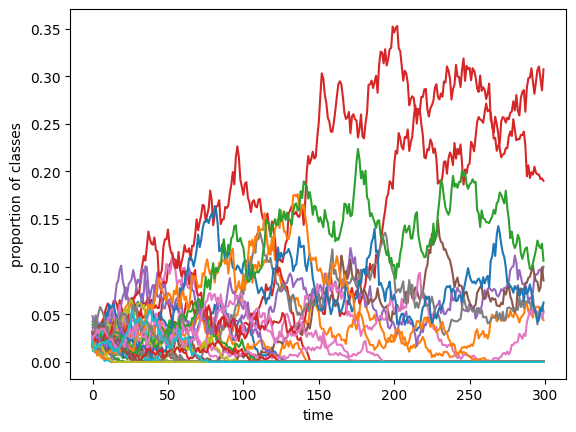
\includegraphics[width=0.5\linewidth]{illustration/wf_vanilla.png}
    \caption{Simulation Wright-Fisher avec distribution aléatoire des allèle de départ}
    \label{fig:wf_vanilla}
\end{figure}
\begin{figure}
    \centering
    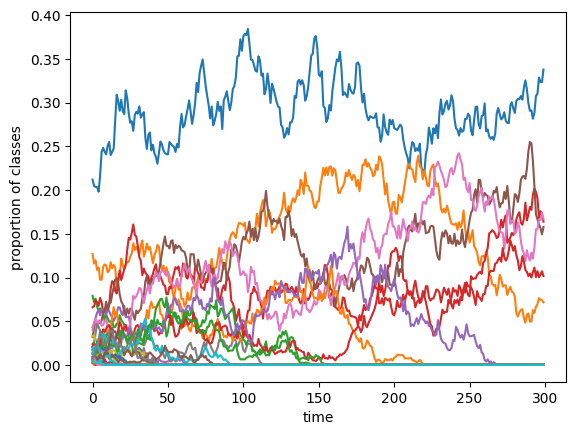
\includegraphics[width=0.5\linewidth]{illustration/wf_pow.png}
    \caption{Simulation Wright-Fisher avec distribution des allèles suivant une loi normale}
    \label{fig:wf_power}
\end{figure}

Si l'initialisation en loi de puissance a permis de conserver la dominance des classes initialement majoritaires, à l'image du phénomène de \textit{rich get richer} attendu, elle a paradoxalement accéléré l'extinction des classes minoritaires par rapport au modèle avec initialisation aléatoire, ne rendant pas compte de la longue traîne stable observée dans notre corpus réel (voir \ref{freq_relative_cat}). En effet, le graphique de fréquences cumulées des catégories réelles révèle non seulement des dominances claires, mais aussi la persistance de nombreuses catégories à de faibles proportions, sans extinction rapide.

Pour prendre en compte cet aspect cumulatif, nous avons modifié notre approche en adaptant le modèle de Wright-Fisher. Désormais, à chaque génération, un échantillon est prélevé puis archivé. C'est cette archive cumulative que nous analyserons. Le but de cette archive est de modéliser le fait que le site, à défaut de se renouveler, conserve un comportement donné au fil du temps, intégrant ainsi une "mémoire" du passé.


\begin{figure}
    \centering
    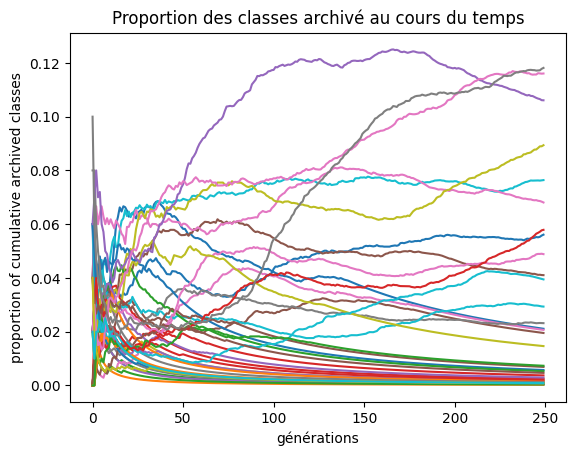
\includegraphics[width=0.5\linewidth]{illustration/wf_archive`.png}
    \caption{Simulation Wright-Fisher sur les échantillons archivés}
    \label{fig:wf_archive}
\end{figure}

Cette simulation (\ref{fig:wf_archive})(qui conserve les mêmes paramètres, à l'exception du t, que les simulations précédentes) montre une répartition beaucoup plus proche de nos observations. Après une période de fluctuation, une partie des catégories moins représentées se stabilise sans disparaître, alors que des classes majoritaires commencent à se stabiliser. L'intuition de l'ajout du cumul pour éviter l'extinction des classes les moins dotées semble confirmer l'hypothèse d'un historique cumulatif sur le site. 

Cette répartition finale, à l'instar de nos données, suit une loi de puissance (\ref{fig:loglog_archive}), avec une majorité de classes à un représentant, confirmant l'hypothèse au-delà du graphique similaire.
\begin{figure}
    \centering
    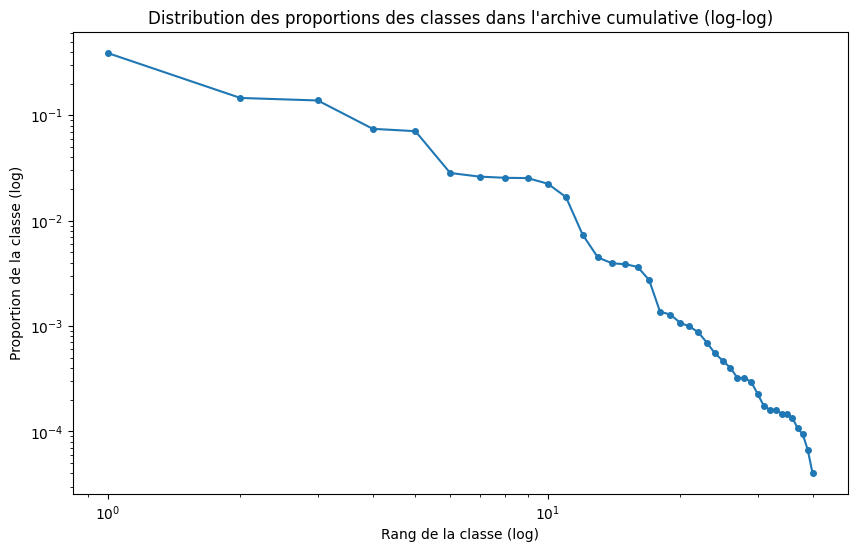
\includegraphics[width=0.5\linewidth]{illustration/loglog_archive.png}
    \caption{Distribution de la fréquence finale des allèle, échelle log log}
    \label{fig:loglog_archive}
\end{figure}


Nos simulations initiales avec le modèle de Wright-Fisher n'ont pas su reproduire la longue traîne stable de nos données réelles, les catégories minoritaires s'éteignant trop vite. Ce constat a mis en lumière l'absence de "mémoire" dans le modèle classique, pourtant essentielle pour comprendre un corpus cumulatif comme le nôtre.

L'intégration d'un mécanisme d'archivage cumulatif a transformé notre approche. En prélevant et en accumulant des échantillons à chaque génération, notre modèle a enfin pu simuler la persistance observée. La Figure \ref{fig:wf_archive} le montre clairement : les catégories minoritaires se stabilisent au lieu de disparaître, tandis que les majoritaires trouvent aussi leur équilibre.

Mieux encore, l'analyse en échelle log-log confirme que la distribution finale des classes suit une loi de puissance, exactement comme nos données réelles. Cela valide l'hypothèse d'un processus d'accumulation historique dominant le comportement de notre corpus.

En bref, l'ajout de l'archivage cumulatif au modèle de Wright-Fisher a permis de reproduire fidèlement les dynamiques de notre corpus, prouvant que la "mémoire" du système est fondamentale pour comprendre son évolution.

\part*{Conclusions et perspectives futures}
\addcontentsline{toc}{part}{Conclusion, et perspectives futures}
\markright{Conclusions}                     % Pour forcer l’en-tête droite (si classe report/book)

%Rappel pbm Ainsi nous nous demanderons comment l'analyse computationnelle des caractéristiques textuelles (formelles, thématiques et affectives) permet-elle de définir les spécificités des creepypastas en tant que genre de littérature numérique et d'identifier les facteurs contribuant à leur succès viral et à l'émergence d'un canon dans l'écosystème en ligne? }

Le présent mémoire avait pour objectif d'explorer la nature du genre des creepypastas comme littérature numérique virale. Notre question de recherche visait à déterminer comment une approche quantitative des textes pouvait, d'une part, révéler les spécificités de ce genre et, d'autre part, identifier les facteurs contribuant à l'émergence d'un canon. Grâce à une méthodologie combinant l'analyse littéraire traditionnelle et les outils des humanités numériques, notamment le Traitement Automatique des Langues (TAL), cette étude a permis de mettre en lumière un genre qui, tout en s'inscrivant dans des codes classiques, innove par une approche de création de contenu intrinsèquement liée au numérique et à Internet.

Les résultats de notre analyse confirment et nuancent plusieurs hypothèses initiales. Nous avons d'abord observé que les creepypastas, contrairement aux stéréotypes associés à la littérature d'horreur, se caractérisent par une simplicité de construction et une prédominance des thématiques de l'intime et de l'expérience quotidienne. Cette observation est étayée par l'analyse des valences émotionnelles de notre corpus, qui a révélé une présence moins marquée du lexique horrifique pur que ce à quoi on aurait pu s'attendre, suggérant que la peur dans les creepypastas s'ancre souvent dans le familier et le suggestif plutôt que dans le grotesque explicite.

De manière plus significative, notre tentative de régression logistique pour modéliser la viralité des creepypastas a mis en lumière la prévalence des variables liées à la lisibilité et à la longueur des phrases dans leur capacité à se propager, au détriment des thématiques ou de la peur elle-même. Ces résultats suggèrent que, dans le contexte de la littérature numérique virale, la forme et l'accessibilité du texte peuvent être des facteurs déterminants pour sa diffusion, dépassant potentiellement le contenu thématique intrinsèque. Cela indique que la "peur virale" n'est pas uniquement une question de contenu effrayant, mais aussi de la manière dont ce contenu est présenté et consommé en ligne.

Ces premières tentatives de modélisation ont également démontré la faisabilité de rendre compte des phénomènes d'évolution au sein d'une plateforme par un modèle simple et adapté. Elles ont notamment révélé que le poids des productions passées est crucial pour comprendre la répartition actuelle des données textuelles. Cela suggère que, même si le genre des creepypastas peut connaître un cycle de vie plus court, il se construit néanmoins par la réutilisation et la transformation des éléments narratifs et formels antérieurs, un processus fondamental dans l'émergence et la consolidation d'un canon.

Ces recherches constituent un premier pas humble et exploratoire dans un domaine encore en pleine émergence. Premièrement, elle enrichit la compréhension des genres émergents de la littérature numérique, en particulier les creepypastas, en proposant une analyse rigoureuse basée sur des données textuelles massives. Deuxièmement, elle démontre la valeur ajoutée des humanités numériques pour aborder des questions littéraires complexes, offrant de nouvelles perspectives sur la littérarité et la réception des textes en ligne. Nos découvertes sur la viralité, en particulier, ouvrent de nouvelles voies de réflexion sur les facteurs de propagation des récits en ligne, allant au-delà des approches purement thématiques.

Il est important de noter que cette étude présente certaines limites. Bien que la taille et la composition de notre corpus soient représentatives, elles ne couvrent pas l'intégralité de la diversité des creepypastas. L'échantillon utilisé, bien que conséquent, pâlit en comparaison du vaste volume d'histoires encore inexplorées qui pourraient enrichir de futures études. De même, si les conclusions de la régression logistique sont encourageantes, il convient de les nuancer, non pas par pessimisme, mais comme un appel à explorer d'autres améliorations et indices susceptibles de rendre compte plus finement de ce phénomène fascinant.

Ces découvertes ouvrent la voie à de nombreuses perspectives de recherche futures. Premièrement, il serait pertinent d'élargir le corpus à d'autres plateformes ou à d'autres langues afin de vérifier la généralisabilité de nos résultats.

Les premiers résultats encourageants de modélisation nous incitent, dans un second temps, à envisager une approche plus diachronique, tant des thèmes que de la forme, et à poursuivre les efforts de modélisation en appliquant des modèles plus sophistiqués et issus d'autres domaines.

Enfin, comme nous l'avons souligné, les creepypastas brillent par leur multimodalité. Cela appelle naturellement à une approche qui dépasse le seul texte pour explorer quantitativement les images, illustrations et vidéos associées, afin de déterminer si les conclusions tirées de l'analyse textuelle s'appliquent également aux éléments visuels.

En somme, l'exploration des creepypastas révèle un genre littéraire fascinant, où la peur se manifeste non seulement par des thèmes sombres, mais surtout par une ingéniosité formelle et une adaptation aux dynamiques de la viralité numérique. Cette recherche souligne que, dans l'ère du numérique, la peur est plus que jamais une question de contagion et de partage, et que la littérature, sous ses formes les plus inattendues, continue d'évoluer et d'interroger nos propres appréhensions dans un monde de plus en plus connecté.

\newpage
\listoffigures
\addcontentsline{toc}{chapter}{Table des figures}
\listoftables
\addcontentsline{toc}{chapter}{Tables des tables}

\appendix
	\part*{Annexe}
	\section*{Données et codes}
	Toutes les données (liens, textes et différents corpus) et tous les scripts et notebooks utilisés sont disponibles à l'adresse \texttt{github} suivante: 
	
	\begin{centering}
		\url{https://github.com/Rollybre/HN_memoire_creepypasta}
	\end{centering}
	\bigskip\\

	\section*{Les indices de lisibilité}
\begin{itemize}
		
\item \textbf{Indice de lisibilité de Flesch} : Cet indice mesure la facilité de lecture d’un texte. Les scores vont de 0 (très difficile) à 100 (très facile). La formule est :
\[
206{,}835 - 1{,}015 \times \left( \frac{\text{nombre total de mots}}{\text{nombre total de phrases}} \right) - 84{,}6 \times \left( \frac{\text{nombre total de syllabes}}{\text{nombre total de mots}} \right).
\]
Un score élevé indique une meilleure lisibilité ; des valeurs supérieures à 60 conviennent à un large public.

\item \textbf{Niveau scolaire Flesch-Kincaid} : Cet indice estime le niveau scolaire américain nécessaire pour comprendre un texte. La formule est :
\[
0{,}39 \times \left( \frac{\text{nombre total de mots}}{\text{nombre total de phrases}} \right) + 11{,}8 \times \left( \frac{\text{nombre total de syllabes}}{\text{nombre total de mots}} \right) - 15{,}59.
\]
Un niveau bas indique un texte plus simple.

\item \textbf{Indice Gunning Fog} : Cet indice évalue la complexité d’un texte en fonction de la longueur des phrases et de la proportion de mots complexes (définis comme ayant trois syllabes ou plus). La formule est :
\[
0{,}4 \times \left[ \left( \frac{\text{nombre total de mots}}{\text{nombre total de phrases}} \right) + 100 \times \left( \frac{\text{mots complexes}}{\text{nombre total de mots}} \right) \right].
\]
Un score inférieur à 8 indique une lecture facile, tandis qu’un score supérieur à 17 suggère une grande complexité.

\item \textbf{Indice SMOG (Simple Measure of Gobbledygook)} : Le SMOG estime le nombre d’années d’études nécessaires pour comprendre un texte, en se concentrant sur les mots polysyllabiques. La formule est :
\[
1{,}043 \times \sqrt{\text{nombre de mots polysyllabiques} \times \left( \frac{30}{\text{nombre de phrases}} \right)} + 3{,}1291.
\]
Cet indice est particulièrement utilisé dans le domaine de la santé pour assurer la clarté des communications.

\item \textbf{Indice de lisibilité automatisé (ARI)} : Cet indice évalue la lisibilité en fonction du nombre de caractères, de mots et de phrases. Sa formule est :
\[
4{,}71 \times \left( \frac{\text{caractères}}{\text{mots}} \right) + 0{,}5 \times \left( \frac{\text{mots}}{\text{phrases}} \right) - 21{,}43.
\]
Le résultat correspond à un niveau scolaire américain.

\item \textbf{Indice Coleman-Liau} : Cet indice estime la lisibilité en analysant le nombre de lettres et de phrases pour 100 mots. Il est défini comme suit :
\[
0{,}0588 \times L - 0{,}296 \times S - 15{,}8,
\]
où \( L \) est le nombre moyen de lettres pour 100 mots, et \( S \) le nombre moyen de phrases pour 100 mots.

\item \textbf{Indice de lisibilité Dale-Chall} : Cet indice évalue la lisibilité en prenant en compte la proportion de mots difficiles (non présents dans une liste prédéfinie de mots familiers) et la structure des phrases. La formule est :
\[
0{,}1579 \times \left( \text{pourcentage de mots difficiles} \right) + 0{,}0496 \times \left( \text{longueur moyenne des phrases} \right).
\]
Une correction est appliquée si la proportion de mots difficiles dépasse 5\%.

\item \textbf{Indice Lix} : Couramment utilisé pour les textes en suédois, cet indice mesure la lisibilité à partir de la longueur des mots et des phrases. La formule est :
\[
\text{Lix} = \frac{\text{nombre de mots}}{\text{nombre de phrases}} + 100 \times \frac{\text{mots longs (6 lettres ou plus)}}{\text{nombre total de mots}}.
\]
Un score inférieur à 25 indique un texte très simple, tandis qu’un score supérieur à 60 indique un texte très complexe.


\end{itemize}	


	

		\pagebreak
	\begin{table}[htbp]
		\centering
		\caption{Équivalents Scolaires (France) et Indices de Lisibilité en Anglais - Partie 1}
		\resizebox{\textwidth}{!}{%
			\begin{tabular}{cccc}
				\toprule
				\textbf{Équivalence Scolaire} & \textbf{Flesch Reading Ease} & \textbf{Flesch-Kincaid Grade Level} & \textbf{Gunning Fog Index} \\ \midrule
				CP - CE1                               & 90-100                           & 1.0-2.0                               & 6.0-7.0                           \\ 
				CE2 - CM1                              & 80-89                            & 3.0-4.0                               & 7.0-8.0                           \\ 
				CM2 - 6ème                              & 70-79                            & 5.0-6.0                               & 8.0-9.0                           \\
				5ème - 4ème                             & 60-69                            & 7.0-8.0                               & 9.0-10.0                         \\
				3ème - 2nde                             & 50-59                            & 9.0-10.0                              & 10.0-11.0                        \\ 
				1ère - Terminale                        & 30-49                            & 11.0-12.0                             & 11.0-12.0                        \\ 
				\bottomrule
			\end{tabular}%
		}
		\label{tab:readability_indices_part1}
	\end{table}
	
	\begin{table}[htbp]
		\centering
		\caption{Équivalents Scolaires (France) et Indices de Lisibilité en Anglais - Partie 2}
		\resizebox{\textwidth}{!}{%
			\begin{tabular}{cccc}
				\toprule
				\textbf{Équivalence Scolaire} & \textbf{SMOG Index} & \textbf{Automated Readability Index} & \textbf{Coleman-Liau Index} \\ 
				\midrule
				CP - CE1                               & 4.0                               & 1.0-2.0                                     & 1.3-2.8                                 \\ 
				CE2 - CM1                              & 5.0                               & 3.0-4.0                                     & 3.0-4.5                                 \\ 
				CM2 - 6ème                              & 6.0                               & 5.0-6.0                                     & 5.0-6.5                                 \\ 
				5ème - 4ème                             & 7.0                               & 7.0-8.0                                     & 7.0-8.5                                 \\ 
				3ème - 2nde                             & 8.0                               & 9.0-10.0                                    & 9.0-10.5                               \\ 
				1ère - Terminale                        & 9.0                               & 11.0-12.0                                   & 11.0-12.5                             \\ \bottomrule
			\end{tabular}%
		}
		\label{tab:readability_indices_part2}
	\end{table}
	
		
	
	



	\section*{Les indices de richesse lexicale}
	\label{annexe_richesse_lex}


\begin{itemize}
\item \textbf{Moving-Average Type-Token Ratio (MATTR)} : Le MATTR (\footcite{covington2010cutting}) est une extension du traditionnel Type-Token Ratio (TTR), qui corrige sa sensibilité à la longueur du texte en calculant la moyenne des TTR sur plusieurs segments de taille fixe. Cette mesure fournit une estimation plus stable de la diversité lexicale dans des textes de longueurs variées. La formule du MATTR est :
\[
\text{MATTR} = \frac{1}{N} \sum_{i=1}^{N} \frac{\text{Nombre de types dans le segment } i}{\text{Nombre de tokens dans le segment } i},
\]
où \(N\) est le nombre total de segments. Un MATTR plus élevé indique une plus grande diversité lexicale, et permet une comparaison plus fiable entre les textes en atténuant l’influence de la longueur totale. Nous utilisons ici des segments de 100 mots.

\item \textbf{Hapax legomena} : Les \textit{hapax legomena} désignent les mots qui n’apparaissent qu’une seule fois dans un texte. Leur proportion est souvent utilisée comme indicateur de richesse du vocabulaire. Elle se calcule ainsi :
\[
\text{Proportion d’hapax} = \frac{\text{Nombre d’hapax legomena}}{\text{Nombre total de mots}}.
\]
Cette métrique met en valeur la présence de mots rares ou uniques.

\item \textbf{Densité lexicale} : La densité lexicale quantifie la proportion de mots lexicaux (noms, verbes, adjectifs et adverbes) par rapport au nombre total de mots. Elle est définie comme suit :
\[
\text{Densité lexicale} = \frac{\text{Nombre de mots lexicaux}}{\text{Nombre total de mots}}.
\]
Une densité lexicale élevée suggère un texte plus informatif, souvent observé dans les écrits formels ou techniques.

\item \textbf{Indice R de Honoré} : L’indice R de Honoré est une mesure de la richesse lexicale qui prend en compte le nombre d’\textit{hapax legomena }et le nombre total de mots dans un texte. La formule est :
\[
R = 100 \times \frac{\log(\text{Nombre total de mots})}{1 - \frac{\text{Nombre d’hapax legomena}}{\text{Nombre total de mots}}}.
\]
Cette métrique est moins sensible à la longueur du texte que le TTR, et fournit une estimation robuste de la diversité du vocabulaire.
\end{itemize}


\section*{Régression logistique}
\begin{table}[htbp]
	\centering
	\caption{Résultats de la régression logistique à la fin de la première année}
	\begin{tabular}{lcccc}
		\toprule
		& \textbf{Coefficient} & \textbf{Std. Err.} & \textbf{z} & \textbf{P>|z|} \\
		\midrule
		const                        & -5.8195 & 0.213 & -27.356 & 0.000 \\
		readability & 5.7874  & 0.463 & 12.503  & 0.000 \\
		longueur\_phrase             & -2.5806 & 0.404 & -6.380  & 0.000 \\
		topic\_douleur\_physique                     & -0.6548 & 0.322 & -2.032  & 0.042 \\
		sadness                      & 0.5662  & 0.149 & 3.802   & 0.000 \\
		fear                         & -0.7814 & 0.184 & -4.252  & 0.000 \\
		anger                        & 0.2779  & 0.147 & 1.888   & 0.059 \\
		topic\_forêt                     & 1.0509  & 0.455 & 2.312   & 0.021 \\
		topic\_voiture                   & -0.7302 & 0.462 & -1.579  & 0.114 \\
		topic\_trauma                 & -1.2659 & 1.005 & -1.260  & 0.208 \\
		positive                     & -0.4414 & 0.185 & -2.389  & 0.017 \\
		joy                          & 0.2468  & 0.145 & 1.700   & 0.089 \\
		anticipation                 & -0.2893 & 0.166 & -1.745  & 0.081 \\
		surprise                     & 0.1851  & 0.129 & 1.436   & 0.151 \\
		topic\_animaux                     & -0.3851 & 0.285 & -1.349  & 0.177 \\
		\midrule
		\textbf{Log-Likelihood}      & \multicolumn{4}{c}{-1724.7} \\
		\textbf{Pseudo R-squared}    & \multicolumn{4}{c}{0.06516} \\
		\textbf{LLR p-value}         & \multicolumn{4}{c}{2.744e-43} \\
		\bottomrule
	\end{tabular}
	\label{table:logit_prem_année}
\end{table}





			\pagebreak
			\nocite{*}
	\printbibliography
\end{document}
